\documentclass[10pt, a4paper]{article}

% Page
\usepackage{pdflscape} % make certain pages landscape
\usepackage{geometry} % set page geometry
\usepackage[indent=2em, skip=0.8em plus 0.1 em minus 0.2 em]{parskip} % set paragraph spacing
\renewcommand{\floatpagefraction}{.8} % only floats taking up more than 80% of the page will get their own page

% Font and Text
\usepackage[utf8]{inputenc}
\usepackage{bbm} % blackboard bold fonts
\usepackage{lmodern} % bold teletype font
\usepackage{epigraph} % memorable quotes
\usepackage{csquotes} % allows quoting blocks of text
\usepackage{textcomp} % allow text settings
\usepackage{xcolor} % allows for colouring of source code blocks
\usepackage{url} % better URLs
\usepackage{indentfirst} % indent the first line after a heading
\usepackage{enumitem} % gives alphabet list headers

% Notation
\usepackage{amssymb} % allows for maths mode symbols
\usepackage{amsmath} % allows for many maths mode commands
\usepackage{amsthm} % allows for QED tombstone
\usepackage{mathtools}
\allowdisplaybreaks% allow display elements to break across pages
\usepackage{siunitx} % allows SI units to be formatted
\usepackage{braket} % support Dirac notation
\usepackage{esvect} % nicer vector arrows
\usepackage[thinc]{esdiff} % derivatives 
\usepackage{esint} % integrals
\usepackage{cancel} % allow cancellation
\usepackage{mleftright} % fix spacing issues in \left and \right
\mleftright % rename left/right -> mleft/mright

% Tables
\usepackage{tabulary} % allows for better tables
\usepackage{booktabs} % nice lines at top and bottom of tables
\usepackage{longtable} % allows tables to span pages
\usepackage{makecell} % allow nice table titles
\usepackage[export]{adjustbox} % allow tables to take up the space they need, and export additional scaling stuff for graphicx
\usepackage{diagbox} % diagonal box in table
\usepackage{multirow} % cells in tables can span rows/columns
\usepackage{tablefootnote} % use \tablefootnote for footnotes in tables

% Code
\usepackage{listings} % allows for source code blocks
\usepackage{algorithm} % typeset algorithms
\usepackage{algpseudocode} % pseudocode style algorithms
\usepackage{fancyvrb} % better verbatim stuff

% Document
\usepackage[backend=biber, style=ieee-alphabetic, natbib=true]{biblatex}
\addbibresource{../wiring.bib}
\graphicspath{{../images/}}
\usepackage{appendix}
\usepackage{hyperref} % hyperlinks
\usepackage{bookmark} % PDF bookmarks
\usepackage{tocbibind} % include extra sections in the TOC
\hypersetup{%
  colorlinks=true,
  citecolor=teal,
  linkcolor=purple,
  urlcolor=blue
}
\usepackage{cleveref} % references are automatically of the form "Section 1" etc.
\Crefname{subsection}{Subsection}{Subsections}
\AtBeginEnvironment{appendices}{\crefalias{section}{appendix}}

\numberwithin{equation}{section} % eqn counter rolls over at each section
\newcounter{stmt} % definitions, theorems and lemmas share this counter

\theoremstyle{definition}
\newtheorem{defn}[stmt]{Definition}
\theoremstyle{plain}
\newtheorem{question}{Question}
\newtheorem{funqn}{Fundamental Question}
\newtheorem{theorem}[stmt]{Theorem}
\newtheorem{lemma}[stmt]{Lemma}

% Custom lengths
\addtolength{\jot}{0.5em} % gives spacing between align* rows

\newenvironment{Tabular}[1] % less cramped tables
{\def\arraystretch{1.75}\begin{tabular}{#1}}
{\end{tabular}}
\newenvironment{Array*}[1] % less cramped display mode arrays
{\def\arraystretch{1.75}\everymath={\displaystyle}\[\begin{array}{#1}}
{\end{array}\]}
\newenvironment{Array}[1] % less cramped display mode arrays
{\def\arraystretch{1.75}\everymath={\displaystyle}\begin{equation}\begin{array}{#1}}
{\end{array}\end{equation}}
\newenvironment{displaytable}[1] % environment for a simple inline table to present some information
{\vspace\abovedisplayskip\begin{center}\begin{tabular}{#1}}
{\end{tabular}\end{center}\vspace\belowdisplayskip}
\newcommand{\restatableeq}[3]{\label{#3}#2\gdef#1{#2\tag{\ref{#3}}}} % macro for equations that need to be restated elsewhere. In math mode, write \restatableeq{<command for restating>}{<equation content>}{<label>}

\newcommand{\tableline}[1]{\dimexpr #1\linewidth-2\tabcolsep}
\newcommand{\lcaption}[2]{\caption[#1]{#1 #2}}

% temporarily change margins
\newenvironment{changemargin}[2]{% 
  \begin{list}{}{%
      \setlength{\topsep}{0pt}%
      \setlength{\leftmargin}{#1}%
      \setlength{\rightmargin}{#2}%
      \setlength{\listparindent}{\parindent}%
      \setlength{\itemindent}{\parindent}%
      \setlength{\parsep}{\parskip}%
    }%
\item[]}{\end{list}}

  % Graphics
  \usepackage[justification=centering]{caption} % centres captions
  \usepackage{float} % stop LaTeX from making stuff float everywhere with H
  \usepackage{graphicx} % allows figures to be inserted and scaled
  \usepackage{tikz} % programmatically draw stuff
  \usepackage{tikzscale} % include .tikz files with includegraphics and scale them
  \usetikzlibrary{shapes, shapes.geometric, automata, positioning, arrows.meta, decorations.markings,
  decorations.pathreplacing, intersections, math, calc, 3d, backgrounds, external}

  \RequirePackage{luatex85}
  % Default preamble
  \usepackage{pgfplots}
  \pgfplotsset{compat=newest}
  \usepgfplotslibrary{groupplots}
  \usepgfplotslibrary{polar}
  \usepgfplotslibrary{smithchart}
  \usepgfplotslibrary{statistics}
  \usepgfplotslibrary{dateplot}
  \usepgfplotslibrary{ternary}
  \usetikzlibrary{arrows.meta}
  \usetikzlibrary{backgrounds}
  \usepgfplotslibrary{patchplots}
  \usepgfplotslibrary{fillbetween}
  \pgfplotsset{%
    layers/standard/.define layer set={%
      background,axis background,axis grid,axis ticks,axis lines,axis tick labels,pre main,main,axis descriptions,axis foreground%
      }{grid style= {/pgfplots/on layer=axis grid},%
        tick style= {/pgfplots/on layer=axis ticks},%
        axis line style= {/pgfplots/on layer=axis lines},%
        label style= {/pgfplots/on layer=axis descriptions},%
        legend style= {/pgfplots/on layer=axis descriptions},%
        title style= {/pgfplots/on layer=axis descriptions},%
        colorbar style= {/pgfplots/on layer=axis descriptions},%
        ticklabel style= {/pgfplots/on layer=axis tick labels},%
        axis background@ style={/pgfplots/on layer=axis background},%
        3d box foreground style={/pgfplots/on layer=axis foreground},%
      },
    }

    \tikzset{%
      >={Stealth}, % makes the arrow heads bold
      node distance=3cm, % specifies the minimum distance between two nodes. Change if necessary.
      % style to apply some styles to each segment of a path
      on each segment/.style={
        decorate,
        decoration={
          show path construction,
          moveto code={},
          lineto code={
            \path [#1]
            (\tikzinputsegmentfirst) -- (\tikzinputsegmentlast);
          },
          curveto code={
            \path [#1] (\tikzinputsegmentfirst)
            .. controls
            (\tikzinputsegmentsupporta) and (\tikzinputsegmentsupportb)
            ..
            (\tikzinputsegmentlast);
          },
          closepath code={
            \path [#1]
            (\tikzinputsegmentfirst) -- (\tikzinputsegmentlast);
          },
        },
      },
      set mid arrow/.code={\pgfqkeys{/tikz/mid arrow}{#1}},
      set mid arrow={pos/.initial=.5, end/.initial={Stealth[length=6pt, sep=-3pt]}},
      mid arrow/.style={
        set mid arrow={#1},
        postaction={
          decorate,
          decoration={
            markings,
            mark=at position \pgfkeysvalueof{/tikz/mid arrow/pos}
                 with \arrow{\pgfkeysvalueof{/tikz/mid arrow/end}}
          }
        }
      },
      % simple black circle at node
      point/.style={circle,draw,inner sep=0pt,minimum size=3pt,fill=black},
      % nonclassical causation
      classbox/.style={rectangle, draw, line width=1pt},
      nclassbox/.style={rectangle, double, draw, rounded corners},
      classinfl/.style={-, line width=1pt},
      nclassinfl/.style={double},
      % coin with label and colours
      % TODO DOES NOT WORK
      set coin/.code={\pgfqkeys{/tikz/coin}{#1}},
      set coin={bg/.initial=black, fg/.initial=white},
      coin/.style={
        set coin={#1},
        postaction={
          circle,draw=\pgfkeysvalueof{/tikz/coin/fg},
          text=\pgfkeysvalueof{/tikz/coin/fg},
          fill=\pgfkeysvalueof{/tikz/coin/bg}
        }
      }
    }


    \definecolor{codegreen}{rgb}{0,0.6,0}
    \definecolor{codered}{rgb}{0.6,0,0}
    \definecolor{codeblue}{rgb}{0,0,0.6}
    \definecolor{codepurple}{rgb}{0.58,0,0.82}
    \definecolor{backcolour}{rgb}{0.95,0.95,0.95}

    \lstset{%
      numbers=left,                   % where to put the line-numbers
      stepnumber=1,                   % the step between two line-numbers.        
      numbersep=5pt,                  % how far the line-numbers are from the code
      backgroundcolor=\color{white},  % choose the background color. You must add \usepackage{color}
      showspaces=false,               % show spaces adding particular underscores
      showstringspaces=false,         % underline spaces within strings
      showtabs=false,                 % show tabs within strings adding particular underscores
      tabsize=2,                      % sets default tabsize to 2 spaces
      captionpos=b,                   % sets the caption-position to bottom
      breaklines=true,                % sets automatic line breaking
      % breakatwhitespace=true,         % sets if automatic breaks should only happen at whitespace
      upquote=true, 			% set all single quotes to straight quotes
      basicstyle={\ttfamily\small},           % hackerman teletype font
      keywordstyle={\color{codegreen}\bfseries\ttfamily}, % hackerman teletype font
      commentstyle={\color{codeblue}\textit},           % fancy italic comments
      stringstyle={\color{codered}},           % string literal highlighting
      identifierstyle={}, 
      %title=\lstname,                % show the filename of files included with \lstinputlisting;
      frame=single,			% put a frame around the source code
      aboveskip=2em, % add space before code
      inputpath={./code/}
    }

    % analysis and calculus
    \DeclareMathOperator*{\argmin}{argmin}
    \DeclareMathOperator*{\argmax}{argmax}
    \newcommand{\norm}[1]{\mathop{}\left\lVert#1\right\rVert}
    \newcommand{\abs}[1]{\mathop{}\left\lvert#1\right\rvert}
    \newcommand{\indif}{{\mathop{}\!\mkern3mu\mathchar'26\mkern-12mu \mathrm{d}}}
    \newcommand{\Dif}{\mathop{}\!\mathrm{D}} % Difference operator
    \newcommand{\dif}{\mathop{}\!\mathrm{d}} % differential d
    \newcommand{\dintv}[2]{\mathopen\{#1,\ldots,#2\mathclose\}}
    \DeclarePairedDelimiterX{\ocintv}[2]{(}{]}{#1,#2}
    \DeclarePairedDelimiterX{\cointv}[2]{[}{)}{#1,#2}
    \DeclarePairedDelimiterX{\ccintv}[2]{[}{]}{#1,#2}
    \DeclarePairedDelimiterX{\oointv}[2]{(}{)}{#1,#2}

    % CS, discrete maths, algebra
    \DeclareMathSymbol{\lneg}{\mathord}{symbols}{"18} % tildes for negation
    \newcommand{\st}{\mathrel{:}} % 'such that'
    \newcommand{\?}{\mathrel{?}} % ternary operator
    \newcommand{\concat}{\mathbin{\Vert}} % string concatenation operator
    \newcommand{\Mod}{~\mathbf{mod}~} % for mod operator
    \newcommand{\Div}{~\mathbf{div}~} % for div operator
    \newcommand{\Rem}{~\mathbf{rem}~} % for rem operator
    \newcommand{\Z}{\mathbb{Z}} % for integers
    \newcommand{\R}{\mathbb{R}} % for reals
    \newcommand{\C}{\mathbb{C}} % for complex
    \newcommand{\ceil}[1]{\left\lceil#1\right\rceil} % enables \ceil{} for ceil delimiter
    \newcommand{\floor}[1]{\left\lfloor#1\right\rfloor} % enables \floor{} for floor delimiter

    % linear algebra
    \newcommand{\Lin}[1]{\mathbb{L}\left(#1\right)}
    \newcommand{\tpose}{\mathrm{T}}
    \newcommand{\cvec}[1]{\boldsymbol{\mathbf{#1}}}    % column vectors
    \newcommand{\rvec}[1]{\boldsymbol{\mathbf{#1}}^\tpose} % row vectors (transposed from column vectors)
    \newcommand{\bvec}[1]{\hat{\boldsymbol{\mathbf{#1}}}} % basis vectors
    \newcommand{\matr}[2][]{\left[\mathbf{#2}#1\right]} % matrices
    \newcommand{\inner}[2]{\left\langle#1,#2\right\rangle} % inner product
    % \newcommand{\dim}{\rm dim} % dimension

    % probability and statistics
    \newcommand{\rv}[1]{\boldsymbol{\mathbf{#1}}} % random variable
    \newcommand{\E}{\mathbb{E}} % expectation
    \newcommand{\angleb}[1]{\left\langle #1 \right\rangle} % physicist's notation for mean
    \newcommand{\Var}{\mathrm{Var}} % variance
    \newcommand{\indep}{\mathrel{\perp \!\!\! \perp}} % independence symbol
    \newcommand{\indic}[1]{\delta{\left\{#1\right\}}} % indicator function
    \newcommand*\markov{\mathrel{\ooalign{\hidewidth$\circ$\hidewidth\cr$-$\cr}}} % Markov chain

    % quantum physics
    \newcommand{\Tr}[2][]{\mathop{\mathrm{Tr}#1}\left[ #2 \right]} % enables Trace operator
    \newcommand{\Trdist}[2]{\mathop{}\Delta_\mathrm{Tr}\left(#1, #2\right)}
    \newcommand{\Hs}{\mathcal{H}} % enables H for Hilbert space

    % category theory
    % \newcommand{\hom}{\mathrm{hom}} % collection of morphisms in a category
    \newcommand{\Hom}{\mathrm{Hom}} % collection of between two objects
    \newcommand{\ob}{\mathrm{ob}} % collection of objects
    \newcommand{\id}{\mathrm{id}} % identity morphism

    \newcommand{\sM}{\mathcal{M}}
    \newcommand{\sN}{\mathcal{N}}
    \newcommand{\sS}{\mathcal{S}}
    \newcommand{\sK}{\mathcal{K}}
    \newcommand{\sT}{\mathcal{T}}

    \newcommand{\sA}{\mathcal{A}}
    \newcommand{\sB}{\mathcal{B}}
    \newcommand{\sC}{\mathcal{C}}
    \newcommand{\sD}{\mathcal{D}}
    \newcommand{\sP}{\mathcal{P}}
    \newcommand{\sV}{\mathcal{V}}
    \newcommand{\sW}{\mathcal{W}}
    \newcommand{\sX}{\mathcal{X}}
    \newcommand{\sY}{\mathcal{Y}}
    \newcommand{\sZ}{\mathcal{Z}}
    \newcommand{\cE}{\mathcal{E}}
    \newcommand{\cF}{\mathcal{F}}

    \newcommand{\cP}{\mathbb{P}}

    \newcommand{\rA}{\mathrm{A}}
    \newcommand{\rB}{\mathrm{B}}
    \newcommand{\rX}{\mathrm{X}}
    \newcommand{\rY}{\mathrm{Y}}

    \newcommand{\crv}[1]{\mathsf{#1}}
    \newcommand{\proj}[2][]{{[#2]}_{#1}}
    \newcommand{\LCxE}[1]{\mathrm{LCxE}\left(#1\right)}
    \newcommand{\meas}{\rm meas}
    \newcommand{\perm}{\rm perm}
    \newcommand{\pe}{\rm pe}
    \newcommand{\pa}{\rm pa}
    \newcommand{\ir}{\rm ir}
    \newcommand{\leakir}{\mathrm{leak}_{\ir}}
    \newcommand{\auth}{\rm auth}
    \newcommand{\key}{\rm key}
    \newcommand{\rob}{\rm rob}
    \newcommand{\cor}{\rm cor}
    \newcommand{\secur}{\rm sec}
    \newcommand{\erob}[1][]{\epsilon^{\rob}_{#1}}

    \newcommand{\HC}{\mathrm{HC}}
    \newcommand{\MC}{\mathrm{MC}}

    \newcommand{\Ls}{\mathcal{L}}
    \newcommand{\Qs}{\mathcal{Q}}
    \newcommand{\NSs}{\mathcal{NS}}
    \newcommand{\PR}{\mathrm{PR}}
    \newcommand{\sWB}{\mathcal{WB}}
    \newcommand{\compatstates}[3][]{\hat{\mathcal{P}}#1(#2,#3)}
    \newcommand{\proto}[2][_{\Omega,\ell}]{\mathfrak{#2}#1}
    \newcommand{\qproto}[2][_{\Omega,\ell}]{\hat{\mathfrak{#2}}#1}
    \newcommand{\prin}[1][p]{#1_{\mathrm{in}}}
    \newcommand{\behav}[2]{\mathbb{P}\left[#1, #2\right]}
    \newcommand{\sk}{\rm sk}
    \newcommand{\DW}{\rm DW}
    \newcommand{\std}{\rm std}
    \newcommand{\crit}{\rm crit}

    \title{Device-independent quantum key distribution with local wiring}
    \author{John Khoo\\ \href{mailto:john_khoo@u.nus.edu}{\texttt{john\_khoo@u.nus.edu}} \\\\ AD MAIOREM DEI GLORIAM} 

    \begin{document}

    \thispagestyle{empty}
    \begin{center}
      \LARGE \textbf{DEVICE-INDEPENDENT QUANTUM CRYPTOGRAPHY AND NONLOCAL DISTILLATION}
    \end{center}

    \vspace{20em}

    \begin{center}
      Submitted by: \\
      John Cuthbert Khoo Teng Fong

      \vfill{}
      In partial fulfilment of the \\
      requirements for the Degree of \\
      Bachelor of Engineering (Computer Engineering) \\
      National University of Singapore
    \end{center}
    \clearpage

    \thispagestyle{empty}
    \begin{center}
      B.Eng. Dissertation
    \end{center}
    \vspace{8em}
    \begin{center}
      \Large \textbf{DEVICE-INDEPENDENT QUANTUM CRYPTOGRAPHY AND NONLOCAL DISTILLATION}
    \end{center}
    \vspace{8em}
    \begin{center}
      By \\
      John Cuthbert Khoo Teng Fong \\
      National University of Singapore \\
      2021/2022
    \end{center}
    \vfill{}

    \noindent Project ID: H666010 \\
    Project Supervisors: Asst Prof.\ Charles Lim Ci Wen and Assoc.\ Prof.\ Marco Tomamichel

    \noindent \hangindent=4em
    Deliverables: \\
    Report: 1 Volume \\
    Code: \href{https://github.com/aquohn/diqkd-distillation}{1 Repository}
    \clearpage

    \pagenumbering{roman}
    \phantomsection{}
    \addcontentsline{toc}{section}{Abstract}%
    \section*{Abstract}

    Quantum key distribution (QKD) allows secret keys with the ultimate level of security to be agreed on over an insecure channel, something impossible in classical cryptography. Device-independent quantum key distribution (DIQKD) relies only on classical statistical data to guarantee security, instead of requiring difficult-to-verify hardware guarantees as in device-dependent QKD\@. We initiate a foundational study of \emph{distillation} in DIQKD using \emph{wirings}: classical processing that combines multiple instances of DIQKD devices into one. We generalise existing definitions in the literature for DIQKD, identify various neglected issues, study the structure of the space of wirings, and establish key results and the potential for distillation within this broader framework: namely, a necessary condition for wirings to increase the secret key capacity of a DIQKD device, and the fact that extremal wirings maximise the secret key capacity. We also develop a computational representation for wirings, and examine computational methods for finding, given a speciifc DIQKD device, the wiring that maximises the secret key capacity and upper bounds on key rates without wiring.

    \clearpage

    \phantomsection{}
    \addcontentsline{toc}{section}{Acknowledgements}%
    \section*{Acknowledgements}
    \epigraph{Youths grow tired and weary, the young stumble and fall.}{\textsc{Isaiah} 40:30}

    This project has been the culmination of my entire undergraduate education, and certainly the most trying undertaking of my life thus far, testing the limits of my personal development and technical capabilities. Whatever the reader may judge as having been achieved here, it would have been far beyond me without the help of my friends, loved ones, colleagues and instructors, to whom I am immensely indebted.

    Before all else, I am profoundly grateful to God, the Most Blessed Trinity, to Whose glory this work is dedicated; Whose majestic design it seeks to understand; Who has blessed me with whatever abilities I possess, sustained me through the many difficulties and discouragements I have encountered, and guided and inspired my work; and to Whose Providence I owe all insights and opportunities I have received.

    The most concrete manifestation of this Providence is Prof.\ Valerio Scarani, whose personal and technical mentorship have been indispensable in my formation; who helped me focus my vague interest in quantum physics into concrete, applicable research; who first introduced me to Prof.\ Charles Lim; whose book on nonlocality~\cite{BellNonlocality} proved invaluable for navigating this difficult topic; and who, despite having no affiliation with this project whatsoever, has taken the time to help me with several technical challenges I faced. Without your truly generous and selfless help throughout my undergraduate career, this project would quite possibly never have even happened (to say nothing of your mentorship of Prof.\ Lim and Dr Goh Koon Tong, whose preliminary results initiated this research). I cannot thank you enough for all that you have done.

    I am also deeply thankful to Prof.\ Charles Lim, who has devoted many hours of his incredibly busy schedule to personally discuss this project with me; whose unwavering faith in me has always been a wellspring of encouragement; and whose genuine concern for my personal and professional development I am greatly touched by. I have learnt (and benefitted) much from the example of your leadership, mentorship, and technical and business acumen.

    To Prof.\ Marco Tomamichel, Dr Goh Koon Tong, and the new Dr Ignatius William Primatmaaja, thank you for your guidance and mentorship, and for entertaining my many questions and rookie mistakes despite your busy schedules. I am particularly grateful to Prof.\ Tomamichel for helping me build a solid foundation in information theory, and for being an inspiring example through the quality and versatility of his research.

    To Prof.\ Mehul Motani, thank you for generously taking on the commitment of being the evaluator for this project, despite its distance from your research interests. Thank you also for your genuine commitment to your students, their learning, and their understanding.

    I am grateful to all my many instructors throughout my undergraduate career, who provided the indispensable formation that made this project possible, but would particularly like to thank Prof.\ Vincent Tan and Dr Kenneth Hong for the critical work they have done in developing my mathematical foundations; Profs Loh Huanqian, Quek Su Ying, Christian Kurtsiefer, Divesh Aggarwal and Ooi Wei Tsang, and Dr Rajesh Panicker, for their dedication in teaching and for helping me deepen my understanding by answering my many questions; and Prof Stephan Bressan and Drs Yeo Ye, Colin Tan and Steven Halim for stimulating my intellectual curiosity and for their effort in making their classes fun. I hope what has been accomplished here can be a worthy testament to the quality of your teaching.

    To the friends I have been deeply honoured to work and study with, and from whom I have learnt so much: Tanat, Jing Xuan, Vernon, Jeremy, McCoy, Jonah, Kong, Rahul, Xavier and Yuhua and Tommy. Thank you for putting up with my idiosyncrasies and flaws, for helping to round out what we were formally taught, and for making our time together that much more lively and fun.

    The technical work of this project would also not have been possible without the incredible and selfless effort put into maintaining various free and open sources of knowledge, such as Wikipedia and Stack Exchange, and open source tools and programming languages such as the Python programming language and the Sympy computer algebra system~\cite{Sympy}, by countless named and unnamed contributors. I especially wish to thank the designers and maintainers of the Julia programming language~\cite{Julia} and the various packages for it (with special thanks to Prof.\ Stephan Bressan for introducing me to it), whose expressivity and flexibility allowed me to easily prototype and test my ideas. Thank you all for your priceless contributions to advancing the scientific knowledge of humanity. I would also like to specially mention Prof.\ Peter Brown, who has personally provided technical assistance in using the tools he developed with his coworkers.

    To the other friends and collaborators I have been privileged to work with on other projects during this period, particularly my friends from the NUS Legion of Mary, thank you for your patience and understanding as I grappled with the demands of this project; for your effort in making up for whatever I was unable to do; and for your prayers and emotional support.

    To my parents, who have given me everything, and my siblings, whose companionship adds so much joy and meaning to life: thank you.

    Last, but far from least, I am immensely grateful to my fianc\'ee Elisha, who has stretched herself greatly to support me during this project. Thank you for believing in me and encouraging me throughout, and especially for being patient with me and helping me take care of my health as I struggled through these past two semesters. Thank you for always trying to listen and be understanding when disagreements and conflicts arise from this project, its demands on me, and my own inadequacies, and for overcoming them together with me. I am truly blessed to soon be able to call you my wife.

    \epigraph{[God] gives strength to the weary, he strengthens the powerless [\ldots] Those who hope in the \textsc{Lord} will regain their strength, they will soar on wings like eagles; though they run they will not grow weary, though they walk they will never tire.}{\textsc{Isaiah} 40:29, 31}

    \clearpage

    \tableofcontents
    \clearpage

    \listoffigures
    \clearpage

    \listoftables
    \clearpage

    \phantomsection{}
    \addcontentsline{toc}{section}{List of Symbols and Abbreviations}%
    \section*{List of Symbols and Abbreviations}

    \begin{center}
      \begin{longtable*}{p{0.2\linewidth}|p{0.8\linewidth}}
        \(\R_+\), \(\R_{++}\) & Nonnegative and positive real numbers \\
        \(\Z_+\), \(\Z_{++}\) & Nonnegative and positive integers \\
        \(\Lin{V}\), \(\Lin{U\to V}\) & Linear operators on the vector space \(V\), and from the vector space \(U\) to \(V\) \\
        \(\times\) & Cartesian product \\
        \(\log x\) & \(\log_2 x\) \\
        \(\exp_b(x)\) & \(b^x\) \\
        \(o(f(n))\) & The set of functions \(g(n)\) such that \(\lim_{n\to\infty} g(n)/f(n) = 0\); typically abused to mean ``some function in \(o(f(n))\)''. \\
        \(\cvec{x}^n\), \(\cvec{x}^{i:j}\), \(x_j\) & \(\cvec{x}^n\) is a vector of length \(n\), \(\cvec{x}^{i:j}\) are its elements from index \(i\) to index \(j\), one-based, and \(x_j\) is its \(j\)th element \\
        \(\matr{M}\), \(\matr[^{\tpose}]{M}\), \(\matr{M}_{ij}\) & A matrix, its transpose, and its \((i,j)\)-th element, one-based indexing \\
        \(\Tr{M}\) & Trace of \(M\) \\
        \(\crv{X}\) & A classical random variable \\
        \(\proj[AB]{ab}\), \(\proj[A]{a} \otimes \proj[B]{b}\), \({\ket{a}\bra{a}}_A \otimes {\ket{b}\bra{b}}_B\), \({\ket{ab}\bra{ab}}_{AB}\) & The tensor product of the projector for state \(a\) on Hilbert space \(A\), with the projector for state \(b\) on Hilbert space \(b\) \\
        \(\Trdist{\rho}{\sigma}\) & Trace distance between \(\rho\) and \(\sigma\) (\Cref{sec:prelim_infot}) \\
        \(\cong\) & Isomorphism \\
        \(\subseteq\), \(\subsetneq\) & Subset and strict subset \\
        \(\indic{\angleb{proposition}}\) & The indicator function; 1 if the proposition is true and 0 otherwise \\
        \(\delta_{ij}\) & The Kronecker delta \(\indic{i = j}\) \\
        iid & Independent and identically distributed \\
        pmf & Probability mass function \\
        rv & Random variable \\
        SDP & Semidefinite programming \\
        PSD & Positive semidefinite \\
        PSK & Pre-shared key \\
        QKD & Quantum key distribution \\
        DIQKD & Device-independent quantum key distribution \\
      \end{longtable*}
    \end{center}
    \clearpage

    \pagenumbering{arabic}
    \section{Introduction}

    \emph{Quantum cryptography} refers to the use of \emph{quantum information} to perform cryptographic tasks~\cite{SecurityQKD, AdvancesQuantumCrypto}\footnote{In contrast to classical cryptography, which harnesses quantum \emph{mechanics} in the semiconductor devices used for computation.}. \emph{Quantum key distribution} (QKD) is a form of quantum cryptography that uses data from quantum measurements to generate a shared secret key between multiple parties, and to certify its security. What is remarkable about QKD is its ability to generate \emph{unconditionally secure} keys, where an attacker has essentially no advantage from any strategy beyond simply guessing the key from all possible keys. While unconditional security can be achieved by the classical means of the parties physically meeting to exchange a one-time pad (OTP), QKD represents a fundamental advance by allowing unconditionally secure keys to be established over an \emph{insecure channel}, unlike the secure channel of physically meeting up to exchange a one-time pad. This makes the use of unconditionally secure keys much more feasible.

    \emph{Device-independent quantum key distribution} (DIQKD) is a remarkable form of QKD that removes the need to characterise the physical devices involved in generating said data, that is, to give them a quantum-mechanical description and verify that they match the description. Whereas \emph{device-dependent} QKD is executed by devices that prepare specific states and perform specific measurements, DIQKD devices can be seen as black boxes with classical inputs and outputs. The statistical correlations in this classical data can certify the non-classical nature of the overall system, and the privacy of the generated data. This certification is done using \emph{Bell tests}, which detect the non-classical phenomenon of \emph{nonlocality}. As a more concrete example, in each round of a two-party (\emph{bipartite}) DIQKD protocol, the two parties Alice and Bob can provide inputs \(x\) and \(y\), respectively, to their devices, and obtain outputs \(a\) and \(b\), respectively. The joint conditional distribution that is observed over asymptotically many rounds is called the \emph{behaviour} \(p(ab|xy)\). The behaviour alone (with a few weak assumptions) is sufficient for Alice and Bob to generate secret keys, and so in the study of nonlocality, a device with a certain behaviour is referred to abstractly as that behaviour, or conversely behaviours might be described as \emph{boxes} that take inputs and give outputs.

    Despite this extraordinary guarantee of security, progress in understanding and implementing DIQKD has been slow. For example, given a particular behaviour, we do not have a tight expression for the amount of secrecy that can be extracted per use of the devices. This project aims to explore \emph{distillation} of nonlocal behaviours through \emph{wirings}: using classical processing to combine multiple boxes in order to derive a different box which is more useful for DIQKD\@. This is of practical relevance, because classical processing is easy to do, and these techniques can help bridge the gap between the theoretical development of DIQKD and its practical deployment. Our investigation of this phenomenon is motivated by the discovery of potential examples of \emph{revival}, where wiring together boxes that have zero key rate under certain DIQKD protocols produces a box with a non-zero key rate, as discussed in \Cref{sec:preres}. We intend to study and understand this phenomenon, to see if this is an artifact of the protocol used or the genuine distillation of a resource, and how those results can be generalised and made more applicable to the practical implementation of DIQKD\@.

    \subsection{Structure}

    We will approach this project from two directions: the theoretical development and definition of fundamental ideas, and their computational exploration. Preliminary material concerning convex geometry and analysis, linear algebra, quantum mechanics, and information theory can be found in \Cref{sec:prelim}, while our notational conventions are summarised in the table above. We begin by introducing and formalising nonlocality in \Cref{sec:nl}, as well as DIQKD in \Cref{sec:diqkd}, where we extend and generalise existing definitions to better identify the ultimate limits of what can be done with a nonlocal resource. After developing these ideas, we review the preliminary results suggesting the existence of revival in \Cref{sec:preres}.

    We then define wirings formally in \Cref{sec:locwir}, with a mathematical description and derivation of fundamental properties in \Cref{sec:locwir_dist}, an operational one in \Cref{sec:locwir_func} that helps simplify the space of wirings, and a computational description in \Cref{sec:locwir_mat}. We compare our results to previous work on classifying wirings in \Cref{sec:locwir_SPG}. \Cref{sec:krwir_outdep} establishes our main results on the utility of wirings in DIQKD, while \Cref{sec:krwir_wiropt} attempts to formulate the optimisation of key rates over wirings as a computationally tractable problem.

    Finally, \Cref{sec:wirmono} examines bounds on what wirings can achieve based on information-theoretic properties of behaviours, while \Cref{sec:ubound} studies upper bounds on behaviours from classical information theory. Incorrect attempts and unused reviewed material are collected in the appendices.

    \section{Nonlocality}\label{sec:nl}

    In this section, we briefly discuss the relevant notions of the theory of nonlocality. This exposition is primarily based on~\cite{BellNonlocality}, and unless otherwise noted, all uncited information in this section can be found there.

    \subsection{The No-Signalling Conditions}\label{sec:nl_ns}

    Nonlocality studies the correlations that arise in the behaviour of a system that takes input from multiple independent \emph{parties} and returns an output to each of them. The independence of the parties is expressed by the \emph{no-signalling conditions}:
    \begin{defn}[The No-Signalling Conditions]\label{def:nscond}
      The marginal probabilities for each party's output must be independent of all other parties' inputs. For two parties, this means
      \begin{gather}
        \sum_b p(ab|xy) = p(a|xy) = p(a|x)\;\forall a,x,y \\
        \sum_a p(ab|xy) = p(b|xy) = p(b|y)\;\forall b,x,y.
      \end{gather}
    \end{defn}
    While the general definition in words applies to the multipartite scenario, we will focus on the bipartite scenario with two parties henceforth. The \verb`is_ns` function in the file \verb`nonlocality.jl` checks if a bipartite joint conditional probability, given as a 4-dimensional array, satisfies the no-signalling conditions.

    Each party provides input to or receives an output from a box, and each box must have a concrete number of possible inputs and outputs. We refer to the choice of the number of inputs and outputs as the \emph{setting} \((i_A, o_A; i_B, o_B)\)\footnote{To be more general, we could let each input have its own number of outputs. In Alice's case (Bob's case being analogous), we would have a function \(\hat{o}_A(x)\) to determine the number of outputs from \(x\). However, these behaviours would be a subset of the behaviour with a constant \(o_A = \max_x \hat{o}_A(x)\), which can reproduce those behaviours by setting \(p(ab|xy) = 0\) for \(a > \hat{o}_A(x)\). There is hence no loss of generality in setting \(o_A\) to be a constant.}, where
    \[ x \in \dintv{1}{i_A} \qquad a \in \dintv{1}{o_A} \qquad y \in \dintv{1}{i_B} \qquad b \in \dintv{1}{o_B}. \]
    Naively, it would seem that we need \(o_A o_B i_A i_B\) values of the distribution \(p(ab|xy)\), one for each tuple \((a, b, x, y)\), to describe a no-signalling behaviour (that is, a behaviour that fulfills the no-signalling conditions). However, the \emph{Collins-Gisin (CG) representation} takes advantage of the no-signalling conditions to reduce this. For each \(x\), \(p(a|x)\) must be normalised, and so the value of one of the marginals for each \(x\), conventionally \(p(o_A|x)\), is no longer independent. The same applies to \(p(b|y)\), yielding \((o_A-1)i_A + (o_B-1)i_B\) marginals in total. Similarly, \(p(o_A o_B|xy)\) is fixed by normalisation for a given \((x,y)\).

    Further, the no-signalling conditions allow us to recover joint probabilities that involves either \(o_A\) or \(o_B\) as
    \begin{gather}
      p(o_A b|xy) = p(b|y) - \sum_{a < o_A} p(ab|xy)\;\forall b,x,y\label{eqn:cgtofullA} \\
      p(ao_B|xy) = p(a|x) - \sum_{b < o_B} p(ab|xy)\;\forall a,x,y.\label{eqn:cgtofullB}
    \end{gather}
    Therefore, none of the probabilities \(p(ab|xy)\) with \(a = o_A\) or \(b = o_B\) are independent, and we have only \((o_A-1)(o_B-1){i_A}{i_B}\) independent probabilities of this form. Therefore, the number of independent parameters of a no-signalling behaviour is
    \[ d_{NS}(i_A, o_A, i_B, o_B) = (o_A-1)(o_B-1){i_A}{i_B} + (o_A-1)i_A + (o_B-1)i_B, \]
    and behaviours can be seen as vectors in \(\R^{d_{NS}}\), with all entries positive and normalised (that the remaining probabilities do not sum to more than 1 must still be enforced). In summary, the set of no-signalling behaviours is the \emph{no-signalling polytope} \(\NSs\), a subset of \(\R^{d_{NS}}\).
    \begin{defn}[The No-Signalling Polytope]
      Given a vector \(\cvec{v} \in \R^{d_{NS}}\), we can construct a behaviour \(p\) by interpreting its coefficients as conditional probabilities and computing the remaining probabilities via \Cref{eqn:cgtofullA} and \Cref{eqn:cgtofullB}. Then, \(p \in \NSs\) iff the following are jointly true:
      \begin{enumerate}
        \item The \emph{no-signalling conditions} (\Cref{def:nscond})
        \item \emph{Positivity}: \(p(ab|xy) \geq 0\;\forall a,b,x,y\) 
        \item \emph{Normalisation}: \(\sum_{ab} p(ab|xy) = 1\;\forall a,b,x,y\)
      \end{enumerate}
    \end{defn}

    The \verb`Behaviour` and \verb`Setting` types in \verb`nonlocality.jl` define bipartite behaviours and settings. \(\NSs\) for a given setting can be computed explicitly in the Collins-Gisin representation via the function \verb`cg_polytope`, and in the full representation, for an arbitrary number of parties, via the function \verb`full_polytope`, both in \verb`polytope.jl`.

    \subsection{Local Behaviours}

    \(\NSs\) contains the \emph{local polytope} \(\Ls\):
    \begin{defn}[The Local Polytope]
      A behaviour \(p\) is an element of \(\Ls\) iff
      \begin{equation}\label{eqn:localdef}
        p(ab|xy) = \sum_{\lambda} P_{\Lambda}({\lambda}) p_{{\lambda}}(a|x)p_{{\lambda}}(b|y)
      \end{equation}
      where \(P_{\Lambda}\) is an arbitrary probability mass function over an alphabet \(\{\lambda\}\), whose elements parametrise the family of distributions \(\{p_{\lambda}(a|x), p_{\lambda}(b|y)\}\).\footnote{\(\Lambda\) could be a continuous random variable as well, but we will assume that it is a discrete random variable for simplicity.}
    \end{defn}
    It is, of course, possible to define conditional pmfs \(p(a|x\lambda) = p_{\lambda}(a|x)\) and \(p(b|y\lambda) = p_{\lambda}(b|y)\), which Bayes' rule would give as the proper interpretation of the pmfs \(p_{\lambda}\). The choice to denote them as a family of distinct pmfs, as opposed to two pmfs conditioned on the same rv \(\Lambda\), will be made based on convenience for the exposition.

    There are a few ways to interpret the set of behaviours defined by this condition:
    \begin{itemize}
      \item The original, physically motivated interpretation is that \(\Lambda\) is a \emph{local hidden variable} explaining the behaviour of quantum systems. A bipartite Bell test can be implemented as follows: two quantum particles, prepared in a particular state, are distributed to Alice and Bob who independently choose one measurement from a fixed set of possibilities. The measurement choice is the input, while the measurement outcome is the output. Quantum theory predicts that the choice of input of one party can instantaneously influence the output of the other party, although obeying the no-signalling conditions so that no information is transmitted and the correlation is only revealed when Alice and Bob share their inputs with each other. This influence seemed highly unphysical (and was famously derided by Einstein as ``spooky action at a distance''). One possible alternative is for the two particles to encode the value of a random variable, which then locally determines the outcomes of their measurements using only their respective inputs. This random variable would be the rv \(\Lambda\) in the definition of \(\Ls\), so this alternative proposal would imply that all quantum behaviours are in \(\Ls\). As will be seen in \Cref{sec:nl_Q}, this is not the case, and \emph{pace} Einstein, nonlocal influence is a feature of reality.
      \item Slightly modifying this interpretation, \(\Lambda\) could represent a \emph{pre-shared sequence} of random numbers, generated according to the distribution \(P_{\Lambda}(\lambda)\), that Alice and Bob use to independently generate their outputs.
      \item A further modification views \(\Ls\) as the space of behaviours that can arise from the boxes being \emph{pre-programmed} with a list of apparently random numbers, or perhaps a seeded pseudorandom number generator, with the numbers, or the seed, corresponding to \(\Lambda\) and being held by the manufacturer of the boxes. The connection between \(\Ls\) and security becomes clearer in this interpretation, although a full explanation will only be given in \Cref{sec:diqkd_di}.
    \end{itemize}

    We will shortly turn to discuss the behaviours that quantum systems can actually achieve, but we first study some properties of \(\Ls\). A \emph{deterministic} behaviour \(p_D(ab|xy)\) takes only values in \(\{0,1\}\) for all \(a\), \(b\), \(x\) and \(y\); that is, it deterministically maps each \((x,y)\) to a fixed \((a,b)\):
    \begin{equation}\label{eqn:deterdef}
      p_D(ab|xy) = \delta_{a\hat{a}(x,y)}\delta_{b\hat{b}(x,y)},
    \end{equation}
    where \(\hat{a}\) and \(\hat{b}\) are the functions that map \((x,y)\) to \(a\) and \(b\), while a \emph{local deterministic} (LD) behaviour has the form
    \begin{equation}
      p_{LD}(ab|xy) = p_{LD}(a|x)p_{LD}(b|y) = \delta_{a\hat{a}(x)}\delta_{b\hat{b}(y)}.
    \end{equation}

    \begin{lemma}\label{thm:NSLD}
      Any deterministic no-signalling behaviour must be local deterministic.
    \end{lemma}
    \begin{proof}
      From \Cref{eqn:deterdef}:
      \begin{align}
        \sum_b p_D(ab|xy) &= \sum_b \delta_{a\hat{a}(x,y)}\delta_{b\hat{b}(x,y)} \\
        p_D(a|xy) &= \delta_{a\hat{a}(x,y)},
      \end{align}
      and if the no-signalling conditions are satisfied, then \(p_D(a|xy) = p_D(a|xy') \Rightarrow \delta_{a\hat{a}(x,y)} = \delta_{a\hat{a}(x,y')}\) for any distinct \(y\) and \(y'\). Effectively, this means that \(\hat{a}(x,y)\) is independent of \(y\), so that \(p_D(a|xy) = p_D(a|x) = \delta_{a\hat{a}(x,y)}\) for all \(y\). The same argument can be given for \(y\) with the sum over \(a\), so that \(p_D(b|y) = \delta_{b\hat{b}(x,y)}\), and therefore \(p_D(ab|xy) = p_D(a|x)p_D(b|y)\). 
    \end{proof}

    \begin{theorem}[Fine's Theorem~\cite{FineThm}]
      Any behaviour in \(\Ls\) can be produced from a convex combination of LD behaviours, that is 
      \begin{equation}
        p(ab|xy) = \sum_{\lambda} P_{\Lambda}(\lambda) p_{LD|\lambda}(a|x)p_{LD|\lambda}(b|y).
      \end{equation}
    \end{theorem}

    Fine's theorem additionally implies that all vertices of \(\Ls\) are LD behaviours, and that all LD behaviours are vertices of \(\Ls\). We will not prove this statement rigorously here, nor Fine's theorem itself, but the intuition is that any indeterminism can be shifted from the distributions \(p_{LD|\lambda}(a|x)\) and \(p_{LD|\lambda}(b|y)\) to \(P_{\Lambda}(\lambda)\). These observations will be used later to make the connection between nonlocality and security.

    \subsection{Quantum Behaviours}\label{sec:nl_Q}

  The behaviours we are most interested in are those in the \emph{quantum set} \(\Qs\), where \(\Ls \subsetneq \Qs \subsetneq \NSs\), which is the set of behaviours achievable according to quantum theory. This is important because, until quantum theory is superseded, the devices we engineer can only achieve behaviours within \(\Qs\). Notably, the quantum set is \emph{not} a polytope, with boundaries that are curved rather than defined by linear inequalities (see~\cite{QGeometry} for a recent review of the geometric structure of \(\Qs\)). This contributes very significantly to the difficulty of analysing DIQKD\@.

    \begin{defn}[The Quantum Set]
      A behaviour \(p\) is an element of \(\Qs\) iff there exist Hilbert spaces \(A\) and \(B\), POVMs \({\{{\{M_{a|x}\}}_a\}}_x\) and \({\{{\{N_{b|y}\}}_b\}}_y\), with \(M_{a|x} \in \Lin{A}\) and \(N_{b|y} \in \Lin{B}\), and a quantum state \(\rho_{AB} \in \Lin{A\otimes{B}}\) such that
      \begin{equation}\label{eqn:Qprob}
        p(ab|xy) = \Tr{\rho_{AB} \left(M_{a|x} \otimes N_{b|y}\right) }.
      \end{equation}
      This set of POVMs is referred to as the \emph{measurement strategy}.
    \end{defn}
    Note that, while the measurements are represented as the tensor product of operators in separate spaces, the state does not have to take this form (and indeed, it is easily verified that any state taking this form is \emph{separable} and can only give rise to correlations in \(\Ls\), as shown in e.g.\ in~\cite[Ax. 3]{FiniteDimNonconvex}).

    A consequence of this definition that may not be immediately obvious is that \(\Qs\) is convex~\cites[Sec. V.C]{AllBellIneqs22}[Prop. 5.1.2]{CombNLContext}. We present a simple and explicit proof for the bipartite case based on~\cite[App. E]{FiniteDimNonconvex}.
    \begin{lemma}\label{thm:Qcvx}
      \(\Qs\) is convex: for any correlations \(p_1, p_2 \in \Qs\), and \(q\in\ccintv{0}{1}\), there exists a state and measurement strategy such that \(p = qp_1 + (1-q)p_2\) can be realised via \Cref{eqn:Qprob}.
    \end{lemma}
    \begin{proof}
      Let
      \[ p_j(ab|xy) = \Tr{\rho^{(j)} \left( M_{a|x}^{(j)} \otimes N_{b|y}^{(j)} \right) } \]
      for \(j = 1,2\). Then, define \(\tilde{\rho} = q\rho^{(1)} \oplus 0^{(1)} \oplus 0^{(2)} \oplus (1-q)\rho^{(2)}\), where \(0^{(j)}\) is the zero operator with the same dimensions as \(\rho^{(j)}\), \(\tilde{M}_{a|x} = M_{a|x}^{(1)} \oplus M_{a|x}^{(2)}\) and \(\tilde{N}_{b|y} = N_{b|y}^{(1)} \oplus N_{b|y}^{(2)}\). Observe that these operators form a valid state and measurements strategy, and that
      \begin{align*}
        \tilde{M}_{a|x} \otimes \tilde{N}_{b|y} &= \left(\tilde{M}_{a|x} \otimes N_{b|y}^{(1)}\right) \oplus \left(\tilde{M}_{a|x} \otimes N_{b|y}^{(2)}\right) \\
                                                &=  \left(M_{a|x}^{(1)} \otimes N_{b|y}^{(1)}\right) \oplus \left(M_{a|x}^{(1)} \otimes N_{b|y}^{(2)}\right) \oplus \left(M_{a|x}^{(1)} \otimes N_{b|y}^{(2)}\right) \oplus \left(M_{a|x}^{(2)} \otimes N_{b|y}^{(2)}\right) \\
        \therefore \tilde{\rho} \left( \tilde{M}_{a|x} \otimes \tilde{N}_{b|y} \right) &= \left(q\rho^{(1)} M_{a|x}^{(1)} \otimes N_{b|y}^{(1)}\right) \oplus 0^{(1)} \oplus 0^{(2)} \oplus \left((1-q)\ \rho^{(2)} M_{a|x}^{(2)} \otimes N_{b|y}^{(2)}\right) \\
        \therefore \Tr{ \tilde{\rho} \left( \tilde{M}_{a|x} \otimes \tilde{N}_{b|y} \right) } &= qp_1(ab|xy) + (1-q)p_2(ab|xy) = p(ab|xy).
      \end{align*}

      By increasing the dimension of the Hilbert space, we are able to express a convex combination of two quantum correlations in terms of a state and measurement strategy. This process can be applied recursively to a convex combination of arbitrarily many states and measurement strategies.
    \end{proof}

    This proof relies on the fact that the dimension of the quantum systems cannot be bounded in the device-indepepndent setting, which obscures many of the subtleties that arise in dealing with \(\Qs\). For example, restricting the dimension of the parties' quantum system can result in a nonconvex set of behaviours~\cite{FiniteDimNonconvex}, and while this technique shows that all convex combinations of \(n\) behaviours in dimension \(d\) can be recovered using a system of dimension \(nd\), new behaviours outside this convexified set may be possible at dimension \(nd\), causing the behaviours at dimension \(nd\) to still be nonconvex. If this occurs for all dimensions, convexity may not be achieved for any finite dimension~\cite[Sec. 4]{FiniteDimNonconvex}.

    Another consequence is that states which are related through local unitaries, can all produce the same set of behaviours, because given a state \(U\rho{U^{\dagger}}\) with \(U = U_A \otimes U_B\), \(U_A^{\dagger} M_{a|x} U_A\) and \(U_B^{\dagger} N_{b|y} U_B\) are valid measurements that reproduce the original behaviour:
    \begin{equation}
      \Tr{{(U_A \otimes U_B)} \rho {(U_A \otimes U_B)}^{\dagger} \left(U_A M_{a|x} U_A^{\dagger} \otimes U_B N_{b|y} U_B^{\dagger} \right)} = \Tr{ \rho \left(M_{a|x} \otimes N_{b|y} \right)}.
    \end{equation}

    In our analysis, we focus primarily on \emph{binary-output} settings, that is, settings where \(o_A = o_B = 2\), which are simpler to analyse and more helpful for applications. In this case, we can express many statistics of interest in language reminiscent of quantum theory. We define the \emph{observables} \(A_x\) and \(B_y\) for each value of \(x\) and \(y\), acting on Alice and Bob's respective Hilbert spaces\footnote{More formally, then, the observables are \(A_x \otimes I_B\) and \(I_A \otimes B_y\)}:
    \begin{equation} A_x \coloneqq -M_{a=0|x} + M_{a=1|x} \qquad B_y \coloneqq -N_{b=0|y} + N_{b=1|y}, \end{equation}
    where \(M_{a|x}\) and \(N_{b|y}\) are Alice and Bob's \emph{measurement operators}, respectively.

    The \emph{expectation values} of the individual observables on the state are the \emph{marginal correlators}  \(\angleb{A_x}\) and \(\angleb{B_y}\). We are also interested in the \emph{two-body correlators} \(\angleb{A_x B_y}\) (sometimes simply \emph{marginals} and \emph{correlators}, when the distinction from marginal probabilities is clear from context). These can be computed as
    \begin{align}
      \angleb{A_x B_y} &\coloneqq \Tr{\rho{A_x B_y}} \\
                       &= \begin{aligned}[c]
                         (1 \times 1 \times p(a=1,b=1|xy)) + (-1 \times -1 \times p(a=0,b=0|xy)) \\
                         + (1 \times -1 \times p(a=1,b=0|xy)) + (-1 \times 1 \times p(a=0,b=1|xy))
                       \end{aligned} \notag \\
                       &= p(a=b|xy) - p(a\neq b|xy) \\
      \angleb{A_x} &\coloneqq \Tr{\rho{A_x}} = p(a=1|x) - p(a=0|x) \\
      \angleb{B_y} &\coloneqq \Tr{\rho{B_y}} = p(b=1|y) - p(b=0|y).
    \end{align}

    Note that, with \(o_A = o_B = 2\), we have \(d_{NS} = {i_A}{i_B} + i_A + i_B\), which is precisely the number of marginals and correlators. Since these are linear functions of the probabilities, a binary-output behaviour can be fully specified by giving its correlators and marginals and solving the linear system of equations consisting of the \(d_{NS}\) definitions for the correlators and marginals, and the \(o_A i_A i_B + o_B i_A i_B\) no-signalling conditions. Although defined in terms of the expectation values of quantum observables, the equivalent expressions in terms of probabilities allow them to be computed for behaviours that are not in \(\Qs\) as well.

    For binary-output settings, some important statistics are the quantum bit error rate (QBER) \(Q_{xy}\) and the Clauser-Horne-Shimony-Holt (CHSH) value \(S_{x_0x_1y_0y_1}\):
    \begin{gather}
      Q_{xy} \coloneqq p(a \neq b|xy) = \frac{1-\angleb{A_x B_y}}{2} \\
      S_{x_0x_1y_0y_1} \coloneqq \angleb{A_{x_0} B_{y_0}} + \angleb{A_{x_1} B_{y_0}} + \angleb{A_{x_0} B_{y_1}} - \angleb{A_{x_1} B_{y_1}}.
    \end{gather}
    The most commonly used version of \(S_{x_0x_1y_0y_1}\), simply referred to as \(S\), has \(x_0=0\), \(x_1=1\), \(y_0=0\) and \(y_1=1\). Behaviours with \(S > 2\) are not contained in \(\Ls\), while behaviours in \(\Qs\) are constrained to have \(S \leq 2\sqrt{2}\). Therefore, \(S \leq 2\) is referred to as the \emph{CHSH inequality}: violation of the inequality implies the presence of nonlocality. This is an example of a \emph{Bell inequality}: any inequality whose violation implies that a behaviour is outside of \(\Ls\)\footnote{Some authors reserve ``Bell inequality'' for only facet-defining/\emph{tight} inequalities; here we take a broader definition.}. Note that violation of any particular Bell inequality is a sufficient but not necessary condition for the behaviour to lie outside \(\Ls\): \(\abs{S_{x_0x_1y_0y_1}} \leq 2\) is a Bell inequality for any choice of parameters, but each behaviour in the \((2,2;2,2)\) setting can violate at most one such inequality~\cite{GeomDecomp}. It is, however, necessary that \emph{some} Bell inequality be violated if the behaviour is not in \(\Ls\).

    \section{Device-Independent Quantum Key Distribution}\label{sec:diqkd}

    \subsection{Device Independent Security}\label{sec:diqkd_di}

    A typical device-independent protocol setup is as follows. Alice and Bob have measurement devices that can be arbitrarily \emph{flawed}, but not actively malicious (if they were actively malicious, they could simply leak the measurement results to Eve after the protocol is completed). The devices receive quantum signals (in essentially all practical cases, entangled photons) from a source that we pessimistically assume to be fully controlled by Eve, and input settings chosen independently and randomly by Alice and Bob. The devices then perform the quantum measurements corresponding to the input settings on the received signals, and output the measurement results as Bell test data. Alice selects her measurement setting using her private randomness, so that it is unknown to Bob at the time of measurement, \emph{mutatis mutandis} for Bob. The settings of both parties, then, are also unknown to Eve.

    The behaviour, averaged over all Bell test rounds, is sufficient to prove the security of the protocol, hence the initial description of the measurement devices as black boxes characterised only by input--output statistics. We explain this using an intuitive argument based on~\cite[Sec. 1.3]{DIQKD_Lower}. If Eve chooses the behaviour for each round randomly, we can model this as her having a source of randomness that produces a value \(e\) with probability \(p_E(e)\) each round. She then selects the corresponding behaviour \(p_e(ab|xy)\), and the overall behaviour would then be
    \begin{equation}\label{eqn:eveattack}
      p(ab|xy) = \sum_e p_E(e) p_e(ab|xy)
    \end{equation}
    If Eve wants to know the output of every round, each \(p_e\) must be deterministic, i.e.\ \(p_e(ab|xy) \in \{0, 1\}\;\forall a,b,x,y,e\). Then, knowing the behaviour in each round, from the value of \(e\), and the input settings \((x,y)\), which Alice and Bob typically announce in the course of a DIQKD protocol, Eve can deduce the outputs \((a,b)\). This implies that all behaviours in \(\Ls\), which can all be expressed as a convex sum of deterministic behaviours, can give Eve full knowledge of their outputs and are therefore not secure.\footnote{In fact, the reverse implication holds: all behaviours that are fully insecure in this way are contained in \(\Ls\), since by \Cref{thm:NSLD} all deterministic no-signalling behaviours are LD, and hence any convex sum of them must belong to \(\Ls\).}

    On the other hand, if for a given \(e = e'\), \(p_{e'}(ab|xy)\) is random even for Eve, then she cannot know the outputs \((a,b)\) with certainty when \(e=e'\). Since quantum systems are capable of producing truly random measurement outcomes, such that it is impossible, even with perfect knowledge of the system, to predict those outcomes, they can provide a source for such true randomness if we wish to pessimistically grant Eve full control of the environment outside of Alice and Bob's detectors and information-processing devices. Note that, while Eve cannot have full control over the measurement devices, they can be arbitrarily flawed---nonlocal statistics will be detected \emph{only if} they are generated from a quantum measurement that extracts randomness, so nonlocal statistics are sufficient to guarantee secrecy. This is why these protocols are called \emph{device-independent}: the devices can be almost arbitrarily faulty, as long as they do not deliberately leak the input and output data, and the reported statistics will reveal a fault if it exists.

    \subsection{DIQKD Protocols}\label{sec:diqkd_proto}

    In order to quantify the amount of shared secrecy that can be extracted from this certified randomness, given a specific behaviour, we must define and mathematically model a DIQKD protocol. We first state the assumptions necessary for DIQKD\@:
    \begin{defn}[{The DIQKD Assumptions~\cite{DI_Proofs}}]\label{def:diqkdassump} The following assumptions are necessary for DIQKD to be possible (except possibly Assumption~\ref{assum:qcorrect}), and are made throughout our analysis.

      \begin{enumerate}
        \item Alice and Bob operate in \emph{sealed laboratories}, where their nonlocal boxes (quantum measurement devices) and classical post-processing devices are located. They are able to choose what information is transmitted from their laboratories. Without this assumption, Alice and Bob's devices could simply transmit their input and output data to Eve, making security impossible, as discussed in \Cref{sec:diqkd_di}.\footnote{In the original setting for Bell tests, where the point was to demonstrate the existence of nonlocal influence, the possibility that the quantum systems could somehow signal to each other in order to coordinate their results and create the appearance of nonlocal influence was referred to as the \emph{locality loophole}. This possibility was typically precluded by separating the systems sufficiently and synchronising the choice of the input in each round so that information about, say, Alice's input, cannot reach Bob's system before it produced its output, unless that information was transmitted faster than the speed of light (see~\cite{BellNonlocality} for further discussion). In the cryptographic setting, however, it is generally considered reasonable to assume that the devices will not deliberately transmit unauthorised information, since such transmission would have to be deliberately engineered.}
        \item Alice and Bob each have a \emph{trusted local source of randomness}. This is necessary for their inputs to be truly random and unknown to Eve.
        \item Alice and Bob are connected by an \emph{authenticated classical channel}, over which to execute their protocol. Note the distinction between \emph{confidentiality} and \emph{authentication}: DIQKD seeks to create a confidential communication channel, such that the information transmitted is known only to the intended recipient, while an authenticated channel only guarantees that the information received through it was sent by the claimed sender, with no guarantee on who else might have accessed the information. See~\cite{SecurityQKD} for a more formal analysis of this distinction. The authenticated channel is also strictly necessary, since Eve could otherwise impersonate one party and establish the secret key with the other, making any form of key agreement impossible~\cite[Sec. 8.4.2]{BellNonlocality}.
        \item Quantum physics correctly describes physical reality, and therefore constrains Eve's possible power. We will not discuss in detail how a ``super-quantum'' Eve would impact the security of our protocols, or indeed what such a theory of reality would even look like, but we briefly remark that, while security against an adversary constrained only by no-signalling would be very difficult to achieve~\cite{NSMemory, NSPAImpossible, ConsecutiveCKD}, the physical realisability of correlations outside of \(\Qs\) has several implausible consequences~\cite{ImplausibleConseq} that somewhat alleviate concerns about such adversaries.\label{assum:qcorrect}
      \end{enumerate}
    \end{defn}

    We now state our definitions formally. We work within the framework for key distillation by local operations and public communication established in~\cite{CQKeyDistill}, which was adapted to DIQKD recently in~\cite{DIQKD_Limits}. However, we extend and generalise these definitions to apply to more classes of protocols. Let \(\crv{A}^{n}\crv{X}^{n}\), \(\crv{B}^{n}\crv{Y}^{n}\) and \(E^n\) be the systems of Alice, Bob, and Eve respectively after executing \(n\) rounds of Bell tests, with the inputs being recorded in \(\crv{X}^{n}\) and \(\crv{Y}^{n}\), and the outputs in \(\crv{A}^{n}\) and \(\crv{B}^{n}\). Let their joint \emph{ccq} (classical-classical-quantum) state be \(\rho_{\crv{A}^n\crv{X}^n \crv{B}^n\crv{Y}^n E^n}\), so called because \(\crv{A}^n\crv{X}^n\) and \(\crv{B}^n\crv{Y}^n\) store classical data, while Eve's system is quantum. We write the systems in the order ``AXBY'', rather than the regular ``ABXY'', to emphasise the bipartition between Alice and Bob's systems.

    \begin{defn}[General ccq States]\label{def:ccq_belltest}
      The most general definition of the joint state of Alice, Bob and Eve is given by
      \begin{equation}
        \restatableeq{\bellccq}{
          \rho_{\crv{A}^n\crv{X}^n \crv{B}^n\crv{Y}^n E^n} = \sum_{\cvec{a}^n\cvec{b}^n \cvec{x}^n\cvec{y}^n} \begin{aligned}[c]
          & \prin^n(\cvec{x}^n,\cvec{y}^n) p^n(\cvec{a}^n\cvec{b}^n|\cvec{x}^n\cvec{y}^n) \proj[\crv{A}^n\crv{X}^n \crv{B}^n\crv{Y}^n]{\cvec{a}^n\cvec{x}^n \cvec{b}^n\cvec{y}^n} \\
            \otimes & \rho_{E^n|\cvec{a}^n\cvec{x}^n \cvec{b}^n\cvec{y}^n},
          \end{aligned}
        }{eqn:bellccq}
      \end{equation}
      where \(\rho_{E^n|\cvec{a}^n\cvec{x}^n \cvec{b}^n\cvec{y}^n}\) is Eve's state conditioned on the input sequences \(\cvec{x}^n, \cvec{y}^n\) and output sequences \(\cvec{a}^n, \cvec{b}^n\), \(\prin^n(\cvec{x}^n, \cvec{y}^n)\) is the joint distribution of the input sequences for the Bell test, and \(p^n(\cvec{a}^n \cvec{b}^n|\cvec{x}^n \cvec{y}^n)\) is the joint conditional distribution for the outputs.
    \end{defn}

    At the most general level, the execution of a DIQKD protocol consists of carrying out a finite sequence of operations within the set of \emph{local operations and public communication} (LOPC), that distills a key of length \(\ell_n\) from the data from \(n\) rounds of Bell tests. In the device-independent setting, where Alice and Bob only have classical data, ``local operations'' refer to \emph{classical} local operations, which can be considered as \emph{channels} in classical information theory, which are fully characterised by a conditional probability of each output symbol based on each input symbol. In contrast, local operations in a generic device-dependent protocol may be general CPTP maps, which are the sort discussed in~\cite{CQKeyDistill}. We provide here an explicit definition of the LOPC operations allowable in a DIQKD protocol, expressed in terms of operators acting on states.
    \begin{defn}[LOPC Operations]
      Before executing the \(k\)th step of a protocol, let \(\crv{S}_A^{(k)}\), and \(\crv{D}_A^{(k)}\) represent Alice's private data and her local copy of the publicly transmitted data, and let \(\crv{T}^{(k)}_A\) be her transmitted public data. Define \(\crv{S}_B^{(k)}\), \(\crv{D}_B^{(k)}\) and \(\crv{T}_B^{(k)}\) analogously for Bob. Note that \(\crv{D}^{(0)}_A\) is a trivial system, and \(\crv{S}_A^{(1)}\) is \(\crv{A}^{n}\crv{X}^{n}\), likewise for Bob. Further, let \(\crv{D}^{(k)}\) be the public record of all data exchanged thus far. Then, if the \(k\)th step is an LOPC operation \(\Omega^{(k)}\), its overall effect can be described as the composition of the following maps:
      \begin{enumerate}
        \item \(\Omega_A^{(k)}\) is a classical stochastic map (\Cref{def:classop})
      \begin{equation}
        \Omega_A^{(k)} : \crv{S}_A^{(k)}\crv{D}_A^{(k)} \to \crv{S}_A^{(k+1)}\crv{T}_A^{(k)}
      \end{equation}
        \item \(\Omega_B^{(k)}\) is a classical stochastic map 
      \begin{equation}
        \Omega_B^{(k)} : \crv{S}_B^{(k)}\crv{D}_B^{(k)} \to \crv{S}_B^{(k+1)}\crv{T}_B^{(k)}
      \end{equation}
    \item \(\Omega_U^{(k)}\) is a classical stochastic map
      \begin{equation}
        \Omega_U^{(k)} : \crv{S}_A^{(k+1)}\crv{T}_A^{(k)}
        \crv{S}_B^{(k+1)}\crv{T}_B^{(k)}
        \crv{D}^{(k)}E^n \to
        \crv{S}_A^{(k+1)}\crv{D}_A^{(k+1)}
        \crv{S}_B^{(k+1)}\crv{D}_B^{(k+1)}
        \crv{D}^{(k+1)}E^n
      \end{equation}
      such that \(\Omega_U^{(k)}\left[\rho\right]\) will have the contents of \(\crv{T}^{(k)}_A\) and \(\crv{T}^{(k)}_B\) appended to \(\crv{D}^{(k)}\) to form the content of \(\crv{D}^{(k+1)}\), \(\crv{D}_A^{(k+1)}\) and \(\crv{D}_B^{(k+1)}\), and no change to \(\crv{S}_A^{(k+1)}\), \(\crv{S}_B^{(k+1)}\) and \(E^n\).
      \end{enumerate}
    \item The overall map is described by
      \begin{gather}
        \Omega^{(k)} : \crv{S}_A^{(k+1)}\crv{D}_A^{(k+1)}
        \crv{S}_B^{(k+1)}\crv{D}_B^{(k+1)}\crv{D}^{(k+1)}E^n \to
        \crv{S}_A^{(k)}\crv{D}_A^{(k)}
        \crv{S}_B^{(k)}\crv{D}_B^{(k)}
        \crv{D}^{(k)}E^n \\
        \Omega^{(k)} \coloneqq \Omega_U^{(k)}\left[\left(\Omega_A^{(k)} \otimes \Omega_B^{(k)} \otimes I_{\crv{D}^{(k)}} \otimes I_{E^n}\right)\left[\rho\right] \right].
      \end{gather}
    \end{defn}

    \begin{defn}[DIQKD Protocols]
      A DIQKD protocol \(\proto{P}\) is a family of sequences of LOPC operations \({\{{\{\Omega^{(k)}_{n}\}}_{k=1}^{m_n}\}}_{n\in\Z_{++}}\), such that
      \begin{gather}
        \Omega_n \coloneqq \bigcirc_{k=1}^{m_n} \Omega^{(m_n - k + 1)}_{n} \\
        {\Omega[\rho]}_{\crv{K}_{A}^{\ell_n} \crv{K}_{B}^{\ell_n} E^n \crv{D}^n} \coloneqq \Tr[_{\crv{D}^{(m_n)}_A \crv{D}^{(m_n)}_B}]{ \Omega_n \left[ \rho_{\crv{A}^n\crv{X}^n \crv{B}^n\crv{Y}^n E^n} \right] },
      \end{gather}
      where \(\bigcirc\) denotes function composition, \(\crv{K}_{A}^{\ell_n} = \crv{S}_{A}^{(m_n)}\) and \(\crv{K}_{B}^{\ell_n} = \crv{S}_{B}^{(m_n)}\) hold Alice and Bob's keys of length \(\ell_n\), respectively, while \(\crv{D}^n = \crv{D}^{(m_n)}\) is all the public data that is communicated during the protocol.
    \end{defn}

    We can now define what it means for a key to be \emph{secure}, or for a protocol to have a certain \emph{key rate}.

    \begin{defn}[\(\epsilon\)-security]
    Alice and Bob share an \emph{\(\epsilon\)-secure key} iff the overall state of their systems, Eve's system, and the publicly transmitted data \({\Omega[\rho]}_{\crv{K}_{A}^{\ell} \crv{K}_{B}^{\ell} E^n \crv{D}^n}\) satisfies
      \begin{equation}
        \Trdist{{\Omega[\rho]}_{\crv{K}_{A}^{\ell} \crv{K}_{B}^{\ell} E^n \crv{D}^n}}{\tau_{\crv{K}_{A}^{\ell} \crv{K}_{B}^{\ell}} \otimes \rho_{E^n} \otimes {\Omega[\rho]}_{\crv{D}^n}} \leq \epsilon,
      \end{equation}
      where \(\tau_{\crv{K}_{A}^{\ell} \crv{K}_{B}^{\ell}}\) is the \emph{ideal key}
      \begin{equation}
        \tau_{\crv{K}_{A}^{\ell} \crv{K}_{B}^{\ell}} = \frac{1}{2^{\ell}} \sum_{j=1}^{2^{\ell}} \proj[\crv{K}_{A}^{\ell}]{j} \otimes \proj[\crv{K}_{B}^{\ell}]{j},
      \end{equation}
      a uniformly distributed mixture amongst all possible keys of length \(\ell\), \(\rho_{E^n}\) is Eve's marginal state
      \begin{equation}
        \rho_{E^n} = \Tr[_{\crv{A}^n\crv{X}^n \crv{B}^n\crv{Y}^n}]{ \rho_{\crv{A}^n\crv{X}^n \crv{B}^n\crv{Y}^n E^n} },
      \end{equation}
      and \({\Omega[\rho]}_{\crv{D}^n}\) is the publicly exchanged data
      \begin{equation}
        {\Omega[\rho]}_{\crv{D}^n} = \Tr[_{\crv{K}_{A}^{\ell} \crv{K}_{B}^{\ell} E^n}]{ {\Omega[\rho]}_{\crv{K}_{A}^{\ell} \crv{K}_{B}^{\ell} E^n \crv{D}^n} },
      \end{equation} 
      which is to say that Alice and Bob's keys should ideally be uniformly distributed and independent of Eve's quantum side information and the publicly exchanged data. Eve's marginal state is left unchanged because the protocol is executed only by Alice and Bob.
    \end{defn}

    This definition of security is \emph{universally composable} (UC), which is crucial for applications---if two resources are \(\epsilon_1\) and \(\epsilon_2\) secure under a UC definition, then a protocol that uses only these two resources is \(\epsilon\)-secure under the same definition, with \(\epsilon \leq \epsilon_1 + \epsilon_2\)~\cite{SecurityQKD}.\footnote{A minor caveat is that, strictly speaking, UC security would require the devices in DIQKD to be used only once for key generation, or would otherwise require the explicit assumption that information about previous keys generated using the device are not leaked out when the device is used on a separate occasion to generate keys. See~\cite{SecurityQKD} for a detailed study of this technical issue.}

    \begin{defn}[Key Rate]
      The \emph{asymptotic key rate} \(r\) of a protocol \(\proto{P}\) on a family of ccq states \({\{\rho^{n}\}}\), with \(\rho^{n} = \rho_{\crv{A}^n\crv{X}^n \crv{B}^n\crv{Y}^n E^n}\), is
    \begin{equation}
      r(\proto{P}, \{\rho^n\}) = \lim_{n\to\infty} \frac{\ell_n - L_{\Omega}(\prin^n)}{n}
    \end{equation}
    where \(L_{\Omega}(\prin^n)\) is the minimum number of bits in Alice and Bob's existing shared secrecy that must be expended to sample from \(\prin^n\) with asymptotically vanishing error, taking into account the protocol \(\proto{P}\).
  \end{defn}

    This definition is novel in allowing correlated inputs and considering the secrecy cost of generating the input, which must be private from Eve. It is therefore more general, and in fact can lead to greater achievable rates (e.g.\ in~\cite[Prot. 2]{DIQKD_FiniteSize}).

    Note that \(L_{\Omega}\) is a very general expression that subsumes all modifications that must be made to the key rate in order to account for the generation of the inputs. For example, it might be possible to \emph{post-select} a fraction of the rounds based on the inputs used so that the effective input distribution simulates the desired \(\prin^n\), or to \emph{recover} the entropy of the input data, allowing it to be used in the final secret key generated, as was done in~\cite[Prot. 2]{DIQKD_FiniteSize}. This necessitates a dependence on the protocol, denoted via the subscript \(\Omega\), since the protocol will determine how much secrecy is irretrievably lost in establishing the correlation. We do not investigate such mechanisms and their impact on security further, but we make the note that for these particular examples, the resulting changes in the key rate are multiplicative, not additive, so they cannot bring the key rate of a behaviour from zero to non-zero or vice versa.

    One strategy that is available to Alice and Bob is to use a \emph{pre-shared key} (PSK) to generate their inputs. Alice and Bob must already have some shared secrecy to perform authentication (\Cref{def:diqkdassump}), so this is only a slight modification of the standard DIQKD scenario. Additionally, if we consider the DIQKD protocol being executed multiple times, the shared secrecy generated in previous rounds could be used to provide the inputs of subsequent rounds, relying on the universal composability of our security definitions to bound the overall security of such a system. Since DIQKD (and QKD in general) produces uniform randomness, and authentication schemes require uniform randomness anyway (see e.g.~\cite{AuthKeyRecycling} for a recent analysis), we make the natural assumption that the PSK is uniformly distributed.

    The general problem of two independent parties generating a specific joint distribution from shared uniform randomness is well-studied in information theory, where it is called \emph{distributed source synthesis} or \emph{simulation}. The amount of shared randomness required is therefore an upper bound on the secrecy cost \(L_{\Omega}\), since, as discussed above, the expended secrecy could be recovered or generated more efficiently in the course of the protocol.

    In the case where \(\crv{X}^n\) and \(\crv{Y}^n\) are independent, the required expenditure is trivially zero. If \(\prin^n\) consists of iid copies of some distribution \(\prin\), then the cost is \(n\) times the \emph{Wyner common information} \(I^{\mathtt{Wyn}}\) between \(\crv{X}\) and \(\crv{Y}\), which has an asymptotically tight characterisation~\cite[Thm V.3]{CorrReview}
    \begin{equation}
      I^{\mathtt{Wyn}}(\crv{X}:\crv{Y}) = \min_{\crv{X} \markov \crv{U} \markov \crv{Y}} I(\crv{U}:\crv{XY}).
    \end{equation}
    In the general case, the entire sequences \(\cvec{x}^n\) and \(\cvec{y}^n\) are generated at once, so the appropriate characterisation would be a one-shot one. We do not require a precise characterisation for our results, so we do not investigate this thoroughly, but make a few remarks:
    \begin{itemize}
      \item The \emph{exact common information}~\cite{ExactCommonInfo}, which quantifies the amount of shared randomness required to exactly simulate a distribution, appears to be connected to this task, but relies on minimising over all possible shared rvs, while we only have shared uniform randomness, and would need to simulate the optimal shared rv exactly as well.
      \item There is a one-shot achievability result, the \emph{soft covering lemma}, which was analysed in detail in~\cite[Lem. IV.1]{DistrChanSynth}. In its simplest form, it bounds the total variational distance of a desired output distribution \(P_{\crv{V}^m}\) from a distribution generated by sending random sequences from a subset of the alphabet of \(\crv{U}^{m}\) through \(m\) iid copies of a channel \(P_{\crv{V}|\crv{U}}\). If the sequences are sampled uniformly from a random subset of \(\mathcal{C} \subseteq \{\cvec{v}^m\}\) (the \emph{codebook}) such that \(\abs{\mathcal{C}} > \exp_2(mI(\crv{U}:\crv{V}))\), then the total variation distance vanishes exponentially in \(m\), and has an explicit bound for all \(m\).

        This result can be applied to our problem, as explained in~\cite[Sec. V-B]{CorrReview} by setting \(\crv{V} = \crv{X^n Y^n}\) and 
        \begin{equation}
        \crv{U} = \argmin_{\substack{
        \crv{X}^n \markov \crv{U} \markov \crv{Y}^n \\
        \sum_u P_{\crv{U}\crv{X}^n\crv{Y}^n} = \prin^n
      }
      } I(\crv{U}:\crv{X}^n\crv{Y}^n),
        \end{equation}
        which can be achieved with a random variable of bounded cardinality~\cite[Sec. VI.A]{DistrChanSynth}. Then, the Markov chain condition imposes \(P_{\crv{X}^n\crv{Y}^n|\crv{U}} = P_{\crv{X}^n|\crv{U}} P_{\crv{Y}^n|\crv{U}}\). Alice and Bob can then use \(\log \abs{\mathcal{C}}\) bits of uniform shared secrecy to select a \emph{codeword} in the codebook and implement their respective parts \(P_{\crv{X}^n|\crv{U}}\) and \(P_{\crv{X}^n|\crv{U}}\) of the channel locally in order to find their required inputs. The soft covering lemma with \(m=1\) then bounds the total variational distance of the generated distribution from \(\prin^n\).
      \item The requirement for vanishing single-shot error puts strong constraints on the possible form of the sequence \(\{\prin^n\}\), since one-shot bounds generally have non-vanishing error for \(m=1\), and so the property of vanishing error as \(n\to\infty\) must come from the choice of sequence, rather than the simulation scheme. As the preceding discussion demonstrates, non-correlated (independent) variables and iid pairs of variables are possible realisations for \(\prin^n\).
      \item It may be worth utilising more recently developed tools to establish better one-shot converse~\cite{BLIneqStrongConv} and achievability~\cite{PoissonMatch} results in order to obtain tighter bounds on \(L_{\Omega}\). In particular, there does not seem to be a one-shot converse for the Wyner common information problem (although, since a converse would give a lower bound to this upper bound on \(L_{\Omega}\), it is not clear how useful this would be).
    \end{itemize}

  In this work, we are primarily concerned with asymptotic rates, which describe what is fundamentally possible given a particular nonlocal resource. Hence, unless otherwise noted, the term \emph{key rate} without qualification will refer to the asymptotic key rate.

    A generic QKD protocol (see e.g.~\cite{PracticalQKD} for a review) consists of the following steps:
  \begin{enumerate}
    \item \emph{Quantum communication}: Alice and Bob distribute and measure quantum systems, and identify part of their measurement statistics as their \emph{raw keys}.
    \item \emph{Parameter estimation}: Alice and Bob examine their measurement statistics in order to estimate how much Eve has interfered with the system. They abort the protocol if their estimate shows Eve's interference could have compromised their key.
    \item \emph{Information reconciliation}: Alice and Bob map their raw keys to two \emph{reconciled keys}, that are identical with high probability. We include the step typically referred to as \emph{sifting}, where Alice and Bob choose which rounds to use to generate their key, as part of information reconciliation.
    \item \emph{Privacy amplification}: Alice and Bob map their reconciled keys, which may be partially known to Eve, to their final \emph{secret keys}, which are close to uniformly random for Eve, but of a shorter length than the reconciled keys.
\end{enumerate}
    Both parameter estimation and information reconciliation have a probability of failure even if the device's physical implementation is honest, due to errors arising from statistical fluctuations. Concrete examples would be when the behaviour averaged over all rounds is insecure, or if there is a decoding failure in the reconciliation scheme. When these steps fail, the protocol is \emph{aborted}. Therefore, in some definitions of the key rate, the probability \(\erob\) of aborting the protocol due to statistical fluctuations rather than an attack by Eve is included in the definition of the key rate (see e.g.~\cite{SecurityQKD, CompleteSecurityProof}). However, to simplify our discussion, and since we are working in the asymptotic regime, we can assume that the probability of such events vanishes asymptotically and that we therefore do not need to account for robustness.

  \subsection{Security from Behaviours}\label{sec:diqkd_behavsec}

    While the definitions in \Cref{sec:diqkd_proto} are given for a specific state \(\rho_{\crv{A}^n\crv{X}^n \crv{B}^n\crv{Y}^n E^n}\), in the device-independent setting, we do not know the joint state, only the behaviour. We are therefore interested in what we can infer about the state from the behaviour, given the laws of quantum physics.

    \begin{defn}[States Compatible with Classical Data]
    A ccq state \(\rho_{\crv{A}^n\crv{X}^n \crv{B}^n\crv{Y}^n E^n}\) representing \(n\) rounds of Bell tests, defined as per \Cref{def:ccq_belltest}:
    \begin{equation}
      \bellccq
    \end{equation}
  is an element of \(\compatstates[^n]{\hat{p}}{\prin[\hat{p}^n]}\), the set of states \emph{compatible} with the classical data \(\hat{p}\) and \(\prin[\hat{p}^n]\), iff the following conditions are jointly met:
      \begin{enumerate}
        \item There exist POVMs \({\{ {\{ M_{\cvec{a}^n|\cvec{x}^n}\}}_{\cvec{a}^n} \}}_{\cvec{x}^n}\) and \({\{ {\{ N_{\cvec{b}^n|\cvec{y}^n}\}}_{\cvec{b}^n} \}}_{\cvec{y}^n}\) and a qqq state \(\rho_{A^n B^n E^n}\) such that
        \begin{equation}\label{eqn:probmeas}
          p^n(\cvec{a}^n\cvec{b}^n|\cvec{x}^n\cvec{y}^n) \rho_{E^n|\cvec{a}^n\cvec{b}^n \cvec{x}^n\cvec{y}^n} = \Tr[_{A^n B^n}]{\rho_{A^n B^n E^n} \left(M_{\cvec{a}^n|\cvec{x}^n} \otimes N_{\cvec{b}^n|\cvec{y}^n} \otimes I_{E^n}\right) },
        \end{equation}
        \item Its joint behaviour \(p^n\) satisfies
      \begin{equation}
        \sum_{\cvec{a}^n\cvec{b}^n \cvec{x}^n\cvec{y}^n} \left( \frac{1}{n} \sum_{j=1}^n \indic{a_j = a \land b_j = b \land x_j = x \land y_j = y} \right) p^n(\cvec{a}^n\cvec{b}^n|\cvec{x}^n\cvec{y}^n) = \hat{p}(ab|xy),
      \end{equation}
      \item Its input distribution \(\prin^n\) is equal to \(\prin[\hat{p}^n]\)
  \end{enumerate}
    \end{defn}

    We define the operator \(\behav{\rho}{\sM}\) as mapping the state and measurement strategy \(\sM\) to the behaviour they produce:
    \begin{equation}
      \behav{\rho_{A^n B^n E^n}}{\sM} = p \Leftrightarrow p^n(\cvec{a}^n\cvec{b}^n|\cvec{x}^n\cvec{y}^n) = \Tr{\rho_{A^n B^n E^n} \left(M_{\cvec{a}^n|\cvec{x}^n} \otimes N_{\cvec{b}^n|\cvec{y}^n} \otimes I_{E^n}\right) }.
    \end{equation}
    A particular measurement strategy and state are jointly referred to as the \emph{implementation} of a behaviour.

    Due to statistical fluctuations from finite sample sizes, it may be advantageous to define a \emph{smoothed} version of the set of compatible states admitting states where \(p^n\) averaged over \(n\) rounds is \(\epsilon\)-close to the specified behaviour \(p\). This would also allow us to quantify the probability of aborting the protocol, as discussed in \Cref{sec:diqkd_proto}. For simplicity, however, we do not do so here, although we expect our results to carry through in the finite-key setting where such smoothing is necessary.
    \begin{question}
      Does the rigorous treatment of statistical fluctuations via smoothing have any substantial impact on our results?
    \end{question}

    Since Alice and Bob can freely choose their input distribution, the limiting factor in their ability to constrain Eve is the observed behaviour. We are therefore primarily concerned with the \emph{secret key capacity of a behaviour}.
    \begin{defn}[Secret Key Capacity of a Behaviour]\label{def:seckeycapbehav}
    The \emph{secret key capacity} \(C_{\sk}\) of a given behaviour \(p\) is defined as:
    \begin{equation}
    C_{\sk}(p) = \sup_{\proto{P}} \sup_{\{\prin^n\}} \inf_{\substack{\{\rho^{n}\} : \\ \rho^{n} \in \compatstates[^n]{p}{\prin^n}}} r(\proto{P}, \{\rho^{n}\}),
    \end{equation}
    where the supremum is over all protocols that fulfill
    \begin{equation}
    \lim_{n\to\infty} \Trdist{{\Omega[\rho^n]}_{\crv{K}_{A}^{\ell_n} \crv{K}_{B}^{\ell_n} E^n \crv{D}^n}}{\tau_{\crv{K}_{A}^{\ell_n} \crv{K}_{B}^{\ell_n}} \otimes \rho_{E^n} \otimes {\Omega[\rho^n]}_{\crv{D}^n}} = 0,
    \end{equation}
    which is to say that the generated key must be \(\epsilon\)-secure with \(\epsilon\) vanishing as \(n\to\infty\).
    \end{defn}
    The input distributions \(\prin^n\) are maximised over, since Alice and Bob are free to choose their inputs, but they cannot otherwise constrain Eve's choice of state, hence the inner minimisation on the state.

    Computing the secret key capacity is the fundamental question that DIQKD research is trying to answer:
    \begin{funqn}\label{fqn:cap}
      How can we compute the secret key capacity of an arbitrary behaviour?
    \end{funqn}
    While we do not have an algorithm to do so in general, we do have techniques for finding upper and lower bounds, although these bounds typically apply only to a subset of the possible protocols or input distributions. Almost all such techniques make a crucial simplifying assumption: we consider each round to be independent and identically distributed (iid). Iid attacks where Eve stores quantum information are referred to as \emph{collective attacks} in the literature, as opposed to \emph{individual attacks}, like the one characterised in \Cref{eqn:eveattack}, where Eve's information is purely classical.

    Although this assumption seems extremely strong and unrealistic, remarkably, security against collective attacks can be extended to general, non-iid attacks, and the difference in the key rate from the collective case can be asymptotically vanishing. A framework for reductions from general to collective attacks was established in~\cite{DI_Proofs}, based on the \emph{entropy accumulation theorem} (EAT)~\cite{EntAcc}, and finds a difference of \(O(1/\sqrt{n})\) for protocols based on CHSH.\ While we cannot claim unconditionally that the key rates against collective and general attacks are always asymptotically equal, this framework is quite flexible, and a slightly modified version of this approach was recently applied to more advanced protocols involving the random choice of basis for key generation and noisy preprocessing\footnote{\emph{Noisy preprocessing} is a technique where Alice uses her private randomness to flip some of the bits of her key, decreasing her correlation with Eve and Bob, but doing so in a way that increases the net key rate, which can improve key rates in both device-dependent QKD~\cite{NoisyPreproc} and DIQKD~\cite{BFF_QRE, AsymmetricCHSH, DIQKD_FiniteSize}.}~\cite{DIQKD_FiniteSize}. 

    Therefore, we choose to focus on states of the form \( \rho_{\crv{AXBY}E}^{\otimes n} \), such that
    \begin{align}
      \rho_{\crv{AXBY}E} = \sum_{abxy} \prin(x,y) p(ab|xy) \proj[\crv{AXBY}]{axby} \otimes \rho_{E|axby}.
    \end{align}
    Strictly speaking then, we are bounding the following quantity:
    \begin{defn}[The iid Secret Key Capacity]\label{def:seckeycapbehaviid}
      The iid secret key capacity \(C_{\sk}^{\otimes}(p)\) is the supremum of achievable key rates assuming that the joint state is independent and identical in each round. That is,
      \begin{equation}
        C_{\sk}^{\otimes}(p) = \sup_{\proto{P}} \sup_{\prin} \inf_{\substack{\rho : \\ \rho \in \compatstates{p}{\prin}}} r(\proto{P}, \{\rho^{\otimes{n}}\}).
      \end{equation}
    \end{defn}
    Note that the relevant cost \(L_{\Omega}\) in the function \(r\) would then apply to \(L_{\Omega}(\prin^{\otimes n})\) for each value of \(n\).

    This can be seen as making the following optimistic assumption:
    \begin{defn}[The iid Assumption]
      The iid secret key capacity of any behaviour is equal to its secret key capacity.
    \end{defn}
    Note that, since we are changing both the allowable set of input distributions, and the allowable set of states for Eve, we cannot easily prove the seemingly obvious claim that \(C_{\sk}^{\otimes}(p) \geq C_{\sk}(p)\). One possible route for this would be to prove that the only sequences of input distributions \(\{\prin^n\}\) that can be simulated with vanishing error are iid distributions and distributions with \(\cvec{x}^n\) and \(\cvec{y}^n\) independent, and that the latter do not lead to an advantage over iid distributions. Nonetheless, we leave this technicality to future work and work in the much simpler analytical setting of the iid assumption.

    \begin{question}
      Can the bound \(C_{\sk}^{\otimes}(p) \geq C_{\sk}(p)\) be proven rigorously?
    \end{question}

    A lower bound for the iid secret key capacity is the \emph{Devetak-Winter key rate}~\cite{DevetakWinter} \(r_{\DW}\). Intuitively, the amount of information that Alice has which is secret to Eve is \({H(\crv{A}|E)}_{\rho}\): the uncertainty that Eve, who possess the \(E\) system, has about Alice's \(\crv{A}\) system, when the joint state of the two subsystems is \(\rho_{\crv{A}E}\).  On the other hand, \(\crv{B}\) may not be perfectly correlated with \(\crv{A}\). Then, with a one-way, non-interactive information reconciliation protocol to reconcile Alice and Bob's keys, the amount of information that has to be leaked to Eve during reconciliation is upper bounded by \({H(\crv{A}|\crv{B})}_{\rho}\). This gives us
    \begin{equation}
      r_{\DW}(p) \coloneqq {H(\crv{A}|E)}_{\rho} - {H(\crv{A}|\crv{B})}_{\rho} \leq C_{\sk}^{\otimes}(p).
    \end{equation}

    Much of the effort in bounding \(C_{\sk}^{\otimes}\) has focused on this definition, because two-way information reconciliation is much more poorly understood (although it can provide an advantage, see~\cite{AdvantageDistill}).  While \({H(\crv{A}|\crv{B})}_{\rho}\), being purely classical, can be estimated quite directly (and is typically taken as the quantum bit error rate \(Q\)), upper and lower bounds for \({H(\crv{A}|E)}_{\rho}\) are much harder to find.

    Our computational investigations will mostly focus on what we refer to as the \emph{standard protocol}, proposed and proved secure in~\cite{DIQKD_Lower}. It was based on the first DIQKD protocol, E91~\cite{E91}, and is the first DIQKD protocol proven to be secure against collective attacks. This takes place in the \((2,2;3,2)\) setting, which we henceforth refer to as the \emph{QKD setting}. The protocol uses Alice's and Bob's received outputs in the rounds with \(x = 0, y = 2\) as the key, while bounding Eve's information with the CHSH value for \(x,y \in \{0,1\}\) after symmetrising the marginals \(\angleb{A_x}\) and \(\angleb{B_y}\) for those values of \(x\) and \(y\). This was done by randomly choosing to flip the outcomes of half of the rounds, and publicly communicating this choice. Therefore, we have \({H(\crv{A}|\crv{B})}_{\rho} = Q_{02}\), and a CHSH-based lower bound for \({H(\crv{A}|E)}_{\rho}\) was proved:
    \begin{equation}
      {H(\crv{A}|E)}_{\rho} \geq {H_S(\crv{A}|E)}_{\rho} \coloneqq 1 - h_2\left( \frac{1 + \sqrt{{(S/2)}^2-1}}{2} \right),
    \end{equation}
    where \(h_2(x) = - x \log x - (1-x) \log (1-x)\) is the binary entropy function, and where \(S\) is calculated from \(x,y \in \{0,1\}\). Therefore,
    \begin{equation}
      r_{\DW} \geq r_{\std} = \max \left\{ 0, {H_S(\crv{A}|E)}_{\rho} - h_2(Q) \right\},
    \end{equation}
    where we refer to \(r_{\std}\) as the \emph{standard protocol key rate}, and \(S\) and \(Q\) are shorthand for \(S_{0101}\) and \(Q_{02}\) respectively (as defined in \Cref{sec:nl_Q}). Being the rate for an explicit, achievable protocol, this is a lower bound for the total secrecy extractable. However, because the proof of the bound involves explicitly constructing the states and measurements that give the greatest advantage to Eve while still producing the observed values of \(S\) and \(Q\), it is also an upper bound for any method for computing key rates for this protocol based only on \(S\) and \(Q\), since the observed \(S\) and \(Q\) could have been produced by those states.

    \subsection{Upper Bounds for States}\label{sec:diqkd_ustate}

    One possible strategy for upper bounding the secret key capacity of a behaviour is to find, among all qqq states \(\rho_{ABE}\) that can produce the behaviour, the state with the lowest \emph{device-dependent} key rate. Observe that, given such a state, Alice and Bob can locally generate (or generate from a pre-shared key; as discussed in \Cref{sec:diqkd_proto} and elaborated on in \Cref{sec:diqkd_lock}) their measurement inputs according to a desired distribution \(\prin\) in registers \(\crv{X}\) and \(\crv{Y}\), and measure the resulting \(\rho_{A\crv{X}B\crv{Y}E}\) to produce \(\rho_{\crv{AXBY}E}\). Since these are valid local operations in a device-dependent protocol, device-independent protocols are a subset of device-dependent protocols, and the device-dependent key rate must be an upper bound for the device-independent key rate of the behaviour.

    \begin{defn}[The Device-Dependent Secret Key Capacity]\label{def:seckeycapstate}
    The secret key capacity\footnote{Renner's seminal thesis~\cite{RennerQKD} proved that, in the device-dependent setting, the iid assumption is justified---that is, the asymptotic key rate against coherent and collective attacks is identical---under the assumption that permuting the rounds of the protocol will not change the overall initial state. Any protocol can be cast into this form by publicly agreeing on a random permutation of the rounds. Therefore, we write \(C_{\sk}(\rho)\) rather than \(C^{\otimes}_{\sk}(\rho)\).} of a qqq state \(\rho_{ABE}\) is~\cite{CQKeyDistill}:
    \begin{equation}
      C_{\sk}(\rho_{A B E}) = \sup_{\hat{\mathfrak{P}}_{\omega}} r(\hat{\mathfrak{P}}_{\omega}, \{\rho_{ABE}^{\otimes n}\}),
    \end{equation}
    where \(\qproto{P}\) denotes a (possibly) device-dependent protocol (such that local operations are no longer constrained to be classical). The definitions of \(r\) and \(\hat{\mathfrak{P}}_{\omega}\) are identical to those given in \Cref{sec:diqkd_proto}, except on qqq states rather than ccq states.
  \end{defn}

    Therefore, we have the inequality
    \begin{equation}
      C^{\otimes}_{\sk}(p) \leq \inf_{ 
        \substack{\rho_{A B E} : \\ 
      \exists \sM : \behav{\rho_{A B E}}{ \sM} = p}
      } C_{\sk}(\rho_{A B E}).
    \end{equation}

    Before we begin reviewing notable upper bounds on \(C_{\sk}(\rho_{A B E})\), we introduce the concept of a \emph{faithful} upper bound. Faithful upper bounds are those that are non-zero for all entangled states or all nonlocal behaviours. Since a local behaviour or product state would have zero secret key capacity, and cannot be revived by wiring, faithful upper bounds are not helpful for us. We will therefore be particularly interested in non-faithful upper bounds. Such a bound would also be of fundamental interest, because it would demonstrate conclusively that there are nonlocal correlations that cannot be used for key distribution.

    The following bounds are taken from~\cite{CQKeyDistill}. Upper bounds on the secret key capacity of quantum states are generally divided into two kinds: those based on intrinsic information, and those based on entanglement. The \emph{intrinsic information} of a tripartite quantum state \(\rho_{A B E}\) is
    \begin{equation}
      I{(A : B \downarrow E)}_{\rho} = \inf_{\cE} I{(A : B|E')}_{\cE[\rho]},
    \end{equation}
    where the infimum is taken over CPTP maps 
    \[\cE : \rho_{A B E} \mapsto \rho_{A B E'} = \left(I_{A B} \otimes \cE_{E \to E'}\right)\left[\rho_{A B E}\right]. \] Intuitively, this measures how much private information Alice and Bob have, assuming Eve performs the optimal postprocessing on her state. This gives
    \begin{equation}
      C_{\sk}(\rho_{A B E}) \leq I{(A : B \downarrow E)}_{\rho}.
    \end{equation}

    However, this bound is not tight, because the classical intrinsic information is \emph{\(E\)-lockable}: it can increase by arbitrarily much if Eve loses a single bit, while the device-dependent key rate is not \(E\)-lockable~\cite[Thm 5.1]{CQKeyDistill}. This motivates the definition of the \emph{reduced intrinsic information}
    \begin{equation}\label{eqn:red_intr_info}
      I{(A : B \downarrow\downarrow E)}_{\rho} = \inf_{%
        \substack{\rho_{A B EE'} : \\ 
      \Tr[_{E'}]{\rho_{A B EE'}} = \rho_{A B E}}}
      I{(A : B \downarrow EE')}_{\rho} + (1+\indic{E' \text{ classical}})H(E'),
    \end{equation}
    The increase in the reduced intrinsic information from Eve's loss of \(E'\) is bounded by \((1+\indic{E' \text{ classical}})H(E')\).

    Entanglement measures include the \emph{squashed entanglement}
    \begin{equation}
      E_{sq}(\rho_{A B}) = \frac{1}{2} \inf_{\substack{\rho_{A BE} : \\ \rho_{A B} = \Tr[_E]{\rho_{A BE}}}} I(A:B|E)_{\rho},
    \end{equation}
    which can be seen as the minimisation of the conditional mutual information on all possible states for Eve, and gives
    \begin{equation}
      C_{\sk}(\rho_{A B E}) \leq E_{sq}(\rho_{A A' B B'}),
    \end{equation}
    where \(A'\) and \(B'\) hold the purifications of the state on \(A\) and \(B\) respectively.

    Although the squashed entanglement is also subject to locking, there is a non-lockable entanglement measure: the \emph{relative entropy of entanglement}:
    \begin{equation}
      E_R\left({\rho_{AB}}\right) = \inf_{\sigma_{AB}} D(\rho_{AB}||\sigma_{AB})
    \end{equation}
    where the infimum is over all separable states
    \begin{equation}
      \sigma_{AB} = \sum_i p_i \sigma_{A}^{(i)} \otimes \sigma_{B}^{(i)}.
    \end{equation}
    This gives the upper bound
    \begin{equation}
      C_{\sk}(\rho_{A B E}) \leq E_{R}^{\infty}(\rho_{A A' B B'}) \leq E_{R}(\rho_{A A' B B'}),
    \end{equation}
    where \(A'\) and \(B'\) hold the purifications of the state, and \(E_{R}^{\infty}\) is the \emph{regularised} version of the relative entropy of entanglement
    \begin{equation}
      E_{R}^{\infty}(\rho) = \limsup_{n\to\infty} \frac{E_R(\rho^{\otimes n})}{n}.
    \end{equation}

    \subsection{Locking}\label{sec:diqkd_lock}

    It is known that, in the device-dependent QKD scenario, a PSK cannot increase the rate of a protocol~\cite[Cor. 5.3]{CQKeyDistill}, as a consequence of non-lockability of the device-dependent key rate (\Cref{sec:diqkd_ustate}). The proof proceeds by arguing that, given a protocol \(\qproto{P}\) for \(\rho_{ABE}\), and giving Eve an additional register \(E'\), such that \(\Tr[_{E'}]{\rho_{ABEE'}} = \rho_{ABE}\), executing \(\qproto{P}\) as if \(E'\) did not exist will achieve
              \begin{equation}
                r\left(\qproto{P}, {\{\rho_{ABEE'}^{\otimes n}\}} \right) \geq r\left(\qproto{P}, {\{\rho_{ABE}^{\otimes n}\}} \right) - (1+\indic{E' \text{ classical}})H{(E')}_{\rho}.
              \end{equation}
            In particular, if Alice and Bob share a uniformly-distributed PSK such that the joint state \(\rho_{A'B'E} \cong \rho_{ABE} \otimes \tau_{\crv{K}_{A} \crv{K}_{B}}\), then we can set \(E'\) to hold the value of \(\crv{K}_{A} \crv{K}_{B}\), which would reduce the key rate of any protocol by at most \(H{(\crv{K}_{A} \crv{K}_{B})}_{\tau}\). However, given protocol \(\qproto{P}\), we can define a new protocol \(\qproto['_{\Omega',\ell'}]{P}\) that uses public randomness instead of the PSK, and then uses the PSK as part of the final secret key. This effectively gives the value of the shared randomness used in the protocol to Eve, and so is equivalent to giving her \(E'\), but entirely recovers the loss in the key rate by using the data in \(\crv{K}_{A} \crv{K}_{B}\) directly as a secret key. Formally,
              \begin{align}
                r\left(\qproto['_{\Omega',\ell'}]{P}, {\{\rho_{A'B'E}^{\otimes n}\}} \right) &\geq r\left(\qproto{P}, {\{\rho_{A'B'E}^{\otimes n}\}} \right) - (1+\indic{E' \text{ classical}})H{(E')}_{\rho} + H{(\crv{K}_{A} \crv{K}_{B})}_{\tau} \\
                                                                                                      &= r\left(\qproto{P}, {\{\rho_{A'B'E}^{\otimes n}\}} \right),
              \end{align}
              which means that using a PSK in a protocol can never be better than using public shared randomness in the protocol, and using the PSK as part of the secret key.

            When extending non-lockability to the DIQKD setting, however, it is important to clarify what this means, since we are no longer dealing with a specific state \(\rho_{ABE}\), but rather an optimisation over a set of states that are compatible with the observed behaviour. If the system \(E'\) is independent of the behaviour \(p\) and the input distribution \(\prin\), then the non-lockability proof still works, since the presence or absence of \(E'\) does not affect the optimisation of \(\rho\) over \(\compatstates{p}{\prin}\). In fact, the optimisation gives Eve every possible advantage already, aside from the data assumed to be private (\Cref{def:diqkdassump}), so any possible \(E'\) would be redundant.

            On the other hand, if \(E'\) is made available to Eve before the states and measurements are decided, then the proof above would no longer work, since Eve could change the state preparation arbitrarily in response to \(E'\), so that tracing out \(E'\) may not recover the original state. In fact, we have an explicit example illustrating that the secret key rate can decrease by \emph{more} than its entropy. This may be true even in the device-dependent case---a suggestive example is the revelation of Bob's measurement settings in the BB84 protocol, enabling an intercept-resend attack~\cite{PracticalQKD}, although in that case one bit is revealed each round, and the key rate is less than one bit per round and non-lockability is not vilated. However, the protocol in~\cite[Prot. 2]{DIQKD_FiniteSize} illustrates a clear violation of non-lockability for the DIQKD key rate.
            \begin{lemma}[Lockability of DIQKD Key Rate]\label{thm:dilock}
              The increase in the key rate of a DIQKD protocol that arises from removing a system from Eve's control \emph{before} the implementation is fixed is not bounded by the entropy of that system.
            \end{lemma}
            \begin{proof}
              Denote Alice's input string, shared with Bob, by \(\crv{X}^n\), and let rate of net secrecy produced per round by~\cite[Prot. 2]{DIQKD_FiniteSize} be \(r_n\) bits per round. Since that protocol allows all of \(\crv{X}^n\) to be incorporated into the resulting key, the final key will have length \((1+r_n)n - o(n)\). However, giving \(\crv{X}^n\) to Eve would allow her to choose the state in each round based on Alice's input which maximises her information about Alice and Bob's outputs. The key generated would then be of length \(r_n'n - o(n)\), with \(r'_n < r_n\). The loss of \(n\) bits of key arises from \(\crv{X}^n\) no longer being usable in the key, and \(r'_n < r_n\) from the attack above. However, if the key rate is not lockable, then the key should be of length \(\ell \geq (1+r_n)n - o(n) - H(\crv{X}^n) = r_nn - o(n)\), which is a contradiction.
            \end{proof}

            This result is unfortunate, because it would otherwise allow us to rule out the use of PSKs for generating input distributions, which, as noted in \Cref{sec:diqkd_proto}, is difficult to analyse. This also has implications for the use of PSKs in wirings, as discussed in \Cref{sec:locwir_dist}. For now, we leave the following question open, although finding a counter-example would likely not be difficult:
            \begin{question}
              Can locking be demonstrated for PSKs used before the quantum state is determined in device-dependent QKD\@?
            \end{question}

    \subsection{Upper Bounds for Behaviours}\label{sec:diqkd_ubehav}

    \begin{figure}
      \centering
      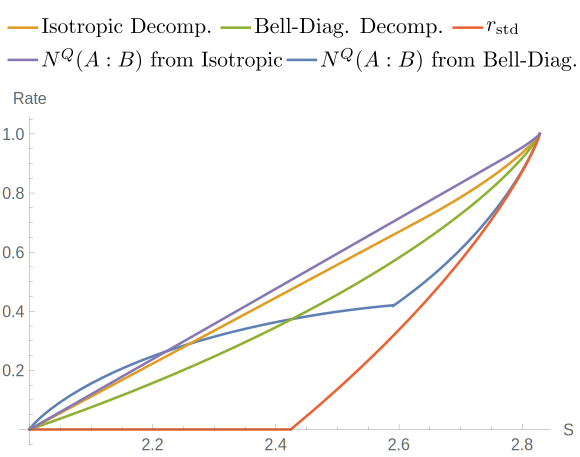
\includegraphics[width=0.7\linewidth]{new_plot.pdf}
      \caption[Comparison of upper bounds for CHSH-based protocols.]{\label{fig:genubound} Upper bounds based on \Cref{eqn:genubound_state} for CHSH-based protocols, with either Bell-diagonal states or isotropic states used in the decomposition. The bounds from quantum intrinsic nonlocality measured on isotropic states~\cite{DIQKD_Limits}, and upper-bounded on Bell-diagonal states~\cite[Appendix B]{RevisedPeres} are plotted for comparison, although note that the quantum intrinsic nonlocality is only proven to be an upper bound for protocols where Alice and Bob broadcast their input settings. (Source:~\cite{CCSquashedEntangle})}
    \end{figure}

    There has been a recent flurry of research related to upper bounds on behaviours~\cite{NotSufficient, RevisedPeres, DIQKD_QKD_Gap, CCSquashedEntangle, DIQKD_Limits}. Fortunately,~\cite{CCSquashedEntangle} unifies most of these results to produce state-of-the-art upper bounds. We modify their notation in order to align it better with our discussion thus far.

    For any arbitrary DIQKD protocol, an upper bound for a specific qqq state and measurement strategy is given by~\cite[Thm. 3]{CCSquashedEntangle}
    \begin{equation}\label{eqn:genubound_state}
    C^{\otimes}_{\sk}(p) \leq \inf_{\substack{\rho,\sM : \\ \behav{\rho}{ \sM} = p}} \inf_{\substack{q : \\ \rho = (1-q)\rho^{NL} + q\rho^L}} (1-q) \inf_{\substack{\sigma^{NL}, \sN : \\ \behav{\sigma^{NL}}{ \sN} \\ = \behav{\rho^{NL}}{ \sM} }} E_R(\sigma^{NL}) + q \inf_{\substack{\sigma^L, \sN : \\ \behav{\sigma^L}{ \sN} \\ = \behav{\rho^L}{ \sM} }} E_R(\sigma^L),
    \end{equation}
  where \(\behav{\rho^L}{ \sM} \in \Ls\) and \(\behav{\rho^{NL}}{ \sM} \not\in \Ls\). Essentially, we decompose the state into local and nonlocal parts (where states are classified as local or nonlocal based on the behaviour produced using the chosen measurement strategy), and compute the relative entropy of entanglement for each part, then minimise over the possible states, measurements and decompositions. Due to the device-independence of the distillation protocol, Eve is free to choose any states and measurements that would not be device-independently distinguishable from the expected states and measurements used in the device.

    While highly general, this bound is extremely difficult to compute, because of the vast, unstructured search space and the nested optimisation, including the optimisation for the relative entropy of entanglement. Fortunately, since all the optimisations are infima, any choice for the parameters is by definition an upper bound, and this bound can be used to evaluate the performance of a protocol on a given implementation. The authors themselves computed this bound only for a specific choice of measurements and states, parametrised by CHSH values, as shown in \Cref{fig:genubound}. Writing \(S\) for \(S_{0101}\) (\Cref{sec:nl_Q}), these states are the \emph{isotropic states} with
    \begin{equation}
      \rho^{I}(v) = v\ket{\Phi_+}\bra{\Phi_+} + \frac{1-v}{4}I
    \end{equation}
    with measurements
    \begin{gather*}
      A_0 = \sigma_3 \qquad A_1 = \sigma_1 \\
      B_0 = \frac{\sigma_3 + \sigma_1}{\sqrt{2}} \qquad B_1 = \frac{\sigma_3 - \sigma_1}{\sqrt{2}} \qquad B_2 = \sigma_3,
    \end{gather*}
    where
    \[ \sigma_1 = \begin{bmatrix} 0 & 1 \\ 1 &  0 \end{bmatrix} \qquad \sigma_3 = \begin{bmatrix} 1 & 0 \\ 0 & -1 \end{bmatrix} \]
    are the \(X\) and \(Z\) Pauli matrices, achieving \(S = 2\sqrt{2}v\), and the decompositions are then accomplished with and \emph{Bell diagonal states} with
    \begin{equation}
      \rho^{\Psi}(C) = \frac{1+C}{2}\ket{\Psi_+}\bra{\Psi_+} + \frac{1-C}{2}\ket{\Psi_-}\bra{\Psi_-},
    \end{equation}
    where the \emph{Bell states} are
    \begin{equation}
      \ket{\Phi_{\pm}} = \frac{1}{\sqrt{2}}\left( \ket{00} \pm \ket{11} \right) \qquad \ket{\Psi_{\pm}} = \frac{1}{\sqrt{2}}\left( \ket{01} \pm \ket{10} \right),
    \end{equation}
    with measurements
    \begin{gather*}
      A_0 = \sigma_3 \qquad A_1 = \sigma_1 \\
    B_0 = \frac{1}{\sqrt{1+C^2}}\sigma_3 + \frac{C}{\sqrt{1+C^2}}\sigma_1 \qquad B_1 = \frac{1}{\sqrt{1+C^2}}\sigma_3 - \frac{C}{\sqrt{1+C^2}}\sigma_1 \\
    B_2 = \sigma_3,
    \end{gather*}
    achieving \(S = 2\sqrt{C^2+1}\). However, these bounds are faithful, at least for the implementations considered.

    The \emph{quantum intrinsic nonlocality} is defined as~\cite{DIQKD_Limits}
    \begin{equation}
    N^Q{(\crv{A}:\crv{B})}_p = \sup_{\prin} \inf_{\rho_{\crv{ABXY}E}\in\compatstates{p}{\prin}} I{(\crv{A}:\crv{B}|\crv{XY}E)}_{\rho}.
    \end{equation}
    \(N^Q{(\crv{A}:\crv{B})}_p\) is an upper bound on a wide range of protocols, including those with two-way information reconciliation, but excluding those where the measurement settings are not revealed. \(N^Q\) was proposed and evaluated on isotropic states with fixed measurements in~\cite{DIQKD_Limits}. For evaluating a CHSH-based protocol, where only the CHSH value, and not the full behaviour, is used to determine the security of the key established, this implementation is outperformed by \Cref{eqn:genubound_state} using either Bell-diagonal or isotropic decompositions, both of which are in turn outperformed by an estimate of \(N^Q\) via the intrinsic information of Bell-diagonal states in~\cite[Appendix B]{RevisedPeres} for \(S \gtrsim 2.43\).

    Observe that, for any fixed \(\rho\),
    \begin{align}
      I{(\crv{A}:\crv{B}|\crv{XY}E)}_{\rho} &= H{(\crv{A}|\crv{XY}E)}_{\rho} - H{(\crv{A}|\crv{BXY}E)}_{\rho} \\
                                            &= \sum_{x,y} \prin(x,y) \underbrace{\left[ H{(\crv{A}|\crv{X}=x,\crv{Y}=y,E)}_{\rho} - H{(\crv{A}|\crv{B},\crv{X}=x,\crv{Y}=y,E)}_{\rho} \right]}_{\geq 0},
    \end{align}
    where the inequality holds by subadditivity of the conditional entropy. If we hold \(\rho\) fixed and allow \(\prin\) to vary, since this is a convex combination of nonnegative terms, the supremum is achieved by a deterministic \(\prin\) that always chooses the inputs \(x\) and \(y\) that give the largest possible conditional mutual information. Therefore, even though this bound is a supremum of an infimum, a looser but still valid upper bound can be computed by fixing the state being sent and selecting the appropriate deterministic \(\prin\).

    We have that \(N^Q{(\crv{A}:\crv{B})}_p = 0 \Leftrightarrow p \in \Ls\)~\cite[Thm 20]{DIQKD_Limits}, that is, the quantum intrinsic nonlocality is a faithful upper bound. Nonetheless, one possible reason for a behaviour outside of \(\Ls\) to have nonzero \(N^Q\) but zero key rate might be that the optimal input behaviour requires the consumption of shared secrecy, which prevents any net increase in key length.

    % NEXT examine proof of faithfulness more carefully, see implications for
    % above argument

    There is thus far only one (possibly) non-faithful upper bound that has been found for quantum adversaries, discussed in~\cite{NotSufficient}. Interestingly, it uses classical information processing to carry out the attack, by proving the existence of a classical strategy for Eve to reduce the conditional mutual information of Alice and Bob to 0, for behaviours that can be obtained by projective measurements on two-qubit \emph{Werner states}\footnote{The two-qubit Werner state can be transformed into the two-qubit isotropic state by applying the \(X\) and \(Z\) Pauli matrices to one party's state, which is a local unitary transformation. More generally, the Bell states can be converted between each other through local unitaries. The Werner states and isotropic states are defined here for only two qubits, but have higher-dimensional generalisations that still retain a connection for them; a recent article studying their structure and their nonlocal properties is~\cite{WernerIsotropicDecomp}.}  with arbitrarily many outcomes.

    Werner states with visibility \(v\)
    \begin{equation}
      \rho^{W}(v) \coloneqq v{\ket{\Psi_-}\bra{\Psi_-}} + \frac{1-v}{4}I,
    \end{equation}
    cannot exhibit nonlocality for \(v < v_L \approx 0.6829\), but can do so for \(v \geq v_{NL} \approx 0.6964\). However, it is shown that for \(v < v_{\crit} \approx 0.7263 > v_{NL}\), any measurement strategy using projective measurements will produce correlations that can be expressed as a convex combination of behaviours that gives \(I(\crv{A}:\crv{B} \downarrow E) = 0\), implying that \(C_{\sk} = 0\) for all such correlations. Since \(v_{NL} < v_{\crit}\), this includes some correlations that exhibit nonlocality. The critical visibility can be increased even further for specific protocols. These behaviours, then, are prospective targets for revival. However, while we are able to specify some behaviours within this set, it is not clear what this set looks like in general. Characterising it might give more insight into how to go about reviving this region.

    \begin{question}
      Can we characterise the quantumly achievable behaviours from Werner states of a given visibility?
    \end{question}

    However, like \(N^Q\), this upper bound applies only to ``standard'' DIQKD protocols where Alice and Bob announce their choice of basis, leaving open the possibility that protocols that do not involve such announcements, such as~\cites{NonstandardProtocol, DIQKD_MeasInputs}[Prot. 2]{DIQKD_FiniteSize}, may be able to achieve positive key rates, so this is not completely conclusive evidence that \(C_{\sk} = 0\) for these behaviours. Some of these protocols have not received much attention since their publication; for example, to our knowledge, the protocol in~\cite{NonstandardProtocol} has not been proved secure against collective attacks, nor has the protocol in~\cite{DIQKD_MeasInputs} been proved secure against general attacks via the EAT\@. The protocol in~\cite[Prot. 2]{DIQKD_FiniteSize} was mentioned in \Cref{sec:diqkd_proto} in the context of correlated input distributions, and is particularly interesting because it provides a detailed finite key analysis with modern proof techniques. Additionally, it removes the requirement for Alice to announce her inputs, allowing it to circumvent this upper bound (although it does not seem to exploit this fact in its proof). Although it demonstrates a positive key rate for Werner states of visibility as low as \(\approx 0.813\), this still does not close the gap to \(v_{NL}\) or even \(v_{\crit}\).

    Therefore, a possible research direction may be to extend these protocols using more recent proof techniques and protocol features, such as two-way information reconciliation, noisy preprocessing, full behaviour constraints, and the input generation mechanism of~\cite[Prot. 2]{DIQKD_FiniteSize}, in an effort to construct an explicit protocol with a non-zero key rate in this region.
    \begin{question}
      Can existing ``nonstandard'' protocols, not covered by the proof of~\cite{NotSufficient}, demonstrate a positive key rate for behaviours shown there to have zero key rate for standard protocols?
    \end{question}

    Many of these bounds were generalised and superseded using the \emph{classical-classical (cc) squashed entanglement} defined in~\cite{CCSquashedEntangle} as
    \begin{equation}
      E^{cc}_{sq}(\rho, \sM, \prin) = \sum_{xy} \prin(x,y) \inf_{\cE_{x,y}} I{(\crv{A} : \crv{B}|E)}_{\cE_{x,y}(\psi^{\rho})},
    \end{equation}
    where \(\cE_{x,y}\) measures \(\psi^\sigma\), the purification of \({\sigma}\), using the POVMs in \(\sM\) corresponding to \(x\) and \(y\), while applying an arbitrary CPTP map to Eve's system. Notably, this function is convex in \(\rho\). This bound for states and measurements yields several different bounds for behaviours that generally improve on previous results. Denoting the key-generating inputs as \((x^{\star},y^{\star})\), the error rate in the key-generating basis as \(Q(p) = p(a\neq{b}|x^{\star}y^{\star})\) and the value of some function corresponding to the LHS of a Bell inequality as \(\hat{S}\), we have
    \begin{align}
    E^{cc,(x^{\star},y^{\star})}_{sq,par}(p) &= \inf_{\substack{\rho, \sM : \\ \hat{S}(p) = \hat{S}(\behav{\rho}{ \sM}) \\ Q(p) = Q(\behav{\rho}{ \sM}) }} E^{cc}_{sq}(\rho, \sM, \delta_{xx^{\star}}\delta_{yy^{\star}}) \\
  E^{cc,(x^{\star},y^{\star})}_{sq,dev}(p) &= \inf_{\substack{\rho, \sM : \\ p = \behav{\rho}{ \sM}}} E^{cc}_{sq}(\rho, \sM, \delta_{xx^{\star}}\delta_{yy^{\star}}) \\
E^{cc}_{sq,dev}(p,\prin) &= \inf_{\substack{\rho, \sM : \\ p = \behav{\rho}{ \sM}}} E^{cc}_{sq}(\rho, \sM, \prin).
    \end{align}

    We define the \emph{lower convex envelope} \(\LCxE{\{f_i\}} = \tilde{f}\) of a set of functions \(\{f_i\}\) as
    \begin{equation}\label{eqn:LCxEdef}
      \tilde{f}(x) = \max\{ f(x) : \forall x, i : f(x) \leq f_i(x) \land f\text{ convex} \},
    \end{equation}
    and compare the bounds and their domains of validity in \Cref{tab:ccsqcomp}.

    \begin{table}
      \begin{Tabular}{| >{\centering}m{\tableline{0.3}}|m{\tableline{0.7}}|}
        \hline
        \( E^{cc,(x^{\star},y^{\star})}_{sq,par} \leq \LCxE{\{I_{AL}, I_{FBL+}\}} \) & For any protocol that uses one key-generating basis and the statistics \(Q\) and \(\hat{S}\), if these statistics can be generated from Werner states with projective measurements, \(I_{AL}\) is an upper bound for intrinsic information computed in~\cite{RevisedPeres}, while \(I_{FBL+}\) is the non-faithful upper bound from~\cite{NotSufficient}. However, \(E^{cc,(x^{\star},y^{\star})}_{sq,par}\) is a convex upper bound for the key rate, and a lower bound for their lower convex envelope, which itself is a convex upper bound for the key rate. \\ \hline
        \( E^{cc,(x^{\star},y^{\star})}_{sq,dev} \leq I_{FBL+} \) & For any behaviour that can be generated from Werner states with projective measurements, and any protocol that broadcasts the input settings, \(I_{FBL+}\) is the non-faithful upper bound from~\cite{NotSufficient}. However, \(E^{cc,(x^{\star},y^{\star})}_{sq,par}\) is a convex upper bound for the key rate, and a lower bound for \(I_{FBL+}\). \\ \hline
      \end{Tabular}
      \caption{\label{tab:ccsqcomp} Comparison between bounds from cc-squashed entanglement and earlier results.}
    \end{table}

    Once again, it is fortunate that all optimisations are infima, because this is a difficult optimisation to compute. Although it was applied to bound a specific set of protocols, it might be interesting to see if it could have more general applicability.

    \begin{question}
      What bounds on general protocols can we achieve using the cc-squashed entanglement?
    \end{question}

    \subsection{Lower Bounds from Quasi-Relative Entropies}\label{sec:diqkd_qre}

    A recent approach to lower bounding the secret key uses semidefinite programming to directly compute lower bounds on \(H{(\crv{A}|E)}_{\rho}\), among all states \(\rho\) compatible with a given behaviour, by directly computing an approximation to the conditional entropy \(H{(\crv{A}|E)}_{\rho}\). Although this technique does not construct an explicit protocol or implementation, it is still a useful theoretical tool for identifying lower bounds.

    The full derivation of this result involves the use of the operator algebra approach to quantum mechanics and spectral theory, which is generally not covered in undergraduate treatments of quantum mechanics and quantum information. An important practical result from their general approach is the extension to bounded infinite-dimensional operators. This has been reviewed (using more elementary methods, without the generality of operator algebras) in \Cref{sec:qretech}, but for this section, we write the expressions in finite-dimensional form, where all spectra are discrete.

    The natural logarithm has the integral representation
    \begin{equation}
      \ln\left(x\right) = \int_{0}^{1} \frac{x-1}{t(x-1) + 1} \dif{t}.\label{eqn:integral_log}
    \end{equation}
    This integral can be approximated by the \(m\)-point \emph{Gauss-Radau quadrature}, which in this case\footnote{In the literature, this quadrature is often defined differently. See \Cref{sec:qretech_grq} for more details.} consists of values \(t_m = 1\), \(w_m = 1/m^2\), and
    \begin{equation}
      \int_{0}^{1} g(t) \dif{t} \approx \sum_{i=1}^m w_i g(t_i),
    \end{equation}
    for some \(g(t)\). The \(t_i \in \ocintv{0}{1}\) are referred to as \emph{nodes}, while the \(w_i > 0\) are \emph{weights}. These nodes and weights are special in that equality is achieved if \(g(t)\) is a polynomial of degree up to \(2m-2\). Notably, however, when applying this approximation to the integral representation in \Cref{eqn:integral_log}, we have an increasing sequence of lower bounds to it. That is,
    \begin{equation}
      r_m(x) \coloneqq \sum_{i=1}^m \frac{w_i(x-1)}{t_i(x-1) + 1} \leq r_{m+1}(x) \leq \ln\left(x\right) \;\forall m \geq 1.
    \end{equation}

    Therefore, we can write the relative entropy as
    \begin{align}
      D(\rho||\sigma) &= \frac{1}{\ln 2} \Tr{\rho \left(\ln\rho - \ln\sigma\right) } \\
                      &= \frac{1}{\ln 2} \Tr{ \sum_{x,y} y \ln\left(\frac{y}{x}\right) \Pi^{(x)}_{\sigma} \Pi^{(y)}_{\rho}  } \label{eqn:finitedim_relent} \\ 
                      &= -\frac{1}{\ln 2} \Tr{ \sum_{x,y} y \underbrace{\ln\left(\frac{x}{y}\right)}_{\geq r_m(x/y)} \Pi^{(x)}_{\sigma} \Pi^{(y)}_{\rho} } \\
                      &\leq -\frac{1}{\ln 2} \Tr{ \sum_{x,y} y \frac{x-y}{t_i(x-y)+y} \Pi^{(x)}_{\sigma} \Pi^{(y)}_{\rho} },
    \end{align}
    where \(x\) and \(y\) are eigenvalues of \(\sigma\) and \(\rho\), and \(\Pi^{(x)}_{\sigma}\) and \(\Pi^{(y)}_{\rho}\) are their respective eigenprojectors, and the inequality direction is flipped since \(y\) is always positive, and so the logarithm is always being multiplied by a negative number.

    The key insight of this method is in observing that this sum can be commuted with the sum over the eigenvalues to obtain the following inequality, which converges to equality as \(m\to\infty\)
    \begin{equation}
      D(\rho||\sigma) \leq - \sum_{i=1}^{m} \frac{w_i}{\ln 2} \underbrace{\Tr{ \sum_{x,y} y \frac{x-y}{t_i(x-y)+y} \Pi^{(x)}_{\sigma} \Pi^{(y)}_{\rho} }}_{\eqqcolon D_{F_{t_i}}(\rho||\sigma)},\label{eqn:re_from_qre}
    \end{equation}
    and that the \emph{quasi-relative entropy} \(D_{F_{t}}(\rho||\sigma)\) can be characterised variationally as
    \begin{equation}
      D_{F_{t}}(\rho||\sigma) = \frac{1}{t} \inf_Z \Tr{ \rho + \rho(Z + Z^{\dagger}) + (1-t)\rho{}Z^{\dagger}Z + t\sigma{}ZZ^{\dagger} }.\label{eqn:qre_var}
    \end{equation}
  This variational expression is of the form \(\Tr{\rho P}\), where \(P\) is a polynomial of operators. As will be seen later, optimisations of this form can be efficiently approximated (with some technical caveats).

If additionally \(\rho \leq \lambda\sigma\) for some \(\lambda \in \R_+\), then the \(i=m\) optimisation can be bounded analytically. We additionally collect the terms that are not multiplied with the optimisation variable \(Z\), removing the \(\Tr{\rho}\) terms from the optimisation and yielding the constant
    \begin{equation}
    c_m(\Tr{\rho}) = \frac{1}{m^2} \frac{\lambda \Tr{\rho}}{\ln 2} - \sum_{i=1}^m \frac{w_i \Tr{\rho}}{t_i \ln 2}.
    \end{equation}
    Further, we have \(\norm{Z} \leq \alpha_i\) in each optimisation, where
    \begin{equation}\label{eqn:qre_bound}
      \alpha_i = \frac{3}{2} \max\left\{\frac{1}{t_i}, \frac{\lambda}{1-t_i}\right\}.
    \end{equation}

    For DIQKD protocols that use a specific input, say \(x^{\star}\), to generate the key, we can apply this analysis to bound the relevant conditional entropy \(H{(\crv{A}|E, \crv{X}=x^{\star})}_{\rho}\) by observing that
    \begin{align*}
      H{(\crv{A}|E)}_{\rho} &= \log d_A - D(\rho_{\crv{A}E}||I_{\crv{A}}\otimes\rho_{E} / d_A) \\
                            &= \log d_A - \Tr{\rho_{\crv{A}E}(\log(\rho_{\crv{A}E}) - \log(I_{\crv{A}}\otimes\rho_{E} / d_A))} \\
                            &= \log d_A - \Tr{\rho_{\crv{A}E}(\log(\rho_{\crv{A}E}) - \log(I_{\crv{A}}\otimes\rho_{E}) + \log d_A)} \\
                            &= -\Tr{\rho_{\crv{A}E}(\log(\rho_{\crv{A}E}) - \log(I_{\crv{A}}\otimes\rho_{E}))} = -D(\rho_{\crv{A}E}||I_{\crv{A}}\otimes\rho_{E}),
    \end{align*}
    where \(d_A\) is the dimension of Alice's system and \(I_A/d_A\) is the state representing a uniform distribution for Alice's system. Further, \(\rho_{\crv{A}E} \leq I_{\crv{A}} \otimes \rho_{E}\), so we have \(\lambda = 1\).

    Then, with \(r\) arbitrary linear constraints on the behaviour, indexed by \(j\)
    \[ \sum_{abxy} c^{(j)}_{abxy} p(ab|xy) \geq v_j, \]
    and recalling that
    \[ p(ab|xy) = \Tr{\rho_{A B E} \left(M_{a|x} \otimes N_{b|y} \otimes I_{E}\right) }, \]
    we can obtain the lower bound:
    \begin{equation}
    \inf_{\substack{\rho: \exists \sM : \\ \behav{\rho}{ \sM} = p}} H{(\crv{A}|E, \crv{X}=x^{\star})}_{\rho} \geq c_m(1) + q_m(p),
    \end{equation}
    where \(q_m(p)\) is given by
    \begin{equation}
      \begin{aligned}[c]
        \inf & \sum_{i=1}^{m-1} \frac{w_i}{t_i \ln 2} \sum_a \Tr{ 
          \rho_{A B E} \left(
            \begin{gathered}
              M_{a|x^{\star}} \otimes I_{B} \otimes \left[ Z_{a,i} + Z_{a,i}^{\dagger} + (1-t_i)  Z_{a,i}^{\dagger}Z_{a,i} \right] \\
              + t_i \left( I_{A B} \otimes Z_{a,i}Z_{a,i}^{\dagger}\right) 
            \end{gathered}
          \right)
        } \\
          \text{s.t.} & \begin{aligned}[t] 
            & \sum_{abxy} c^{(j)}_{abxy} \Tr{\rho_{A B E} \left(M_{a|x} \otimes N_{b|y} \otimes I_{E}\right) } \geq v_j & & \forall 1 \leq j \leq r \\
            & \sum_{a} M_{a|x} = I_{A}, \sum_{b} N_{b|y} = I_{B} & & \forall x, y \\
            & M_{a|x} \succeq 0, N_{b|y} \succeq 0 & & \forall a, b, x, y \\
          & Z_{a,i} Z_{a,i}^{\dagger} \preceq \alpha_i & & \forall a, i \in \dintv{1}{m-1} \\
          & Z_{a,i}^{\dagger} Z_{a,i} \preceq \alpha_i & & \forall a, i \in \dintv{1}{m-1} \\
            & M_{a|x} \in \sB(A), N_{b|y} \in \sB(B), Z_{a,i} \in \sB(E) & & \forall a, b, x, y, i \\
            & \rho_{A B E} \text{ is a valid state} & &
          \end{aligned}
          \end{aligned}
        \end{equation}

        We can use Naimark's dilation theorem to construct a state \(\tilde{\rho}\) and projective measurement operators \(\{\tilde{M}_{a|x}, \tilde{N}_{b|y}\}\) on a Hilbert space \(\Hs\), such that \(\Tr{\tilde{\rho}\tilde{M}_{a|x}} = \Tr{\rho M_{a|x}}\) and  \(\Tr{\tilde{\rho}\tilde{N}_{b|y}} = \Tr{\rho N_{b|y}}\): that is, the behaviour remains the same. These can be mapped to the original behaviour and states via local isometries~\cite{BFF_QRE}.\footnote{See \Cref{sec:ubound_statemeas} for futher detail.} We can further assume that the state is pure, that is, \(\tilde{\rho} = {\ket{\psi}\bra{\psi}}_{\Hs}\), which can only help Eve (due to the data-processing inequality).

        Additionally, instead of enforcing the tensor product explicitly, we can enforce that the operators \(Z_{a,i}\) commute with all \(\tilde{M}_{a|x}\) and \(\tilde{N}_{b|y}\), which in turn commute with each other. Therefore, we can replace all instances of \(\Tr{\rho S}\) in our objective function with \(\braket{\psi|\tilde{S}|\psi}\) for all monomials \(S\) (individual operators and products of operators), where \(\tilde{S}\) is the monomial with all measurements replaced by their projective versions on \(\Hs\). 

        These inner products can then be seen as elements of a Gram matrix for the vectors \(\{\ket{\psi}, \tilde{S}\ket{\psi}\}\), which must be positive semidefinite. In order to constrain \(\ket{\psi}\) to be a valid quantum state, we introduce more vectors of the form \(M\ket{\psi}\), where \(M\) is a monomial formed by the operators in our problem, to our Gram matrix. If all states and operators are valid, the Gram matrix should still be positive semidefinite, no matter the length of the monomials \(M\).

        The \emph{Navascues, Pironio and Acin (NPA) hierarchy} of level \(k\) is the hierarchy that results from including all monomials of length \(k\) in this Gram matrix, which is termed the \emph{moment matrix}~\cite{BoundingQ, ConvHierQ}, while these inner products are termed \emph{moments}. It is a hierarchy of outer approximations to \(\Qs\) that converges, as \(k\to\infty\), to the \emph{almost-quantum set} \(\Qs'\), defined by commuting operators rather than tensor products, and which is strictly larger than \(\Qs\).\footnote{Recent results imply that there is no algorithm that can converge to exactly to \(\Qs\) from outside, since such an algorithm would allow one to solve the halting problem~\cite{MIPRE}. However, if all parties use finite-dimensional systems, \(\Qs = \Qs'\).} Higher levels of the hierarchy involve monomials consisting of longer chains of measurement operators. The NPA hierarchy was later extended to incorporate polynomial operator inequalities by encoding them as \emph{localising matrices}~\cite{NPAHierarchy}, whose entries are linear combinations of the elements of the moment matrix and which must be PSD for the original inequalities to hold.

        The final expression for \(q_m(p)\), which can now be approximated via the NPA hierarchy, is then
        \begin{equation}
          \begin{aligned}[c]
            \inf & \sum_{i=1}^{m-1} \frac{w_i}{t_i \ln 2} \sum_a \angleb{\psi\left|
            \tilde{M}_{a|x^{\star}} \left( Z_{a,i} + Z_{a,i}^{\dagger} + (1-t_i)  Z_{a,i}^{\dagger}Z_{a,i}\right) + t_i Z_{a,i}Z_{a,i}^{\dagger} \right|\psi} \\
              \text{s.t.} & \begin{aligned}[t] 
          & \sum_{abxy} c^{(j)}_{abxy} \angleb{\psi\left| \tilde{M}_{a|x} \tilde{N}_{b|y} \right|\psi} \geq v_j & & \forall 1 \leq j \leq r \\
          & \sum_{a} \tilde{M}_{a|x} = I_{A}, \sum_{b} \tilde{N}_{b|y} = I_{B} & & \forall x, y \\
          & \tilde{M}_{a|x} \succeq 0, \tilde{N}_{b|y} \succeq 0 & & \forall a, b, x, y \\
          & Z_{a,i} Z_{a,i}^{\dagger} \preceq \alpha_i & & \forall a, i \in \dintv{1}{m-1} \\
          & Z_{a,i}^{\dagger} Z_{a,i} \preceq \alpha_i & & \forall a, i \in \dintv{1}{m-1} \\
          & \tilde{M}_{a|x}, \tilde{N}_{b|y}, Z_{a,i} \in \sB(\Hs) & & \forall a, b, x, y, i \\
          & [\tilde{M}_{a|x}, \tilde{N}_{b|y}] = [\tilde{M}_{a|x}, Z_{b,i}] = [\tilde{N}_{b|y}, Z_{a,i}] = 0 & & \forall a, b, x, y, i \\
          & [\tilde{M}_{a|x}, Z_{b,i}^{\dagger}] = [\tilde{N}_{b|y}, Z_{a,i}^{\dagger}] = 0 & & \forall a, b, x, y, i \\
          & \ket{\psi} \text{ is a valid state} & & \\
              \end{aligned}
              \end{aligned}\label{eqn:bff_npa}
            \end{equation}
            The exact translation of these constraints into an SDP is discussed further in \Cref{sec:krwir_wiropt}.

            A few other simplifications are possible, which are discussed and implemented in~\cite{BFF_QRE}:
            \begin{enumerate}
              \item From the normalisation of the measurements, we have that \(\tilde{M}_{o_A|x} = I - \sum_{a < o_A} \tilde{M}_{a|x}\). This allows us to eliminate one measurement operator for each value of \(x\), with the analogous simplification for Bob.
              \item We need only consider inequalities that involve the operators in the objective function, since the other operators can be set to any value without changing the value of the objective function. For a protocol that depends only on the specific input \(x^{\star}\), this means that we need only consider inequalities that involve \(M_{a|x^{\star}}\). Therefore, we need only consider the operators appearing in those inequalities.
              \item We can commute the infimum with the sum. That is, we use the objective function
                \begin{equation} 
                  \sum_{i=1}^{m-1} \inf \frac{w_i}{t_i \ln 2} \sum_a \angleb{\psi\left|
                  \tilde{M}_{a|x^{\star}} \left( Z_{a,i} + Z_{a,i}^{\dagger} + (1-t_i)  Z_{a,i}^{\dagger}Z_{a,i}\right) + t_i Z_{a,i}Z_{a,i}^{\dagger} \right|\psi},
                \end{equation}
                solving \(m-1\) SDPs in sequence. This avoids an optimisation with \((m-1)o_A\) operators \(Z_{a,i}\), which would result in a vastly larger problem that will take much longer to solve. Since the variables in each SDP can be now be varied independently, this can only decrease the infimum computed, thereby decreasing the lower bound on the entropy, but still providing a valid lower bound on the entropy.
              \item The inequality constraints on the operators can be removed in order to speed up the optimisation. Once again, this decreases the value of the achievable infimum, giving a looser but still valid lower bound.
            \end{enumerate}

            \section{Preliminary Results}\label{sec:preres}

            Preliminary results~\cite{KTNotes} found a revival of the standard protocol key rate for states that are generated according to a simple experimental model. We will be using it to illustrate the relevant issues and directions we wish to pursue in our analysis. In this model, we denote the density matrix of Alice's and Bob's quantum state as \(\rho_{AB}\), the dimensions of the Hilbert spaces of their systems \(A\) and \(B\) as \(d_A\) and \(d_B\), and the observables they measure given inputs \(x\) and \(y\) as \(A_x\) and \(B_y\).

            We now model some possible experimental flaws. If our source of quantum states produces one state per time bin, then \(n_c\) is the probability that a state is not produced during a given time bin (where we assume this process to be iid). Further, Alice and Bob's detectors have efficiencies \(\eta_A\) and \(\eta_B\) respectively, which are the probabilities for them to detect a state given that one is produced. If nothing is detected, either due to no signal being produced or due to detector inefficiency, we assign the \(-1\) outcome. The detector failure events are independent, but if no signal is produced, both Alice and Bob will receive no signal.

            We work in Hilbert spaces of dimension \(d_{A} = d_{\tilde{A}} + 1\) and \(d_{B} = d_{\tilde{B}} + 1\), where the states and measurements for a perfect experimental setup have support only on the subspaces of dimension \(d_{\tilde{A}}\) and \(d_{\tilde{B}}\), and the additional subspace is the support of the vacuum state \(\ket{\rm vac}\). We use tildes to denote the states and measurements in the ideal experimental case embedded in this larger Hilbert space. We can then express the overall states and observables as follows:
            \begin{align*}
              A_x &= (1-\eta_A)\tilde{A}_x - \eta_A I_{\tilde{A}} - \ket{\rm vac}\bra{\rm vac}_{A} \\
              B_y &= (1-\eta_B)\tilde{B}_y - \eta_B I_{\tilde{B}} - \ket{\rm vac}\bra{\rm vac}_{B} \\
              \rho_{AB} &= (1-n_c)\tilde{\rho}_{AB} + n_c \ket{\rm vac}\bra{\rm vac}_{A} \otimes \ket{\rm vac}\bra{\rm vac}_{B},
            \end{align*}
            where \(I_{\tilde{A}}\) and \(I_{\tilde{B}}\) are the projectors onto the ideal experiment subspaces.

            The marginals and correlators, then, are as follows:
            \begin{align*}
            \angleb{A_x} &= \Tr{\rho_{AB} A_x \otimes I_A} = -n_c + (1-n_c)(\eta_A\angleb{\tilde{A}_x} - (1-\eta_A)) \\
          \angleb{B_y} &= \Tr{\rho_{AB} I_A \otimes B_y} = -n_c + (1-n_c)(\eta_B\angleb{\tilde{B}_y} - (1-\eta_B)) \\
        \angleb{A_x B_y} &= \Tr{\rho_{AB} A_x \otimes B_y} = \begin{aligned}[c]
      & n_c + (1-n_c)(\eta_A\eta_B\angleb{\tilde{A}_x\tilde{B}_y} - \eta_A(1-\eta_B)\angleb{\tilde{A}_x} \\
      & -\eta_B(1-\eta_A)\angleb{\tilde{B}_y} + (1-\eta_A\eta_B) )
              \end{aligned}
              \end{align*}

              \begin{figure}
                \centering
                \includegraphics[width=0.8\linewidth]{and_plot.pdf}
                \caption{\label{fig:exptplt} Minimum \(\eta\) required for \(r_{\std} > 0\), given \(n_c\). Plotted using \texttt{expt\_wiring\_plot} in \texttt{plots.jl}.}
              \end{figure}

              Consider the following simple wiring, the \emph{N-AND wiring}, where we broadcast the same inputs \(x\) and \(y\) to \(N\) boxes on each side, and drive an AND gate with all the outputs. Clearly, this can only increase the correlation between Alice and Bob, since \(a \neq b\) only if all \(N\) boxes return different outputs to Alice and Bob. However, this means that if Eve knows that any of the boxes produced 0, she can conclude that the overall output is 0, increasing her correlation with Alice. If Alice's increase in correlation with Bob exceeds her increase in correlation with Eve, then this wiring improves the key rate.

              For \(N\) boxes, the correlators and marginals become
              \begin{gather}
                \angleb{A_x B_y}_{N} = 1 - \frac{{(1-\angleb{B_y})}^N + {(1-\angleb{A_x})}^N}{2^{N-1}} + \frac{1}{4^{N-1}} {(1-\angleb{A_x} - \angleb{B_y} + \angleb{A_x B_y})}^{N} \\
                \angleb{A_x}_{N} = 1 - 2 {\left(\frac{1-\angleb{A_x}}{2}\right)}^N \qquad \angleb{B_y}_{N} = 1 - 2 {\left(\frac{1-\angleb{B_y}}{2}\right)}^N,
              \end{gather}
              and we denote the resultant behaviour as \(p_N\).

              Using the standard protocol key rate, we are able to find \emph{revival} in certain parameter regimes: behaviours with \(r_{\std}(p) = 0\), but which have \(r_{\std}(p_N) > 0\), as shown in \Cref{fig:exptplt}. For this plot, we set \(\eta_A = \eta_B = \eta\) and use
              \begin{align*}
                \tilde{A}_x &= \left(\cos\mu_x \sigma_3 + \sin\mu_x \sigma_1\right) \oplus [0] \\
                \tilde{B}_y &= \left(\cos\nu_y \sigma_3 + \sin\nu_y \sigma_1\right) \oplus [0] \\
                \ket{\psi} &= \cos\theta \ket{00} + \sin\theta \ket{11},\,\tilde{\rho}_{AB} = \ket{\psi}\bra{\psi},
              \end{align*}
              where
              \[ \sigma_1 = \begin{bmatrix} 0 & 1 \\ 1 &  0 \end{bmatrix} \qquad \sigma_3 = \begin{bmatrix} 1 & 0 \\ 0 & -1 \end{bmatrix} \]
              are the \(X\) and \(Z\) Pauli matrices on the ideal experimental subspace spanned by \(\{\ket{0}, \ket{1}\}\), and \(\theta=0.15\pi\), \({(\mu_x)}_x = (\pi, 2.53\pi)\), \({(\nu_y)}_y = (2.8\pi, 1.23\pi, \pi)\).

              Based on these observations, it is possible that \(C^{\otimes}_{\sk}(p_N) > C^{\otimes}_{\sk}(p)\). However, it might just be that \(r_{\std}(p) < C^{\otimes}_{\sk}(p)\), and that the wiring does not improve the secret key capacity. We can now state our primary research question more precisely:
              \begin{funqn}\label{fqn:wircap}
                Can local wirings increase the secret key capacity of a behaviour? In particular, can they produce revival of a behaviour with zero secret key capacity?
              \end{funqn}

              From a theoretical standpoint, answering this question would develop our currently limited understanding of the nature of the secret key capacity, and practically, the use of such wirings would be an easily-implemented technique that can squeeze secrecy out of a poorly-functioning system. Our hope for this operation being possible derives from these preliminary results, and the wealth of results on how \emph{quantum} operations can strenghten nonlocal correlations significantly. Some of the seminal results in this area, generally termed \emph{revealing hidden nonlocality}, are:
              \begin{itemize}
                \item States which only produce behaviours in \(\Ls\) for any choice of POVM can, if measured multiple times in sequence, produce nonlocal behaviours (and even maximally violate Bell inequalities)~\cite{HiddenNLAllMeas}.
                \item States can be \emph{super-activated}: \(\rho\) can be local while \(\rho \otimes \rho\) is nonlocal~\cite{SuperActivationBipartite}, and the increase in the violation can be arbitrarily large.
                \item An \(n\)-partite state \(\rho\) is entangled iff there exists a state \(\sigma\) that cannot be used to violate CHSH between a certain pair of players, even after local preprocessing, yet \(\sigma \otimes \rho\) is able to do so~\cite{AllEntangHidden}. This includes entangled states that fall into the latter category. Note that this result is slightly different from super-activation, since the state is in product with another state, rather than a copy of itself, but this is a much stronger result since it applies to \emph{all} entangled states.
              \end{itemize}

              One possible approach considered was to examine the operations used in revealing hidden nonlocality, and to see how closely they can be simulated using classical operations on classical data. While we were unable to do so, we leave this research direction open.
              \begin{question}
                What separates quantum from classical operations? How closely can we approximate quantum effects with classical operations.
              \end{question}

              Lastly, these results have previously been investigated in more detail in~\cite{JanLiThesis}. This work focused on a claimed class of extremal wirings, based on the work in~\cite{ShortEntangleSwap}, and studied their effect on the standard protocol key rate \(r_{\std}\). It was not able to establish that extremal wirings maximise \(r_{\std}\)~\cite[Sec. 7.2]{JanLiThesis}, but was able to establish that certain extremal wirings do not increase it, or are equivalent when the two boxes are iid~\cite[Sec. 7.3]{JanLiThesis}. It also attempted to find a parameter region in a more realistic experimental model where this revival is possible, but was unable to do so~\cite[Sec. 9]{JanLiThesis}. Although this project can be seen as a continuation of~\cite{JanLiThesis}, we wish to broaden our scope to consider the secret key capacity in general, not just for the standard protocol. Further, their extension of the results of~\cite{ShortEntangleSwap} to the QKD setting is incorrect, as we will demonstrate in \Cref{sec:locwir_SPG}. We will therefore refer minimally to this work in the course of our exploration.

              \section{Local Wirings}\label{sec:locwir}

              Before proceeding with our analysis, we must define what we mean by ``wirings''. In other words, we must define our \emph{resource theory}. Our approach is based on that of~\cite{NonclassicalCausation}. Taking inspiration from entanglement theory, which studies entanglement as a resource, a more general resource theory defines a set of \emph{free resources} and a set of \emph{free actions}, and studies how the resources in the theory can be converted between each other using only those free actions and free resources.

              While there has been a recent resurgence of interest in developing resource theories of nonlocality and other unusual quantum phenomena, much of the recent work is too abstract and general to be directly applied by us~\cite{Monotones, TypeIndepLOSR}, or focuses only on \emph{single-copy conversions} using \emph{local operations and shared randomness} (LOSR) as the set of free actions~\cite{NonclassicalCausation, TraceDistNL, NLMeas}, instead of the multiple-copy conversions that wirings perform (with a notable exception discussed in \Cref{sec:wirmono_maxcorr}).

              We generalise existing results on resource theories with LOSR as the set of free actions in order to define and study wirings. In this section, we derive three different mathematical representations of wirings, and use them to better understand the structure of the space of wirings, and how wirings impact the secret key capacity of a behaviour.

                While the definitions and discussions here focus on the bipartite case, as in the rest of this report, they generalise readily to the \(n\)-partite case. For simplicity, we will not discuss this case in detail, but will occasionally mention how this generalisation can be done.

              \subsection{Wiring Distributions}\label{sec:locwir_dist}

              \begin{figure}
                \centering
                \begin{minipage}{0.3\linewidth}
                  \centering
                  \includegraphics{behav.tikz}
                \end{minipage}
                \begin{minipage}{0.6\linewidth}
                  \centering
                  \includegraphics{losr.tikz}
                \end{minipage}
                  \caption[Causal influences in an LOSR operation on a quantum behaviour.]{\label{fig:losr} A generic LOSR operation transforms an initial behaviour \(p(a_0 b_0|x_0 y_0)\), depicted on the left, into a new overall behaviour \(p'(ab|xy)\), using classical preprocessing and postprocessing, and shared randomness, depicted on the right. These diagrams depict the causal influences between the systems in this scenario. Double lines indicate nonclassical causation (in this case, quantum effects). (Adapted from~\cite{NonclassicalCausation})}
                \end{figure}

              Local operations involve each party locally preprocessing his inputs, sending the preprocessed input into the box, then postprocessing the received output to generate an overall output. The preprocessing and postprocessing steps can obviously only use data that is available at the point they are executed, so the most general local operations can be described as~\cite[Def. 4]{LocalTransformations}
              \begin{equation}
                p'(a|x) = \sum_{a_0 x_0} p_o(a|x_0 a_0 x) p(a_0|x_0) p_i(x_0|x).
              \end{equation}
              The conditional probabilities expressing the effect of the local operation can be expressed as a single map:
              \begin{equation}\label{eqn:opmap}
                \chi_A(a x_0 | x a_0) \coloneqq p_o(a|x_0a_0x) p_i(x_0|x) = p_o(a|x_0a_0x) p_i(x_0|x a_0)
              \end{equation}
              where the independence of \(p_i\) from \(a_0\) follows by causality: the production of the input \(x_0\) cannot depend on the value of the output \(a_0\), since the input must be produced before the output is received.

              We emphasise that these are \emph{maps}, not conditional distributions calculated from some joint distribution: the conditional distribution \(p'(x_0|x a_0)\) derived from the joint distribution \(p'(a a_0 x_0|x)\), obtained after applying the operation, will in general depend on \(a_0\). The maps can generally be treated as conditional probabilities, with the operations of summing over events and manipulations using Bayes' rule working similarly, but they are defined independently of the behaviours they act on, and hence an expression like \(\chi(a_0)\) would not be meaningful without specifying the input distribution \(\prin(x)\) and the behaviour acted on \(p(a|x)\).

              Note also that each probability \(p'(a|x)\) is a linear function of the probabilities in the original behaviour \(p(a_0|x_0)\), and so a local operation is a linear map. It is easily verified that convex combinations of local operations are still local operations, and therefore the space of local operations is a convex subset of a vector space.

              LOSR operations\footnote{Note that there are some articles which use a slightly different definition of LOSR, such that \(\chi\) is restricted to a nonconvex subset of \(\Ls\). One such article is~\cite{DIQKD_Limits}, which defines quantum intrinsic nonlocality (\Cref{sec:diqkd_ubehav}) and proves it is monotone under LOSR using the different definition. Fortunately, the result still holds using the definition of LOSR we use. See~\cite[Sec A.2]{NonclassicalCausation} for more details, and a justification for the choice of this definition.} are the extension of local operations to a multipartite setting, where each party applies a local operation, but the choice of local operations between different parties can be correlated via \emph{shared randomness}. Formally, then, the set of \(n\)-partite LOSR operations is the convex hull of all possible \(n\)-times tensor products of \(n\) local operations~\cite{LocalTransformations}.\footnote{The spaces of local wiring distributions for different parties are not the same in general, although one could argue that all of them are subspaces of the version of the set of local operations with the maximal number of outputs and the maximal number of inputs, as per the argument in \Cref{sec:nl_ns}.} This tensor product of convex sets has been studied as the \emph{projective tensor product} in~\cite{AliceBobBanach}, but we do not require such a level of mathematical formality. As a concrete example, bipartite LOSR operations transform \(p(a_0 b_0|x_0 y_0) \mapsto p'(ab|xy)\) using a map \(\chi\)~\cite{NonclassicalCausation}:
              \begin{equation}
                p'(ab|xy) = \sum_{abxy} \chi(abx_0y_0|a_0b_0xy) p(a_0b_0|x_0y_0)
              \end{equation}
              that satisfies the \emph{locality} condition
              \begin{equation}
                \begin{aligned}[c]
                  \chi(abx_0y_0|a_0b_0xy) = \sum_{\lambda} P_{\Lambda}(\lambda) \chi_{A|\lambda}(ax_0|a_0x) \chi_{B|\lambda}(by_0|b_0y),
                \end{aligned}
              \end{equation}
              where \(P_{\Lambda}\) is the distribution of the shared randomness, and \(\chi\) can be interpreted as a behaviour within \(\Ls\), with outputs \((a, x_0)\) and \((b, y_0)\), and inputs \((a_0, x)\) and \((b_0, y)\). Each \(\chi_{A|\lambda}\) and \(\chi_{B|\lambda}\) must also satisfy the \emph{no-retrocausation} conditions:
              \begin{equation}
                \begin{aligned}[c]
                  \chi_{A|\lambda}(x_0|a_0x) &= \chi_{A|\lambda}(x_0|x) \\
                  \chi_{B|\lambda}(y_0|b_0y) &= \chi_{B|\lambda}(y_0|y),
                \end{aligned}
              \end{equation}
              which is equivalent to enforcing that they can be decomposed into preprocessing and postprocessing maps as per \Cref{eqn:opmap}: that is, \(\chi_{A|\lambda}\) and \(\chi_{B|\lambda}\) must be local operations.

              Applying the same analysis to the local operations that constitute a wiring, a wiring of \(c\) boxes would need to generate inputs for the \(c\) boxes, and combine the \(c\) outputs into one output. Therefore, the effect of a \emph{\(c\)-box local operation} is fully specified by the \(c+1\) maps \(\chi(a|\cvec{x}^c\cvec{a}^{c}x)\) and \(\chi(x_j|\cvec{x}^{j-1}\cvec{a}^{j-1}x)\), for \(j \in \dintv{1}{c}\), where there are no constraints on maps besides their cardinalities. We term these \(c\)-box local operations \emph{marginal wirings} and denote the set of marginal wirings as \(\sW\).

              \begin{figure}
                \centering
                \includegraphics{wiring.tikz}
                \caption[Causal influences in a wiring between two iid quantum behaviours.]{\label{fig:wiring} Wirings combine multiple behaviours into one using local operations and shared randomness. We have depicted two iid quantum behaviours here for simplicity; our definitions allow wirings to be applied to any system that can be described by a joint conditional probability (that is, a behaviour).}
            \end{figure}

              The space of \(n\)-partite wirings, which we denote \(\sW^n\), is derived in a similar way to the derivation of LOSR operations, although some care needs to be taken in defining and applying the tensor product of marginal wirings to compute the actual behaviour (see \Cref{sec:locwir_mat}). A bipartite wiring would then produce a new behaviour from \(c\) boxes with an arbitrary joint behaviour \(p^c\) wired together:
              \begin{gather}
                p'(ab|xy) = \sum_{\cvec{a}^c\cvec{b}^c\cvec{x}^c\cvec{y}^c} \chi(ab\cvec{x}^c\cvec{y}^c|\cvec{a}^c\cvec{b}^cxy) p^c(\cvec{a}^c\cvec{b}^c|\cvec{x}^c\cvec{y}^c)\label{eqn:jwirdistdef} \\
                \chi(ab\cvec{x}^c\cvec{y}^c|\cvec{a}^c\cvec{b}^cxy) = \sum_{\lambda} P_{\Lambda}(\lambda) \chi_{A|\lambda}(a\cvec{x}^c|\cvec{a}^cx) \chi_{B|\lambda}(b\cvec{y}^c|\cvec{b}^cy) \label{eqn:mwirdistdef}
              \end{gather}
              where \(\cvec{a}^c = {(a_1, a_2, \ldots, a_c)}^{\rm T}\) is the vector of all the outputs from Alice's boxes that are wired together, with analogous definitions for \(\cvec{b}^c\), \(\cvec{x}^c\) and \(\cvec{y}^c\), with \(x_1\) being the input of the first box Alice interacts with, \(a_1\) being its output, and so forth. We refer to the function \(\chi\) as the \emph{joint wiring distribution}, and \(\chi_{A|\lambda}\) and \(\chi_{B|\lambda}\) as the \emph{marginal wiring distributions}. We additionally write \(p' = \chi[p^c]\) to indicate that \(p'\) is the result of applying the wiring \(\chi\) to the joint behaviour \(p^c\). Now, these distributions are clearly elements of \(\Ls\), with outputs \((a, \cvec{x}^c)\) and \((b, \cvec{y}^c)\), and inputs \((\cvec{a}^{c-1}, x)\) and \((\cvec{b}^{c-1}, y)\). However, not every element of \(\Ls\) is a valid wiring, since the wirings are also constrained by the no-retrocausation conditions, as will be discussed below.

                The definition of wiring application in \Cref{eqn:jwirdistdef} is expressed in terms of \(p^c(\cvec{a}^c\cvec{b}^c|\cvec{x}^c\cvec{y}^c)\), the joint behaviour of the \(c\) boxes. This very general formulation accomodates situations where the individual boxes are not simply iid copies of each other, or where the order of the boxes is \emph{permuted}. For example, if Alice and Bob have boxes described by behaviours \(p_1\) and \(p_2\), Alice could give her first input to \(p_1\) while Bob gives his first input to \(p_2\). For independent boxes, then, we have most generally
                  \begin{equation}
                     p^c(\cvec{a}^c\cvec{b}^c|\cvec{x}^c\cvec{y}^c) = \prod_{j=1}^c p_j(a_jb_{\pi(j)}|x_jy_{\pi(j)}),
                  \end{equation}
                  with \(\pi\) some permutation: that is, the order of inputs and outputs to the wirings is always the same, with any permutation being described by the joint behaviour \(p^c\).

                  Nonetheless, in near-term achievable DIQKD setups, Alice and Bob do not have quantum memories, so they must measure quantum states as soon as they receive them, and are not able to store them to measure later based on the measurement outcomes of states received later. This, together with the iid assumption, justifies our primary focus on \emph{ordered iid joint behaviours} of the form
                  \begin{equation}
                     p^c(\cvec{a}^c\cvec{b}^c|\cvec{x}^c\cvec{y}^c) = \prod_{j=1}^c p(a_jb_j|x_jy_j),
                  \end{equation}
                  where \emph{ordered} refers to the fact that \(\pi\) is the identity permutation, and \emph{iid} to the fact that \(p_j = p\;\forall j\). We denote an ordered iid joint behaviour, consisting of \(c\) copies of a behaviour \(p\), as \(p^{\otimes c}\).

              We turn now to the major constraint on possible wirings, namely the no-retrocausation conditions. They are more complex for wirings than in the case of LOSR operations, since later boxes can depend on the output of earlier boxes. If Alice and Bob interact with their boxes in increasing order of the index \(j\), we have the following constraints on quantities derived from summing \(\chi_{A|\lambda}\) and \(\chi_{B|\lambda}\) over \(\cvec{x}^{j+1:c}\) and \(\cvec{y}^{j+1:c}\) respectively:
              \begin{equation}
                \begin{aligned}[c]
                  \chi_{A|\lambda}(\cvec{x}^j|\cvec{a}^cx) &= \chi_{A|\lambda}(\cvec{x}^j|\cvec{a}^{j-1}x),\,\forall j \in \dintv{1}{c} \\
                  \chi_{B|\lambda}(\cvec{y}^j|\cvec{b}^cy) &= \chi_{B|\lambda}(\cvec{y}^j|\cvec{b}^{j-1}y),\,\forall j \in \dintv{1}{c}.
                \end{aligned}\label{eqn:wiringnoretro}
              \end{equation}

            We verify that conditional distributions obeying the no-retrocausation conditions can be decomposed as a sequence of maps using Bayes' rule:
                \begin{align}
                  \chi_{A|\lambda}(a\cvec{x}^c|\cvec{a}^cx) &= \chi_{A|\lambda}(a|\cvec{x}^c\cvec{a}^cx) \chi_{A|\lambda}(\cvec{x}^{c}|\cvec{a}^cx) \\
                                                         &= \chi_{A|\lambda}(a|\cvec{x}^c\cvec{a}^cx) \chi_{A|\lambda}(x_c|\cvec{x}^{c-1}\cvec{a}^cx) \chi_{A|\lambda}(\cvec{x}^{c-1}|\cvec{a}^cx) \\
                                                         &= \chi_{A|\lambda}(a|\cvec{x}^c\cvec{a}^cx) \prod_{j=1}^c \chi_{A|\lambda}(x_j|\cvec{x}^{j-1}\cvec{a}^cx) \\
                                                         &= \chi_{A|\lambda}(a|\cvec{x}^c\cvec{a}^{c}x) \prod_{j=1}^c \chi_{A|\lambda}(x_j|\cvec{x}^{j-1}\cvec{a}^{j-1}x),
                \end{align}
                where in the last line we have used the no-retrocausation conditions in \Cref{eqn:wiringnoretro}. That any such collection of probabilistic maps can be combined into a single distribution can be shown with a calculation similar to that in \Cref{eqn:opmap}.

              Physically, a probabilistic wiring must actually execute some deterministic wiring, and its joint wiring distribution is then a convex combination of the deterministic joint wiring distributions, of which there are finitely many. This is the intuition behind the proof of Fine's theorem presented in~\cite{BellNonlocality}, which can be straightforwardly adapted to \(\sW^n\). Informally, we can express a wiring distribution as a convex combination of marginal wiring distributions, and these marginal wirings can be decomposed further into convex combinations of ``more deterministic'' marginal wiring distributions, offloading the indeterminism they contain into an auxiliary random variable, and redefining \(\lambda\) to incorporate this auxliary variable.
              \begin{theorem}[Fine's Theorem for Wirings]
                The set of marginal wirings \(\sW\) forms a polytope, whose vertices are the set of deterministic marginal wirings obeying the no-retrocausation relations \(\sW_D\). All \(n\)-partite wirings are then elements of the polytope generated by the vertices \(\sW_D^n\).
              \end{theorem}
              \begin{proof}
                Consider a marginal wiring \(\chi_{A|\lambda}\), decomposed into the maps that it applies:
                \begin{equation}\label{eqn:mapdecomp}
                  \chi_{A|\lambda}(a\cvec{x}^c|\cvec{a}^cx) = \chi_{A|\lambda}^{(c+1)}(a|\cvec{x}^c\cvec{a}^{c}x) \prod_{j=1}^c \chi_{A|\lambda}^{(j)}(x_j|\cvec{x}^{j-1}\cvec{a}^{j-1}x),
                \end{equation}
                and denote each map abstractly as \(\chi_{A|\lambda}^{(j)}(t^{(j)}|s^{(j)})\).
                Select a particular \(k\in\dintv{1}{c+1}\), \(\hat{t}^{(k)}\) and \(\hat{s}^{(k)}\) such that \(\chi_{A|\lambda}^{(k)}(\hat{t}^{(k)}|\hat{s}^{(k)}) = 0 < q < 1\). If no such values exist, the wiring is already deterministic, and we are done.
                Now, consider wirings \(\chi_{A|\lambda,0}\) and \(\chi_{A|\lambda,1}\), such that
                \begin{align*}
                  \chi^{(k)}_{A|\lambda,0}(t^{(k)}|\hat{s}^{(k)}) &= \begin{cases}
                    0 & \text{ if } t^{(k)} = \hat{t}^{(k)} \\
                    \frac{1}{1-q} \chi_{A|\lambda}^{(k)}(t^{(k)}|\hat{s}^{(k)}) & \text{ otherwise,} \\
                  \end{cases} \\
                      \chi^{(j)}_{A|\lambda,0}(t^{(j)}|\hat{s}^{(j)}) &= \chi_{A|\lambda}^{(j)}(t^{(j)}|\hat{s}^{(j)}) \text{ otherwise,} \\
                    \chi^{(k)}_{A|\lambda,1}(t^{(k)}|\hat{s}^{(k)}) &= \begin{cases}
                      1 & \text{ if } t^{(k)} = \hat{t}^{(k)} \\
                      0 & \text{ otherwise,} \\
                    \end{cases} \\
                      \chi^{(j)}_{A|\lambda,1}(t^{(j)}|\hat{s}^{(j)}) &= \chi_{A|\lambda}^{(j)}(t^{(j)}|\hat{s}^{(j)}) \text{ otherwise.} \\
                    \end{align*}
                    It is easily verified that both \(\chi_{A|\lambda,0}^{(k)}(t^{(k)}|s^{(k)})\) and \(\chi_{A|\lambda,1}^{(k)}(t^{(k)}|s^{(k)})\) are valid maps, and hence \(\chi_{A|\lambda,0}\) and \(\chi_{A|\lambda,1}\) are valid marginal wiring distributions. Then, we have \(\chi_{A|\lambda} = (1-q)\chi_{A|\lambda,0} + q\chi_{A|\lambda,1}\). We can repeat this process recursively on \(\chi_{A|\lambda,0}\) and \(\chi_{A|\lambda,1}\) until \(\chi_{A|\lambda}\) is decomposed completely into a weighted sum of deterministic wiring distributions
                    \[ \chi_{A|\lambda} = \sum_{w=1}^m q_w \chi_{A|\lambda,w}. \]

                    Then, we define a discrete random variable \(\Lambda' = (\lambda, w)\), where \(w \in \dintv{1}{m}\), with pmf \(P_{\Lambda'}(\lambda, w) = q_w P_{\Lambda}(\lambda)\). Finally, we rewrite our joint wiring distribution\footnote{For concreteness and simplicity of notation, we restrict ourselves to \(n=2\). The proof generalises readily to \(n>2\).} as
                    \begin{equation}
                      \chi(ab\cvec{x}^c\cvec{y}^c|\cvec{a}^c\cvec{b}^cxy) = \sum_{\lambda w} P_{\Lambda'}(\lambda) \chi_{A|\lambda,w}(a\cvec{x}^c|\cvec{a}^cx) \chi_{B|\lambda}(b\cvec{y}^c|\cvec{b}^cy),
                    \end{equation}
                    where now all \(\chi_{A|\lambda,w}\) are deterministic. The same process can be used to decompose Bob's, or any other party's, marginal wiring distribution into a convex combination of deterministic wirings.

                    This demonstrates the sufficiency of deterministic marginal wirings for generating all wirings. To see that all these wirings are necessary, note that, given two distinct deterministic wirings \(\chi_{A|1}\) and \(\chi_{A|2}\), there must be at least one \(s\) and one \(t\) for the wiring distributions, such that \(\chi_{A|1}(s|t) = 0\) and \(\chi_{A|2}(s|t) = 1\). Then, if attempting to express \(\chi_{A|1}\) as a convex combination, where \(\chi_{A|2}\) has a nonzero weight \(q\), and grouping all other distributions in the combination into \(\chi_{A|3}\), we will have \(\chi_{A|1}(s|t) = q\chi_{A|2}(s|t) + (1-q)\chi_{A|3}(s|t) \geq q > 0\), which is a contradiction.
                  \end{proof}

              We refer to the discrete set of deterministic marginal wirings as \(\sW_D\), which are therefore the vertices of the polytope \(\sW\). \(\sW^n\) is then the convex polytope with vertices \(\sW_D^n = \underbrace{\sW_D \times \sW_D \times \cdots \times \sW_D}_{n\text{ times}}\). We also define \(\sWB(p)\) as the set of behaviours generated by applying \(\sW^n\) to an \(n\)-partite behaviour \(p\) using \Cref{eqn:jwirdistdef}.

              Having established this crucial result about the structure of the space of wirings, we can start examining this structure more explicitly, and attempting to find a computationally tractable representation for it that can be applied to analysing DIQKD.

              \subsection{Wiring Functions}\label{sec:locwir_func}

              In order to determine the polytope of joint wirings, we can use the same approach as is typically used for \(\Ls\): enumerate \(\sW_D\), the vertices of \(\sW\), combinatorically, and find the facet-defining inequalities from that list using a facet-enumeration algorithm. The naive implementation would be to enumerate all possible LD behaviours of the correct cardinality and prune them by removing those that violate the no-retrocausation conditions. This brute-force enumeration is implemented in the \verb`LDWiringIter` type in \verb`wiring.jl`. Howwever, we would then have to process \({(o_A i_A^c)}^{i_A^c o_A} {(o_B i_B^c)}^{i_B^c o_B}\) LD behaviours (\(\approx \num{5.12e18}\) for the QKD setting), which is not scalable.

              An alternative approach would be to analyse the wirings in \(\sW_D\) to see if the wiring distribution description contains any redundancies. We use a different, more operational description for deterministic wirings, based on the decomposition into maps that describe the operation of the wiring in \Cref{eqn:mapdecomp}, in order to detect some of these redundancies.  For deterministic wirings, we can consider Alice's inputs \(\cvec{x}^c\) to her boxes as being computed by a sequence of \(c\) deterministic functions with range \(\dintv{1}{i_A}\):
              \begin{equation} x_j = W^{(j)}_{A}(\cvec{x}^{j-1}, \cvec{a}^{j-1}, x),\,j \in \dintv{1}{c} \end{equation}
              and an output function with range \(\dintv{1}{o_A}\):
              \begin{equation} a = T_{A}(\cvec{x}^{c}, \cvec{a}^{c}, x). \end{equation}
              We refer to each function \(W_{A}^{(j)}\) as a \emph{wiring input function}, and \(T_{A}\) as the \emph{wiring output function}, all of these functions as \emph{wiring map functions}, and the overall function representing their composition as a \emph{wiring function}. The corresponding marginal wiring distribution \(\chi_{A}\) is then
              \begin{equation}
                \chi_{A}(a\cvec{x}^c|\cvec{a}^cx) = \indic{a = T_{A}(\cvec{x}^{c}, \cvec{a}^{c}, x)} \prod_{j=1}^c \indic{x_j = W^{(j)}_{A}(\cvec{x}^{j-1}, \cvec{a}^{j-1}, x)}.
              \end{equation}
              The analogous definitions for Bob hold with the appropriate changes of labels \(A \mapsto B\), \(x \mapsto y\), \(a \mapsto b\). Probabilistic wirings can then be described as convex combinations of such deterministic wirings.

              In order to reduce ambiguity, we refer to each wiring map function as mapping a \emph{source}, its argument, to a \emph{target}, its value, reserving ``input'' and ``output'' to describe the inputs and outputs of boxes. Simple combinatorics gives us \(i_A^{j} o_A^{j-1}\) possible sources for \(W^{(j)}_{A}\). However, since the wiring is deterministic, \(x_j\) is completely fixed by \(\cvec{x}^{j-1}\), \(\cvec{a}^{j-1}\) and \(x\). Therefore, when considering each map as part of the overall wiring, the only free choice in the source is \(x\), and so there are only \(i_A o_A^{j-1}\) valid sources.

              \begin{table}
                \begin{minipage}{0.5\linewidth}
                  \begin{center}
                    \begin{tabular}{|r|cc|} \hline
                      \diagbox{\(x x_1\)}{\(a_1\)} & 0 & 1 \\ \hline
                      00 & 1 & 0 \\
                      01 & X & X \\
                      11 & 1 & 1 \\
                      10 & X & X \\ \hline
                    \end{tabular}
                  \end{center}
                \end{minipage}
                \begin{minipage}{0.5\linewidth}
                  \begin{center}
                    \begin{tabular}{|r|cccc|} \hline
                      \diagbox{\(x x_1 x_2\)}{\(a_1 a_2\)} & 00 & 01 & 11 & 10 \\ \hline
                      000 & X & X & 1 & 0 \\
                      001 & 0 & 0 & X & X \\
                      011 & X & X & X & X \\
                      010 & X & X & X & X \\
                      110 & X & X & X & X \\
                      111 & 1 & 0 & X & X \\
                      101 & X & X & X & X \\
                      100 & X & X & 0 & 0 \\ \hline
                    \end{tabular}
                  \end{center}
                \end{minipage}
                \caption[Lookup tables for a specific wiring.]{Left: Lookup table for \(W_{A}^{(2)}\), giving \(x_2\). Right: Lookup table for \(T_{A}\), giving overall output \(a\). Entries forbidden by earlier wirings are marked with X (don't care). Both are written as Karnaugh maps, with the row and column labels in Gray code order.}\label{tab:wiring_lut}
              \end{table}

              Therefore, the number of possibilities for the \(j\)th wiring input function \(W^{(j)}_{A}\) is \(\exp_{i_A}(i_A o_A^{j-1})\). Similarly, the number of possible wiring output functions \(T_{A}\) is \(\exp_{o_A}(i_A o_A^{c})\). The number of distinct elements of \(\sW_D\) is then reduced to
              \begin{equation}
                \exp_{o_A}(i_A o_A^c) \prod_{j=1}^c \exp_{i_A}(i_A o_A^{j-1}).
              \end{equation}
              The same applies to Bob with the appropriate changes of labels \(A \mapsto B\), \(x \mapsto y\), \(a \mapsto b\). 

              A concrete example can help explain this simplification. The deterministic wiring characterised by
              \begin{equation}
                x_1 = x \qquad x_2 = \bar{a}_1 + x_1 \qquad a = x_1x_2\bar{a}_1\bar{a}_2 + \bar{x}_1\bar{x}_2a_1a_2\label{eqn:wiringeg}
              \end{equation}
              is represented by the lookup tables in~\Cref{tab:wiring_lut}, where juxtaposition is the Boolean AND, addition is the Boolean OR, and the overbar is the Boolean NOT.\ \(W_{A}^{(2)}\) and \(T_{A}\) are fully specified by 4 and 8 values respectively, instead of the full 8 and 32 values that would be needed to specify the target for each source sequence.

              Another way to reduce the number of wirings would be to fix some input settings to use a given wiring. For example, if both parties apply the AND gating to specific inputs, the correlators involving those inputs will increase in value. Therefore, we can fix the key generating settings \(x = 1\) and \(y = 3\) to be AND-wired. If we fix the wirings for \(f\) input settings, then the number of possible sources for the \(j\)th function will be \((i_A - f) o_A^{j-1}\), so the number of possible wirings becomes
              \begin{equation}
                \exp_{o_A}((i_A-f) o_A^c) \prod_{j=1}^c \exp_{i_A}((i_A-f) o_A^{j-1})
              \end{equation}
              for Alice, with the analogous relabelling for Bob.

              This iteration is implemented as the \verb`WiringFnIter` type in \verb`wiring.jl`, which allows the maps to fix to be specified. For the case of two boxes in the QKD setting, there are 16384 marginal wiring functions for Alice, and \(\approx \num{8.06e7}\) for Bob, for a total of \(\approx \num{1.32e12}\) joint wiring functions. Fixing the AND gating as discussed above gives us 128 marginal wiring functions for Alice and 186624 for Bob, for a total of \(\approx \num{2.39e7}\) joint wiring functions. Both are much more manageable than the number of vertices of \(\Ls\) without causality constraints, but still a substantial computational workload.

              \subsection{Wiring Matrices}\label{sec:locwir_mat}

              Inspired by the analysis of single-copy local transformations in~\cite{LocalTransformations}, another approach would be to view each wiring map function as a reversible symmetry operation on its source, followed by an irreversible mapping to a target, and then a reversible symmetry operation on the target. We can simplify our analysis using the observation that the symmetry operations on the target of one wiring map function are of the same type as the symmetry operations on the source of the subsequent wiring map function. Let \(S\) be a symmetry operation on the source of a wiring map function, \(T\) the symmetry operation on the target of a function, and \(R\) the irreversible operation implemented by the wiring map function. Then, the overall effect of a wiring on a behaviour \(p\) can be informally expressed as
              \[ T_{c+1}R_{c+1}S_{c+1} \cdots T_2R_2S_2 T_1R_1S_1 p. \]
              Our argument then is that \(S_{j+1}\) and \(T_{j}\) for any \(j\) are elements of the same group of transformations, and can therefore be combined when enumerating the possible deterministic transformations. The sequence of operations is then effectively
              \[ R_{c+1}S_{c+1} \cdots R_2S_2 R_1S_1 p, \]
              where we have dropped the final symmetry operation \(T_{c+1}\) because, as will be demonstrated later, it does not perform any transformation that variation in the other operators cannot produce.

              We will formalise this by expressing the wirings as linear operators: that is, matrices. Since the deterministic marginal wirings are local, they are entirely characterised by their effect on a single-party behaviour, with the effect of a joint deterministic wiring being isomorphic to that of the tensor product of the marginal wirings, as explicitly described later in this section. While our examples, explanations and implementations focus primarily on ordered iid joint behaviours (\Cref{sec:locwir_dist}), they are straightforwardly extended to more general joint behaviours.

              We first consider the case of a single party, whose box takes input \(x \in \dintv{1}{i_A}\) and gives output \(a \in \dintv{1}{o_A}\). We vectorise the behaviour by incrementing \(a\), then \(x\), that is
              \begin{equation}
                \matr[_A]{p}_k = p(a|x) \Leftrightarrow k = (a-1) i_A + x,
              \end{equation}
              which means that \(\cvec{p}_A\), the vector corresponding to the behaviour, is the direct sum of normalised probability vectors \(\cvec{p}_{A|x}\), each corresponding to the distribution obtained from input \(x\). We refer to the real vector space that \(\cvec{p}_A\) lives in as \(\sP_A \cong \R^{o_Ai_A}\).

              We want to represent the wiring of \(c\) independent boxes together as the action of a matrix \(\matr[_A]{W}\) on \(\cvec{p}_A^{\otimes c}\). Further, we want to represent each wiring map function as a matrix \(\matr[_A^{(j)}]{W}\) (or \(\matr[_A]{T}\) for the wiring output function), acting on a single-party behaviour representing the box being wired, and the auxiliary information collected thus far. This state information is represented as a vector \(\cvec{p}^{(j)}_A\), and we want
              \[ \matr[_A]{W} = \matr[_A]{T} \matr[_A^{(c)}]{W} \matr[_A^{(c-1)}]{W} \cdots \matr[_A^{(1)}]{W}. \]
              To additionally represent the dependency on the overall input \(x\), the initial state of the system must be an element of \(\R^{i_A} \otimes \sP_A^{\otimes c}\). Therefore, we have
              \begin{equation}
                \cvec{p}_A^{(1)} = \bigoplus_{l=1}^{i_A} 1 \otimes \bigotimes_{k=1}^c \cvec{p}_A.
              \end{equation}

              Now, application of a wiring map function, aside from the output function \(T_A\), corresponds to performing a wiring, inputting the wiring map function's target into the next nonlocal box, and then retrieving the nonlocal box output. However, we do not need to record the wiring map function's target, as argued in \Cref{sec:locwir_func}; we only need the box output that will become part of the next wiring map function's source. Therefore, we can have
              \[ \matr[_A^{(1)}]{W} \cvec{p}_A^{(1)} = \cvec{p}_A^{(2)} \in \R^{i_A} \otimes \R^{o_A} \otimes \sP_A^{\otimes c-1}, \]
              which we can generalise to
              \begin{equation}
                \matr[_A^{(j)}]{W} \cvec{p}_A^{(j)} = \cvec{p}_A^{(j+1)} \in \R^{i_A} \otimes \bigotimes_{k=1}^{j} \R^{o_A} \otimes \bigotimes_{l=1}^{c-j} \sP_A,\, \forall j \in \dintv{1}{c}.
              \end{equation}
              The matrix \(\matr[_A^{(j)}]{W}\) depends on \(\R^{i_A}\) and all existing copies of \(\R^{o_A}\), but maps only one copy of \(\sP_A\) to one copy of \(\R^{o_A}\) and leaves the values in \(\R^{i_A}\) and the copies of \(\R^{o_A}\) unchanged. That is, we can write the matrix as
              \begin{equation}
                \matr[_A^{(j)}]{W} = \matr[_A^{(j)}]{\tilde{W}} \otimes \bigotimes_{l=1}^{c-j} I_{\sP_A} \, \forall j \in \dintv{1}{c},
              \end{equation}
              where the matrices \(\matr[_A^{(j)}]{\tilde{W}}\) are maps from \(\R^{i_A} \otimes \bigotimes_{k=1}^{j-1} \R^{o_A} \otimes \sP_A\) to \(\R^{i_A} \otimes \bigotimes_{k=1}^{j} \R^{o_A}\). \(\matr[_A]{T}\) is, however, a map from \(\R^{i_A} \bigotimes_{k=1}^{c} \R^{o_A}\) to \(\sP_A\), and does not admit such a factorisation.

              The matrices \(\matr[_A^{(j)}]{\tilde{W}}\) can be factorised into a \emph{permutation map} \(\matr[_A^{(j)}]{S}\) (i.e.\ a symmetry operation) followed by an \emph{application map} \(\matr[_A^{(j)}]{R}\), corresponding respectively to \(S_j\) and \(R_j\) for \(j \leq c\) in our informal notation. However, both maps must be a direct sum of \(i_A\) smaller \emph{conditional submatrices}, in order to preserve the separation between the \(i_A\) possible values of the overall input \(x\). This separation must be preserved throughout for the output matrix \(\matr[_A]{T}\), which also consists of a permutation map \(\matr[_A^{(j)}]{S}\) and application map \(\matr[_A]{T}\) that are direct sums of conditional submatrices, to be able to correctly assign the probabilities based on the overall input \(x\). Therefore, we have
              \begin{align}
                \matr[_A^{(j)}]{W} &= \left( \bigoplus_{x=1}^{i_A} \matr[_{A|x}^{(j)}]{R} \right) \left( \bigoplus_{x=1}^{i_A} \matr[_{A|x}^{(j)}]{S} \right) \\
                                   &= \matr[_{A}^{(j)}]{R} \matr[_{A}^{(j)}]{S} \\
                \matr[_A]{T} &= \left( \bigoplus_{x=1}^{i_A} \matr[_{A|x}]{T} \right) \left( \bigoplus_{x=1}^{i_A} \matr[_{A|x}^{(c+1)}]{S} \right) \\
                                   &= \matr[_{A}]{T} \matr[_{A}^{(c+1)}]{S}.
              \end{align}

              Each application matrix \(\matr[_{A}^{(j)}]{R}\) can be considered abstractly as mapping each source sequence \(\cvec{a}^{j-1}\) to a specific value of \(x_j\), and multiplying the probability of the source sequence with \(\cvec{p}_{A|x_j}\). In order to operate on a copy of \(\cvec{p}_A\), the conditional submatrix \(\matr[_{A|x}^{(j)}]{R}\) for a given \(x\) must take the following form:
              \begin{equation}
                \matr[_{A|x}^{(j)}]{R} = \left( \bigoplus_{l=1}^{n_1} \underbrace{\begin{bmatrix} 1 & 0 & 0 & \cdots \end{bmatrix}}_{i_A\text{ entries}}
                  \oplus \bigoplus_{l=1}^{n_2} \underbrace{\begin{bmatrix} 0 & 1 & 0 & \cdots \end{bmatrix}}_{i_A\text{ entries}} \oplus \cdots
                \right) \otimes I_{o_A},
                \end{equation}
                where \(n_l\) is the number of source sequences \(\cvec{a}^{j-1}\) mapped to \(x_j = l\). The matrices in the direct sum of matrices identify a particular value of \(x\), and \(I_{o_A}\) maps the respective \(\cvec{p}_{A|x}\) to \(\R^{o_A}\). The enumeration of the application matrices then reduces to a ``stars and bars'' combinatorics problem: each tuple of non-negative integers \({(n_k)}_{k=1}^{i_A}\) such that \( \sum_{k} n_k = o_A^{j-1} \) corresponds to a unique application matrix. This is equivalent to selecting \(i_A-1\) slots out of \(o_A^{j-1}+i_A-1\) as ``bars'', and placing the source sequences (the ``stars'') into the remaining \(o_A^{j-1}\) slots in a fixed order. The ``bars'' then divide the ``stars'' into \(i_A\) possibly empty bins, as required. Therefore, there are \(\binom{o_A^{j-1} + i_A-1}{i_A-1}\) possible application matrices.

                While the application matrix determines the multiplicity of each input, the permutation matrix takes care of assigning the source sequences to those inputs. It is a permutation matrix, consisting of the identity matrix with its rows permuted, with a tensor product with \(I_{i_A o_A}\) in order to operate on the probabilities \(\cvec{p}\). However, there are degeneracies here as well. The number of permutations with different effects can be calculated by considering the combinatoric problem of assigning \(n_1\) inputs \(1\), \(n_2\) inputs \(2\), and so on, to \(o_A^{j-1}\) source sequences. There are therefore \(o_A^{j-1}!/\prod_{k=1}^{i_A} n_k!\) possible permutation matrices.

                \(\matr[_A]{T}\) maps an element of \(\R^{i_A} \otimes \bigotimes_{k=1}^{c} \R^{o_A}\) to \(\sP_A\). Analogous to the case of \(\matr[^{(j)}_A]{W}\), the application matrix provides the multiplicity of output values, while the permutation matrix decides which probabilities are assigned to which output. This gives \(\binom{o_A^c + o_A-1}{o_A-1}\) application matrices and \(o_A^c!/\prod_{k=1}^{o_A} n_k!\) permutation matrices. From this analysis, it is clear that the final output permutation would not generate any permutation that would not already be generated by \(\matr[_A^{(c+1)}]{S}\), and hence can be safely removed.

                For clarity, we provide an explicit example using the wiring characterised by \Cref{eqn:wiringeg}, and define \(\cvec{\tilde{p}}_A^{(j)}\) as the element of \(\R^{i_A} \otimes \bigotimes_{k=1}^{j-1} \R^{o_A} \otimes \sP_A\) that is acted on by \(\matr[_A^{(j)}]{\tilde{W}}\). To improve readability, we have also factorised out tensor products with identity matrices. The effect of the wiring can then be written as:
                \begin{align}
                  \matr[_A^{(1)}]{\tilde{W}} \cvec{\tilde{p}}{_A^{(1)}} &= \left( \left(
                      \begin{bmatrix} 1 & 0 \\ \end{bmatrix} 
                  \oplus \begin{bmatrix} 0 & 1 \\ \end{bmatrix} \right) \otimes I_2 \right)
                  \left( \left( \begin{bmatrix} 1 \end{bmatrix} \oplus \begin{bmatrix} 1 \end{bmatrix} \right) \otimes I_{4} \right) 
                  \left( \begin{bmatrix} 1 \\ 1 \end{bmatrix} \otimes \cvec{p}_A \right) \\
                                           &= \begin{bmatrix}
                                             I_2 & 0_{2\times 2} & 0_{2\times 2} & 0_{2\times 2} \\
                                             0_{2\times 2} & 0_{2\times 2} & 0_{2\times 2} & I_2 \\
                                             \end{bmatrix} I_{8} \begin{bmatrix}
                                             \cvec{p}_{A|0} \\
                                             \cvec{p}_{A|1} \\
                                             \cvec{p}_{A|0} \\
                                             \cvec{p}_{A|1} \\
                                             \end{bmatrix} = \begin{bmatrix}
                                             \cvec{p}_{A|0} \\
                                             \cvec{p}_{A|1} \\
                                           \end{bmatrix} \in \R^{i_A} \otimes \R^{o_A} \\
                  \matr[_A^{(2)}]{\tilde{W}} \cvec{\tilde{p}}{_A^{(2)}} &= \begin{gathered}
                    \left( \left(
                        \left( \begin{bmatrix} 1 & 0 \\ \end{bmatrix} \oplus \begin{bmatrix} 0 & 1 \\ \end{bmatrix} \right)
                    \oplus \bigoplus_{k=1}^2 \begin{bmatrix} 0 & 1 \\ \end{bmatrix} \right) \otimes I_2 \right) \\
                    \left( \left( \begin{bmatrix} 0 & 1 \\ 1 & 0 \\ \end{bmatrix} \oplus
                    \begin{bmatrix} 1 & 0 \\ 0 & 1 \\ \end{bmatrix} \right) \otimes I_{4} \right)
                    \left( \begin{bmatrix} \cvec{p}_{A|0} \\ \cvec{p}_{A|1} \end{bmatrix} \otimes \cvec{p}_A \right) \end{gathered} \\
                                      &=
                                      \begin{bmatrix}
                                        \begin{bmatrix} I_2 & 0_{2\times{2}} \\ \end{bmatrix} & 0_{2\times{4}} & 0_{2\times{4}} & 0_{2\times{4}} \\
                                        0_{2\times{4}} & \begin{bmatrix} 0_{2\times{2}} & I_2 \\ \end{bmatrix} & 0_{2\times{4}} & 0_{2\times{4}} \\
                                        0_{2\times{4}} & 0_{2\times{4}} & \begin{bmatrix} 0_{2\times{2}} & I_2 \\ \end{bmatrix} & 0_{2\times{4}} \\
                                        0_{2\times{4}} & 0_{2\times{4}} & 0_{2\times{4}} & \begin{bmatrix} 0_{2\times{2}} & I_2 \\ \end{bmatrix} \\
                                      \end{bmatrix}
                                      \begin{bmatrix} 
                                        p(1|0) \cvec{p}_A \\ p(0|0) \cvec{p}_A \\
                                        p(0|1) \cvec{p}_A \\ p(1|1) \cvec{p}_A \\ 
                                      \end{bmatrix} \\
                                      &=
                                      \begin{bmatrix} 
                                        p(1|0) \cvec{p}_{A|0} \\ p(0|0) \cvec{p}_{A|1} \\
                                        p(0|1) \cvec{p}_{A|1} \\ p(1|1) \cvec{p}_{A|1} \\ 
                                      \end{bmatrix} \in \R^{i_A} \otimes \R^{o_A} \otimes \R^{o_A} \\
                    \matr[_A]{T} \cvec{p}_A^{(3)} &= \left( \matr[_{A|0}^{(3)}]{T} \oplus \matr[_{A|1}^{(3)}]{T} \right)
                    \left(\begin{bmatrix}
                        1 & 0 & 0 & 0 \\
                        0 & 0 & 0 & 1 \\
                        0 & 0 & 1 & 0 \\
                        0 & 1 & 0 & 0 \\
                        \end{bmatrix} \oplus \begin{bmatrix}
                        0 & 0 & 0 & 1 \\
                        0 & 1 & 0 & 0 \\
                        0 & 0 & 1 & 0 \\
                        1 & 0 & 0 & 0 \\
                    \end{bmatrix}\right)
                    \begin{bmatrix} 
                      p(1|0) p(0|0) \\ p(1|0) p(1|0) \\ p(0|0) p(0|1) \\ p(0|0) p(1|1) \\
                      p(0|1) p(0|1) \\ p(0|1) p(1|1) \\ p(1|1) p(0|1) \\ p(1|1) p(1|1) \\ 
                    \end{bmatrix} \\
                                                   &=
                                                   \left( \begin{bmatrix}
                                                       1 & 1 & 1 & 0 \\
                                                       0 & 0 & 0 & 1 \\
                                                       \end{bmatrix} \oplus \begin{bmatrix}
                                                       1 & 1 & 1 & 0 \\
                                                       0 & 0 & 0 & 1 \\
                                                   \end{bmatrix} \right)
                                                   \begin{bmatrix} 
                                                     p(1|0) p(0|0) \\ p(0|0) p(1|1) \\ p(0|0) p(0|1) \\ p(1|0) p(1|0) \\
                                                     p(1|1) p(1|1) \\ p(0|1) p(1|1) \\ p(1|1) p(0|1) \\ p(0|1) p(0|1) \\ 
                                                   \end{bmatrix} \\
                                                   &=
                                                   \begin{bmatrix}
                                                     p(1|0) p(0|0) + p(0|0) p(1|1) + p(0|0) p(0|1) \\ p(1|0) p(1|0) \\
                                                     p(1|1) p(1|1) + p(0|1) p(1|1) + p(1|1) p(0|1) \\ p(0|1) p(0|1) \\ 
                                                   \end{bmatrix} \in \sP_A
                  \end{align}

                  Unfortunately, the exact number of wirings does not seem easily computed in closed form, due to the dependence of the number of distinct permutation maps on the application maps. Nonetheless, it is straightforward to compute numerically based on the counting arguments above, which are implemented as the type \verb`StarsBarsNN` in \verb`wiring.jl`. On the examples tried, however, this gives us the exact same number of wirings as derived from the wiring function approach. While this verifies that the two approaches are consistent, it implies that there are no simplifications to be had from this structural analysis of wirings.

                  This formalism nonetheless retains some advantages over the wiring function representation. Firstly, similar to the case of wiring distributions, it is easy to represent a convex mixture of wirings by the convex mixture of the corresponding wiring matrices, but unlike the case of wiring distributions, the no-retrocausation conditions are automatically encoded. This allows us to represent wirings using a lower-dimensional vector of coefficients as compared to the wiring distribution approach, enabling more efficient polytope computations. In this sense, it is analogous to the Collins-Gisin representation. Although we will later see that convex mixtures do not maximise the secret key capacity (\Cref{sec:krwir}), this still allows us to obtain a better fundamental understanding of the structure of the space of wirings.

                  Additionally, as mentioned above, it allows for easy composition of each party's local wirings, and extension to the \(n\)-partite case. The coefficients of the \(n\)-partite behaviour vector \(\cvec{p}_{\cvec{A}^n}\) are arranged in the order corresponding to \(\bigotimes_{k=1}^n \cvec{p}_{A_k}\); that is,
                  \begin{equation}
                    \cvec{p}_{\cvec{A}^n} = \begin{bmatrix}
                                              p(1,\ldots,1,1|1,\ldots,1,1) \\
                                              p(1,\ldots,1,2|1,\ldots,1,1) \\
                                              \vdots \\
                                              p(1,\ldots,1,o_{A_n}|1,\ldots,1,1) \\
                                              p(1,\ldots,1,1|1,\ldots,1,2) \\
                                              p(1,\ldots,1,2|1,\ldots,1,2) \\
                                              \vdots \\
                                              p(1,\ldots,1,o_{A_n}|1,\ldots,1,i_{A_n}) \\
                                              p(1,\ldots,2,1|1,\ldots,1,1) \\
                                              \vdots \\
                                              p(o_{A_1},\ldots,o_{A_{n-1}},o_{A_n}|i_{A_1},\ldots,i_{A_{n-1}},i_{A_n})
                                            \end{bmatrix},
                  \end{equation}
                  as implemented in the \verb`BehaviourVec` type constructor in \verb`wiring.jl`. For wiring matrices, composition is somewhat more complicated. Naively taking \(\bigotimes_{k=1}^n \matr[_{A_k}]{W}\) gives an operator in \(\Lin{\bigotimes_{k=1}^n \left(\bigotimes_{j=1}^c \sP_{A_k}\right) \to \bigotimes_{k=1}^n \sP_{A_k}}\), whereas  \(\cvec{p}_{\cvec{A}^n}^{\otimes{c}} \in \bigotimes_{j=1}^c \left(\bigotimes_{k=1}^n \sP_{A_k}\right)\). While the domain of the former is isomorphic to the space of the latter, this isomorphism must be manually implemented, which is done in the \verb`Wiring` type constructor in \verb`wiring.jl` by interpreting the \(j\)th party's matrix, which acts on \(\sP_{A_j}^{\otimes c}\), as an element of \(\Lin{\sP_{A_j}} \otimes \bigotimes_{k=1}^{c-1} \Lin{\sP_{A_j} \to \R}\), and using this identification to permute the entries of the overall wiring matrix to obtain an operator in \(\Lin{\bigotimes_{j=1}^c \left(\bigotimes_{k=1}^n \sP_{A_k}\right) \to \bigotimes_{k=1}^n \sP_{A_k}}\). Intuitively, this interpretation describes the action of the wiring: it maps \(c-1\) copies of the behaviour to a scalar value, which is propagated to subsequent wiring maps via the tensor product structure, then maps the last copy of the behaviour to another behaviour, based on all the previous mappings. Multiplying a \verb`Wiring` with a \verb`BehaviourVec` will automatically extend the \verb`BehaviourVec` an ordered iid joint behaviour with \(c\) copies and apply the specified wiring to it.

                  \verb`wiring.jl` also contains some basic wiring functions for specifying wirings, such as \verb`jth_Wmap`, which simply uses the \(j\)th box and ignores the other copies of it, \verb`and_Wmap` which implements the AND wiring in \Cref{sec:preres}, and \verb`xor_Wmap` which implements the parity wiring known to be optimal for distilling CHSH from certain classes of boxes~\cite{OptimalNLDistillation}. A more complex wiring, where some inputs result in only the first box being used, and others in the AND wiring being used, is implemented in \verb`sel_and_behav`. \verb`wiring.jl` in the \verb`test` folder contains several symbolic input behaviours, implemented using the \verb`Symbolics.jl` package~\cite{Symbolics}, that are used to verify this framework.

                  A possible extension to the work done here is to store the component matrices rather than the explicit tensor products, and compute the tensor products using the \emph{vec trick}~\cite{VecTrick}, which gives that \((\matr{M}\otimes\matr{N})\mathrm{vec}(\matr{Q}) = \mathrm{vec}(\matr{N}\matr{Q}\matr[^\tpose]{M})\), allowing the application of matrix to a vector to be efficiently evaluated without explicitly computing and storing the Kronecker product. This would improve the scalability of this representation.

                  An application of this representation that we were not able to explore further was to express the wiring matrices for elements of \(\sW_D\) as vertices of a polytope, which could have allowed more redundancies to be uncovered and eliminated. We leave this for future work.
                  \begin{question}
                    Are there further redundancies that can be eliminated through the analysis of wiring matrices?
                  \end{question}

                  \subsection{The Short, Popescu and Gisin Classification}\label{sec:locwir_SPG}

              \begin{table}
                  \centering
                      \begin{Tabular}{ccc} 
                        \toprule
                        Method & \(i = 2\) & \(i = 3\) \\
                        \midrule
                        \cite{ShortEntangleSwap} & \(82\), \(48\)  & --, \(2816\) \\
                        Consistency on general behaviours & \(58\), \(512\) & --, \(524288\) \\
                        No-retrocausation & \(128\), -- & \(432\), -- \\
                        \bottomrule
                      \end{Tabular}
                      \caption{Number of marginal conditional wiring functions computed through different methods, followed by number of inequalities defining the polytope. -- means the value was not computed.}\label{tab:polys}
              \end{table}

                  The possible wirings between boxes are sometimes claimed to be classified by the scheme of Short, Popescu and Gisin~\cite{ShortEntangleSwap}, for example in~\cite{ShortClassClaim}. Their work attempts to generalise quantum joint measurements for general no-signalling systems, and finds a polytope of possible operations (termed \emph{couplers}) which happens to have local wirings at its extremal points. For the  \((2,2;2,2)\) setting, there are 82 extremal points, grouped into 5 possible types of wirings, each of which admits a simple functional description (namely AND of two outputs, XOR of two outputs, use of only one box, deterministic output, and the use of one output as another box's input).

                  Using their notation, the coupler equation is~\cite[Eq. 29]{ShortEntangleSwap}
                  \begin{equation}
                    P'(\cvec{a\breve{b}}b'|\cvec{x\breve{y}}) = \sum_{\cvec{by}} \chi(b',\cvec{by})P(\cvec{a\breve{b}b}|\cvec{x\breve{y}y}),
                  \end{equation}
                  where the breve indicates the inputs and outputs corresponding to boxes that were not coupled together, and \(b'\) is the coupler output.

                  Comparing this expression to \Cref{eqn:jwirdistdef}, and based on the functional dependence of the coupler function \(\chi\), \(\chi\) would seem to correspond to a marginal wiring distribution with a given overall input, which we will term a \emph{marginal conditional wiring distribution}. Indeed, the authors seem to describe it as such:
                  \textquote[{\cite[Foot. 19]{ShortEntangleSwap}}]{Note that we do not give the coupler an input, as we intend it to correspond to a specific measurement (analogous to the Bell measurement in quantum mechanics), whereas the standard box inputs correspond to a selection of possible measurements.}
                  However, instead of analysing the coupler function as a representation of a sequence of probabilistic transformations, the authors instead verify that the transformed behaviour is a valid, normalised behaviour.

                  This is done by defining a polytope of valid couplers using multiple instances of the following relations:
                  \begin{align}
                    P'(\cvec{a\breve{b}}b'|\cvec{x\breve{y}}) &\geq 0 \\
                    \sum_{\cvec{a\breve{b}}b'} P'(\cvec{a\breve{b}}b'|\cvec{x\breve{y}}) &= 1,
                  \end{align}
                  with the values of \(\chi(b',\cvec{by})\) for each possible set of inputs as the variables. The authors used the particular example of no boxes corresponding to \(\cvec{a}\) and \(\cvec{\breve{b}}\), and the extremal points of the \((2,2;2,2)\) version of \(\NSs\) as the joint behaviour \(P(b_1b_2|y_1y_2)\).  \(P(\cvec{a\breve{b}b}|\cvec{x\breve{y}y}) = P(b_1b_2|y_1y_2)\) is then a behaviour in the familiar CHSH setting, except it describes the arbitrary no-signalling relationship between Bob's two boxes, rather than Alice and Bob's boxes.

                  We have reproduced the authors' computations in the \verb`ns_couplers_hrep` function in \verb`polytope.jl`, using the \verb`Polyhedra.jl` interface~\cite{Polyhedra} and the \verb`lrs` library~\cite{LRS}. To simplify computations, the normalisation constraint is converted into an inequality by eliminating one value of \(b'\). A polytope with 82 vertices was recovered for the \((2,2;2,2)\) setting, agreeing with the authors' previous results. The extension of this method to \((2,3;2,3)\), which corresponds to Bob wiring two boxes together in the QKD setting, yields a polytope with 2816 inequalities. Unfortunately, despite running \verb`mplrs`, a multithreaded version of \verb`lrs`, on these inequalities for several hours, only about 20 vertices were found. Nevertheless, a polytope with 256 inequalities and 144 vertices was derived by extending the above method to two boxes in the \((2,2;2,3)\) setting.

                  Our results suggest that the 176-vertex polytope identified in~\cite[Sec. 7.1]{JanLiThesis} does not actually capture the possible couplers in \((2,3;2,3)\). This latter polytope was derived by extending the functional definitions for the 5 classes of couplers identified in the \((2,2;2,2)\) case to \((2,3;2,3)\) and claiming them to be extremal, but there is no justification for such a claim, and as our computational results show, this claim is likely to be incorrect. The results in~\cite{JanLiThesis} on the claimed extremal classes of wirings (reviewed in \Cref{sec:preres}) are hence even more limited than they originally seemed.

                  It does not seem feasible to use this coupler polytope beyond the simplest case. The computation for the \((2,2;2,3)\) setting took about 30 minutes on a standard laptop, running in single-threaded mode. If we wish to consider \(c=3\), for the simplest tripartite scenario of \((2,2; 2,2; 2,2)\), \(\NSs\) has 53856 extremal points~\cite{Tripartite}. Since the polytope of wirings is defined by two inequalities per extremal point, this would yield a polytope defined by 107712 inequalities, which is unlikely to be tractable.

                  % NEXT classify the extremal points for the QKD setting

                  Nonetheless, this approach could still lead to a simpler description for the space of wirings. We term the set of deterministic marginal conditional wiring distributions, with redundancies removed by expressing them as wiring functions, as \emph{marginal conditional wiring functions}. These sets, for \(c\) boxes, \(o\) outputs and \(i\) inputs, can be generated via the function \verb`cond_wir_fns` in \verb`wiring.jl`. While the \(i\)th power of the number of marginal conditional wiring functions is equal to the number of marginal wiring functions (\(128^2 = 16384\) and \(432^3 = 80621568\), agreeing with the values in \Cref{sec:locwir_func}), the number of these functions differs from the number of vertices in the coupler polytope, even though they should identify the same space of possible wirings.

                  This might be caused by the use of the extremal no-signalling behaviours to derive the coupler polytope. To investigate this, we have implemented an alternative version of the authors' methods, where instead of checking positivity against the extremal no-signalling behaviours, we check it against all extremal behaviours, including signalling ones. The resultant polytope should be in better agreement with our wirings, since our wirings are not defined with reference to any specific class of behaviours. Indeed, given a physical configuration of wires and logic gates, there is no reason why they cannot be connected to a device with a signalling implementation. These extremal behaviours would consist of deterministic outcomes for each set of inputs, and this polytope is implemented in \verb`general_couplers_hrep` in \verb`wiring.jl` The results from our computations are summarised in \Cref{tab:polys}.

                  The results are surprising: the polytope from general behaviours is different from that for no-signalling behaviours, and in fact strictly contained within it:
                  \begin{lstlisting}
julia> nscoup222 = polyhedron(ns_couplers_hrep(Rational{Int64},2,2,2)); vrep(nscoup222)
82-element iterator of Vector{Rational{Int64}}:
# output truncated
julia> gencoup222 = polyhedron(general_couplers_hrep(Rational{Int64},2,2,2)); vrep(gencoup222)
58-element iterator of Vector{Rational{Int64}}:
# output truncated
julia> collect(Iterators.filter(pt -> !in(pt, gencoup222), points(nscoup222)))
52-element Vector{Any}:
# output truncated
julia> collect(Iterators.filter(pt -> !in(pt, nscoup222), points(gencoup222)))
Any[]
                  \end{lstlisting}
                  The discrepancy between these three polytopes is puzzling. While the strict inclusion certainly cannot be the other way around, since no-signalling behaviours are a subset of general behaviours, and imposing more constraints can only make the \emph{feasible region}, the region in the space of optimisation variables which satisfies the constraints, smaller, this does not admit an easy physical interpretation. As argued above, a physically realisable wiring should not care if the boxes it acts on are signalling or not. Nonetheless, it seems that some couplers that are positive and normalised on no-signalling boxes cease to be well-behaved when used on signalling boxes. The simplest explanation, which is that these couplers do not correspond to physically realisable wirings, does not work because they were all explicitly shown to be physically realisable in~\cite{ShortEntangleSwap}.

                  This phenomenon may be related to the results in~\cite[Sec. 1.5]{LocalTransformations}, where local transformations that are \emph{completely positive}, that is, the resultant behaviour is positive and normalised when the transformation is applied to one part of a behaviour while the other part is left unchanged, iff the transformation admits a causal decomposition as per \Cref{eqn:opmap}. Interestingly, they prove this fact using signalling behaviours, and also exhibit an example of a behaviour that is positive but not completely positive: it maps marginal behaviours to marginal behaviours, but when applied to part of a signalling behaviour, with no transformation done by the other party, the resultant joint behaviour is no longer valid. These results, together with our computational evidence, suggest that there is a deeper connection between complete positivity and no-signalling. In fact, a cursory analysis already suggests an answer: due to the signalling between the boxes, the local transformations performed by one party can influence the marginals of the other party, so that, even if one party does not physically modify or process his device, his observed marginal behaviour may be different, so that there is effectively some transformation being applied to his part of the system. Nonetheless, we leave the deeper exploration of this question to future work.
                  \begin{question}
                    How can the results of~\cite{LocalTransformations} on complete positivity be generalised to the case of wirings? What is the mechanism by which signalling behaviours prevent the use of certain local operations?
                  \end{question}

                  A further intriguing extension would be to analyse the couplers for three-input boxes to see if they do, in fact, correspond to physically realisable wirings. The results of~\cite{ShortEntangleSwap} imply that all binary-input couplers are simply wirings, but since we have extended the number of inputs to 3, this implication does not apply to our scenario. Although we have the raw data necessary, we were not able to do this in the course of this project.
                  \begin{question}
                    Are there couplers for three-input boxes that cannot be implemented by wirings?
                  \end{question}

                  Finally, we can analyse the structure of the space of wirings using the other formulations established in this section in order to gain a deeper insight into these issues. A good first step would be to explicitly compute the polytope corresponding to the marginal conditional wiring functions based on our formulation, and to compare it with the coupler polytopes. Based on the results of~\cite{LocalTransformations} connecting completely positive transformations to causal transformations, we expect it to be equivalent to the polytope derived from general behaviours, rather than no-signalling behaviours. However, this leaves us with the anomalous fact that some physically-realisable wirings seem to lie outside this polytope. We leave the exploration of this issue to future work.
                  \begin{question}
                    What are the minimal characterisations of the polytopes defined by wirings?
                  \end{question}

                  \section{Key Rates of Wired Behaviours}\label{sec:krwir}

                  Having established some facts about the structure of the space of wirings, and developed tools to represent them computationally, we turn now to the primary application of this research: to see if wiring can increase the secret key capacity of a behaviour.

                  \subsection{Wirings without Output Dependency}\label{sec:krwir_outdep}

                  % NEXT bound the secret key capacity itself not the iid
                  % version

              \begin{figure}
                \centering
                \includegraphics{outdep.tikz}
                \caption[Causal influences in a wiring without output dependency between two iid quantum behaviours.]{\label{fig:outdep} In a wiring without output dependency, the intermediate outputs do not play a role in the inputs to the devices being wired together. These transformations are ``too simple'': their effect can be simulated by a judicious choice of states and measurements that have the same physical implementation as the original behaviour. They therefore cannot improve the secret key capacity.}
              \end{figure}

                  From the wiring distribution description of wirings alone, we are able to derive a major result about the potential for wiring to improve key rates. In particular, we identify a class of wirings that are unable to increase the secret key capacity of a behaviour.
              \begin{lemma}\label{thm:outdep}
                Define a \emph{wiring without output dependency} as a wiring for which all inputs are independent of previous outputs, that is, a wiring \(\chi\) that obeys
                \begin{equation}\label{eqn:nooutputdep}
                  \chi(\cvec{x}^c\cvec{y}^c|\cvec{a}^c\cvec{b}^cxy) = \chi(\cvec{x}^c\cvec{y}^c|xy).
                \end{equation}
                Make the weak assumption that operations that do not broadcast or discard information about the inputs will not impact the net cost of generating the input distribution. Then, any wiring without output dependency cannot increase the secret key capacity of a behaviour. That is, if \(p' = \chi[p]\), where \(\chi\) is a wiring without output dependency, then \(C_{\sk}^{\otimes}(p') \leq C_{\sk}^{\otimes}(p)\).
              \end{lemma}
              \begin{proof}
                From \Cref{eqn:nooutputdep} and using \Cref{eqn:mwirdistdef}, for any given \(\cvec{a}^c\) and \(\cvec{b}^c\),
                \begin{align}
                  \chi(\cvec{x}^c\cvec{y}^c|xy) &= \sum_{ab} P_{\Lambda}(\lambda) \chi(ab\cvec{x}^c\cvec{y}^c|\cvec{a}^c\cvec{b}^cxy) \\
                                                &= \sum_{ab} \sum_{\lambda} P_{\Lambda}(\lambda) \chi_{A|\lambda}(a\cvec{x}^c|\cvec{a}^cx) \chi_{B|\lambda}(b\cvec{y}^c|\cvec{b}^cy) \\
                                                &= \sum_{\lambda} P_{\Lambda}(\lambda) \chi_{A|\lambda}(\cvec{x}^c|\cvec{a}^cx) \chi_{B|\lambda}(\cvec{y}^c|\cvec{b}^cy)  \\
                                                &= \sum_{\lambda} P_{\Lambda}(\lambda) \chi_{A|\lambda}(\cvec{x}^c|x) \chi_{B|\lambda}(\cvec{y}^c|y),\label{eqn:nooutputmwir}
                \end{align}
                that is, \(\cvec{x}^c\) and \(\cvec{y}^c\) can be locally generated with just access to \(x\) and \(y\), respectively, and the shared randomness \(\Lambda\).

                Then, if \(p'\) is observed, one implementation of the devices to produce \(p'\) is to locally generate vectors \(\cvec{x}^c\) and \(\cvec{y}^c\) from the inputs \(x\) and \(y\), run the process that generates \(p\) using the generated inputs \(\cvec{x}^c\) and \(\cvec{y}^c\), and then to consolidate \(\cvec{a}^c\) and \(\cvec{b}^c\) into outputs \(a\) and \(b\) based on the wiring distribution. In both cases, the underlying physical process, and therefore the information that Eve gains from it, is the same, and therefore the secret key capacity of \(p'\) cannot exceed that of \(p\).

              More concretely, consider any joint behaviour \(p^c\) generated by a quantum process:
              \begin{equation}
                p^c(\cvec{a}^c\cvec{b}^c|\cvec{x}^c\cvec{y}^c) = \Tr{\rho_{AB} \left( M_{\cvec{a}^c|\cvec{x}^c} \otimes N_{\cvec{b}^c|\cvec{y}^c} \right) }.
              \end{equation}
              Then, for any behaviour \(p'\) that can be obtained from applying a wiring without output dependency \(\chi\) to \(p^c\), we have
              \begin{gather}
                p'(ab|xy) = \sum_{\cvec{a}^c\cvec{b}^c\cvec{x}^c\cvec{y}^c} \sum_{\lambda} \chi_{A|\lambda}(a\cvec{x}^c|\cvec{a}^cx) \chi_{B|\lambda}(b\cvec{y}^c|\cvec{b}^cy) P_{\Lambda}(\lambda) p^c(\cvec{a}^c\cvec{b}^c|\cvec{x}^c\cvec{y}^c) \\
                = \sum_{\cvec{a}^c\cvec{b}^c\cvec{x}^c\cvec{y}^c} \sum_{\lambda} \chi_{A|\lambda}(a\cvec{x}^c|\cvec{a}^cx) \chi_{B|\lambda}(b\cvec{y}^c|\cvec{b}^cy) P_{\Lambda}(\lambda) \Tr{\rho_{AB} \left( M_{\cvec{a}^c|\cvec{x}^c} \otimes N_{\cvec{b}^c|\cvec{y}^c} \right) }, \\
                = \sum_{\lambda} P_{\Lambda}(\lambda) \Tr{\rho_{AB} \underbrace{\left( \sum_{\cvec{a}^c\cvec{x}^c} \chi_{A|\lambda}(a\cvec{x}^c|\cvec{a}^cx) M_{\cvec{a}^c|\cvec{x}^c} \right)}_{M'_{a|x\lambda}} \otimes \underbrace{\left(\sum_{\cvec{b}^c\cvec{y}^c} \chi_{B|\lambda}(b\cvec{y}^c|\cvec{b}^cy) N_{\cvec{b}^c|\cvec{y}^c} \right)}_{N'_{b|y\lambda}} }.
              \end{gather}
              The operators \({\{M'_{a|x\lambda}\}}_a\) form a POVM, since the operators retain their positive-semidefiniteness from the positive-semidefiniteness of the underlying operators and the nonnegativity of the weights \(\chi_{A|\lambda}\), and
              \begin{align}
                \sum_a M'_{a|x\lambda} &= \sum_a \sum_{\cvec{a}^c\cvec{x}^c} \chi_{A|\lambda}(a\cvec{x}^c|\cvec{a}^cx) M_{\cvec{a}^c|\cvec{x}^c} \stackrel{(\ref{eqn:nooutputmwir})}{=} \sum_{\cvec{a}^c\cvec{x}^c} \chi_{A|\lambda}(\cvec{x}^c|x) M_{\cvec{a}^c|\cvec{x}^c} \\
                                       &= \sum_{\cvec{x}^c} \chi_{A|\lambda}(\cvec{x}^c|x) I = I.
              \end{align}
               The analogous result follows for \({\{N'_{b|y\lambda}\}}_b\). The resultant implementation of \(p'\) requires the shared random variable \(\Lambda\), but by \Cref{thm:Qcvx}, an implementation without shared randomness can be constructed by expanding the Hilbert space.

               Now, consider Alice and Bob using a collection of \(c\) devices with joint behaviour \(p^c\) and average behaviour \(p\). For any given \(\prin[\hat{p}]\), using shared randomness \(\Lambda\), Alice and Bob can generate
               \[ \prin^c(\cvec{x}^c, \cvec{y}^c) = \sum_{xy\lambda} P_{\Lambda}(\lambda) \chi_{A|\lambda}(\cvec{x^c}|x)\chi_{B|\lambda}(\cvec{y^c}|y) \prin[\hat{p}](x,y). \]
               Let \(\rho_{\crv{A}^c\crv{X}^c \crv{B}^c\crv{Y}^c E^c} \in \compatstates{p^c}{\prin^c}\) achieve
               \[ \sup_{\proto{P}} \inf_{\rho} r(\proto{P}, \{\rho^{\otimes n}\}), \]
               where the choice of the protocol is optimised over all protocols where the input is generated in this manner, and let \(\proto{P}\) achieve the supremum. Note that, since \(\Lambda\) is shared prior to the input, Eve can adapt her state accordingly, and we can write the overall state as
               \begin{align*}
                 \rho_{\crv{A}^c\crv{X}^c \crv{B}^c\crv{Y}^c E^c} &= \sum_{\cvec{a}^c\cvec{b}^c \cvec{x}^c\cvec{y}^c} \begin{aligned}[c]
          & \prin^c(\cvec{x}^c,\cvec{y}^c) p^c(\cvec{a}^c\cvec{b}^c|\cvec{x}^c\cvec{y}^c) \proj[\crv{A}^c\crv{X}^c \crv{B}^c\crv{Y}^c]{\cvec{a}^c\cvec{x}^c\cvec{b}^c\cvec{y}^c} \otimes \\
                    & \rho_{E^c|\cvec{a}^c\cvec{x}^c \cvec{b}^c\cvec{y}^c},
                 \end{aligned} \\
                                                                &= \sum_{\cvec{a}^c\cvec{b}^c \cvec{x}^c\cvec{y}^c xy\lambda} \begin{aligned}[c]
          & \chi_{A|\lambda}(\cvec{x}^c|x) \chi_{B|\lambda}(\cvec{y}^c|y) \prin[\hat{p}](x,y) p^c(\cvec{a}^c\cvec{b}^c|\cvec{x}^c\cvec{y}^c) \\
          & P_{\Lambda}(\lambda) \proj[\crv{A}^c\crv{X}^c\crv{X}\Lambda_A \crv{B}^c\crv{Y}^c\crv{Y}\Lambda_B]{\cvec{a}^c\cvec{x}^c{x}\lambda \cvec{b}^c\cvec{y}^c{y}\lambda} \otimes \rho_{E^c|\cvec{a}^c\cvec{x}^c \cvec{b}^c\cvec{y}^c\lambda},
                 \end{aligned}
                 \end{align*}
                 where the public shared randomness \(\Lambda\) is incorporated into Eve's system \(E^c\). Then, Alice and Bob can execute the classical stochastic maps \(\{V_{a|\cvec{a}^c\cvec{x}^c x\lambda}\}\) and \(\{V_{b|\cvec{b}^c\cvec{y}^c y\lambda}\}\):
                 \begin{align*}
                   V_{a|\cvec{a}^c\cvec{x}^c x\lambda} &= \sqrt{\chi_{A|\lambda}(a|\cvec{x}^c\cvec{a}^cx)} \ket{ax}\bra{\cvec{a}^c\cvec{x}^c x\lambda} \\
                   V_{b|\cvec{b}^c\cvec{y}^c y\lambda} &= \sqrt{\chi_{B|\lambda}(b|\cvec{y}^c\cvec{b}^cy)} \ket{by}\bra{\cvec{b}^c\cvec{y}^c y\lambda},
                 \end{align*}
                 obtaining a state
                 \begin{align*}
                   \hat{\rho} &= \sum_{\cvec{a}^c\cvec{b}^c \cvec{x}^c\cvec{y}^c abxy\lambda} \begin{aligned}[c]
          & \chi_{A|\lambda}(\cvec{x}^c|x) \chi_{B|\lambda}(\cvec{y}^c|y) \prin[\hat{p}](x,y) p^c(\cvec{a}^c\cvec{b}^c|\cvec{x}^c\cvec{y}^c) \\
          & P_{\Lambda}(\lambda) \chi_{A|\lambda}(a|\cvec{x}^c\cvec{a}^cx) \chi_{B|\lambda}(b|\cvec{y}^c\cvec{b}^cy) \proj[\crv{AXBY}]{axby} \otimes \rho_{E^c|\cvec{a}^c\cvec{x}^c \cvec{b}^c\cvec{y}^c\lambda},
                   \end{aligned} \\
                              &= \sum_{\cvec{a}^c\cvec{b}^c \cvec{x}^c\cvec{y}^c abxy\lambda} \begin{aligned}[c]
          & \prin[\hat{p}](x,y) \proj[\crv{AXBY}]{axby} \otimes \\
          & P_{\Lambda}(\lambda)  \chi_{A|\lambda}(a\cvec{x}|^c\cvec{a}^cx) \chi_{B|\lambda}(b\cvec{y}^c|\cvec{b}^cy) p^c(\cvec{a}^c\cvec{b}^c|\cvec{x}^c\cvec{y}^c) \rho_{E^c|\cvec{a}^c\cvec{x}^c \cvec{b}^c\cvec{y}^c\lambda},
                   \end{aligned}
                 \end{align*}
                 and let the optimal rate amongst all protocols that begin with these steps be \(\hat{r}\), where \(\hat{r} \leq C_{\sk}^{\otimes}(p)\) since we have constrained Alice and Bob's actions but not Eve's.

               Now consider a state \(\rho_{\crv{AXBY}{E}}' \in \compatstates{p'}{\prin'}\) that uses the same physical implementation as \(\rho_{\crv{A}^c\crv{X}^c \crv{B}^c\crv{Y}^c E}\), in the manner described above, and \(\proto['_{\Omega',\ell'}]{P}\) and \(\prin'\) achieving
               \[
                 r' = \sup_{\proto['_{\Omega',\ell'}]{P}} \sup_{\prin'} r(\proto['_{\Omega',\ell'}]{P}, \{\rho'^{\otimes{n}}\}),
               \]
               where \(r' \geq C_{\sk}^{\otimes}(p')\) since we have fixed Eve's quantum implementation, rather than optimising it. Then we can write these states as
      \begin{align*}
          \rho'_{\crv{A}\crv{X} \crv{B}\crv{Y} E} &= \sum_{abxy} \prin(x,y) \proj[\crv{A}\crv{X} \crv{B}\crv{Y}]{axby} \otimes p'(ab|xy) \rho_{E|abxy} \\
          p'(ab|xy) \rho_{E|abxy} &= \sum_{\lambda} P_{\Lambda}(\lambda) \Tr{ \rho_{ABE|\lambda} \left( M'_{a|x\lambda} \otimes N'_{b|y\lambda} \otimes I_{E} \right) } \\
                       &= \sum_{\cvec{a}^c\cvec{b}^c\cvec{x}^c\cvec{y}^c\lambda}
          P_{\Lambda}(\lambda) \chi_{A|\lambda}(a\cvec{x}^c|\cvec{a}^cx) \chi_{B|\lambda}(b\cvec{y}^c|\cvec{b}^cy)
          p^c(\cvec{a}^c\cvec{b}^c|\cvec{x}^c\cvec{y}^c)
          \rho_{E|\cvec{a}^c\cvec{b}^c \cvec{x}^c\cvec{y}^c\lambda},
      \end{align*}
      where Eve can adapt her state to \(\lambda\) since she holds the purification of Alice and Bob's state (which, by the construction explained in \Cref{thm:Qcvx}, gives her the value of \(\lambda\)). Now, since this state is equivalent to \(\hat{\rho}\) with \(\prin[\hat{p}] = \prin'\), Alice and Bob can apply \(\proto{P}\) to \(\hat{\rho}\), generating keys of length \(\ell'_n\). Since the steps taken, namely Alice and Bob publicly generating \(\Lambda\) and applying local maps to their data, do not reveal or discard information about \(\crv{X}\) and \(\crv{Y}\), by assumption\footnote{This assumption is quite intuitive, and holds for well-studied cases such as independent input distributions, and the key recovery technique of~\cite[Prot. 2]{DIQKD_FiniteSize}. However, without a more formal model of the cost function \(L_{\Omega}\), we need to explicitly state this assumption.}, they would not constrain the generation or recovery of \(\prin'\), and so the cost to generate \(\prin'^{\otimes n}\) would not be more than \(L_{\Omega'}(\prin'^{\otimes n})\). Therefore,
      \[ \hat{r} \geq \lim_{n\to\infty} \frac{\ell'_n - L_{\Omega'}(\prin'^{\otimes n})}{n} = r' \]
      and therefore
      \begin{equation}
      C_{\sk}^{\otimes}(p) \geq \hat{r} \geq r' \geq C_{\sk}(p').
      \end{equation}
    \end{proof}

    More generally, if the wiring produces a behaviour \(p'\) that can be produced by LOPC post-processing of Alice and Bob's Bell test data on \(p^c\), then by \Cref{def:seckeycapbehaviid}, we cannot have \(C_{\sk}^{\otimes}(p') \geq C_{\sk}^{\otimes}(p^c)\). On the other hand, if the wiring creates some correlation between the output of previous Bell test rounds and subsequent rounds, such an increase may be possible.

    A direct application of this lemma to our project is to observe that, since the AND wiring in \Cref{sec:preres} simply broadcasts the input to all boxes, it is a wiring without output dependency, and therefore the increase in the key rate is not a fundamental increase in secret key capacity, but simply because the standard protocol key rate does not achieve the secret key capacity.

    Our description of wirings as multi-copy LOSR operations naturally motivates the question if there is any benefit to be gained from using \emph{private} randomness, unknown to Eve, beyond its necessary role in providing an authenticated classical channel (\Cref{def:diqkdassump}) and possibly its role in generating the inputs (\Cref{sec:diqkd_proto}). We distinguish between \emph{shared} private randomness, known to both Alice and Bob (that is, a PSK), and \emph{local} private randomness known to only one of them.

              Local private randomness would result in both Bob and Eve being unable to tell which wiring Alice used. From their perspective, then, Alice's output is effectively randomise, and the use of local private randomness would therefore have the same effect as noisy preprocessing. However, analyses of noisy preprocessing typically treat it as \emph{trusted noise}, rather than part of the behaviour of the system that might be caused by Eve, e.g.\ in~\cite{BFF_QRE, AsymmetricCHSH, DIQKD_FiniteSize}. We therefore do not consider local private randomness in wirings, since the benefit that can be derived from it would be inferior to the benefit from noisy preprocessing, which can be performed at the same cost.

              Shared private randomness cannot be so easily dismissed. By \Cref{thm:dilock}, the effect of using shared private randomness \emph{before} the state is distributed cannot be ruled out by a lockability-type argument. It is also not quite equivalent to the use of a PSK for generating the input distribution, since the overall effect of the wiring would depend on the outputs as well. By \Cref{thm:outdep}, we can only see a benefit from considering wirings that interact with the outputs in a nontrivial way, but that necessitates a more involved analysis of this complex interaction. Therefore, we leave this question for future work, and focus on results that can be obtained without considering such wirings.
              \begin{question}
                Is there be any benefit from using private shared randomness in wirings?
              \end{question}

    \Cref{thm:outdep}, and the discussion of correlated inputs from private shared randomness in this section and in \Cref{sec:diqkd_behavsec}, suggests a connection between the advantage of wirings in DIQKD and the \emph{measurement dependent scenario}, first studied in~\cite{RelaxedBell}, where local statistics are described by~\cite[Eq. 2]{MDLBeyondIID}
              \begin{equation}
                p(abxy) = \sum_{\lambda} P_{\Lambda}(\lambda) p(a|x\lambda) p(b|y\lambda) p(xy|\lambda).
              \end{equation}
              In such a scenario, the shared randomness \(\lambda\) mediates some correlation between the inputs and the behaviour observed. In the case of multiple boxes wired together, the inputs of later rounds depend on the outputs of earlier rounds, so these outputs can mediate some correlation between the later inputs, which may constitute a form of measurement dependence. Ideas from measurement dependence have been used in protocols for extracting strong private randomness from weak public randomness~\cite{DIRA}, which is impossible with classical means, so its analysis may likewise be helpful for studying the effect of wirings on DIQKD\@. In particular, the  \emph{block-iid} scenario, where the rounds are divided into blocks of multiple rounds that are correlated within themselves but iid with each other, may be of interest~\cite{MDLBeyondIID}. Lastly, these works on measurement dependence could be applied to analysing the benefits of explicitly generating correlated inputs, as discussed in \Cref{sec:diqkd_proto}. Nonetheless, we leave a more detailed study and analysis of this intriguing possibility to future work.
              \begin{question}
                What do results from the study of measurement dependence imply about the possible advantage from using wirings and correlated inputs in DIQKD\@?
              \end{question}

              \subsection{Optimisation over Wirings}\label{sec:krwir_wiropt}

              % NEXT extend to non-iid secret key capacity

                  Let \(C^{W}_{\sk}(p)\) be the iid secret key capacity of a behaviour with wiring, that is
                  \begin{equation}
                    C^{W}_{\sk}(p) \coloneqq \sup_{\chi\in\sW^2} C^{\otimes}_{\sk}(\chi[p]).
                  \end{equation}

                  From this simple definition, and the linearity of wirings, we have another major result.
                  \begin{theorem}\label{thm:extrcap}
                    The secret key capacity is convex, and is therefore maximised by extremal wirings.
                  \end{theorem}
                  \begin{proof}
                    Suppose that \(p\) can be expressed as a convex combination \(p = \sum_j w_j p_j\), and fix the protocol \(\proto{P}\) and input distribution \(\prin\). Let the states \(\rho_j\) achieve
                    \[ r_j = \inf_{\rho \in \compatstates{p_j}{\prin}} r\left(\proto{P}, \{\rho^{\otimes n}\} \right) \]
                    and observe that, if Eve uses a convex mixture of these states and the corresponding measurements, weighted according to \(\{w_j\}\), the average behaviour observed will be \(p\). Further, if we consider only the rounds where \(\rho_j\) is sent, the secret key rate cannot exceed \(r_j\), the asymptotic rate if all the rounds used \(\rho_j\), since Eve holds the purification that identifies the implementation in each round and can use her optimal strategy against it. Therefore, the key rate for this protocol, with these attacks, is
                    \[ r \leq \sum_j w_j r_j. \]
                    Now, since this applies to any choice of protocol and input distribution, it applies to the ones which achieve \(C_{\sk}^{\otimes}(p)\). Additionally, we have optimised Eve's choices when choosing \(\rho_j\), but not Alice and Bob's choices, so \(r_j \leq C_{\sk}^{\otimes}(p_j)\). Therefore,
                    \[ C_{\sk}^{\otimes}(p) \leq \sum_j w_j r_j \leq \sum_j w_j C_{\sk}^{\otimes}(p_j) \]
                    which gives us
                  \begin{equation}
                    C_{\sk}^{\otimes}\left(\sum_j w_j p_j\right) \leq \sum_j w_j C_{\sk}^{\otimes}(p_j) \Rightarrow C_{\sk}^{\otimes}(p)\text{ convex in }p.
                  \end{equation}
                  The maximum of a convex function over a convex set is achieved on the extreme points of that set. \(\sWB(p)\) is a convex set, and its extreme points are the behaviours achieved by extremal wirings. Therefore, extremal wirings maximise the secret key capacity.
                  \end{proof}

                  In~\cite{JanLiThesis}, it was observed that \(r_{\std}\) may not be maximised by extremal wirings. This is an important caveat: although the \emph{capacity} is convex, various methods of computing the key rate may not be similarly convex if they are not tight. Although fundamental, this result does not give us a concrete way to determine \emph{which} wirings maximise the secret key capacity, how to achieve it through the appropriate choice of protocols and input distributions, or what it is quantitatively.

                  Nonetheless, our task is greatly simplified, because as long as we have an algorithm to compute the secret key capacity, or an approximation to it, we can evaluate it at all possible wired behaviours resulting from extremal wirings \(\sW_D\), in order to find the wiring that maximises it, giving a simple, if inefficient, brute force algorithm for maximising the secret key capacity. However, while this is a discrete set, and some wirings can be eliminated \emph{a priori} via \Cref{thm:outdep}, we have not established that the maximum will be achieved for any finite \(c\). We leave the question of how the secret key capacity changes with increasing \(c\) to future work, and focus on methods to maximise key rates given a fixed \(c\).
                  \begin{question}
                    How does \(C_{\sk}^W\) change as we increase \(c\)?
                  \end{question}

                  Instead of a discrete, brute-force search, we could try to incorporate the joint wiring distribution \(\chi(ab\cvec{x}^c\cvec{y}^c|\cvec{a}^c\cvec{b}^cxy)\) as an optimisation variable into the semidefinite program in \Cref{eqn:bff_npa}, the SDP for approximating \(H(\crv{A}|E)\), which may find the optimal wiring more efficiently. Since we know that the key rate is maximised by extremal wirings, however, we only need to introduce the marginal wiring distributions, with no need for shared randomness. We can decompose each marginal wiring distribution as per \Cref{eqn:mapdecomp}, and introduce variables for each combination of inputs that the \(c+1\) constituent maps can take. The only constraints we need add are positivity and normalisation, and we can remove the normalisation constraint by eliminating the variable corresponding to some outcome from each map. Given \(c\) boxes to wire together, this introduces
                  \begin{align}
                    n_{\chi} &= (o_A - 1) i_A^c o_A^c i_A + \sum_{j=1}^c (i_A-1) i_A^{j-1} o_A^{j-1} i_A \\
                             &= (o_A - 1) i_A^{c+1} o_A^c + \sum_{j=1}^c (i_A-1) i_A^{j} o_A^{j-1}
                  \end{align}
                  optimisation variables. However, directly including them as optimisation variables will not work, since \Cref{eqn:bff_npa} is a minimisation, but Alice and Bob would want to maximise their key rate through their choice of wirings.

                  Let \(Q_{m,k}(\matr{M}, p)\) be the objective function of the \(k\)-level NPA approximation to \Cref{eqn:bff_npa}, with optimal value
                  \begin{equation}
                    q_{m,k}(p) \coloneqq \inf_{\matr{M}\in\sM} Q_{m,k}(p, \matr{M}),
                  \end{equation}
                  where \(\matr{M}\) is the moment matrix which contains the decision variables for the optimisation, and \(\sM\) is the feasible set for \(\matr{M}\). We then have, for any \(m,k\geq 1\),
                  \begin{align}
                    C^W_{\sk}(p) &\geq \sup_{\chi\in\sW^2} \left[ c_m(1) + \inf_{\matr{M}\in\sM} Q_{m,k}(\matr{M}, \chi[p]) - H{(\crv{A}|\crv{B})}_{\chi[p]} \right] \\
                                 &= c_m(1) + \sup_{\chi\in\sW^2} \left[ \inf_{\matr{M}\in\sM} \left[ Q_{m,k}(\matr{M}, \chi[p]) - H{(\crv{A}|\crv{B})}_{\chi[p]} \right] \right].
                  \end{align}
                  This is an example of a \emph{bilevel optimisation}, in which some of the parameters of the \emph{outer} or \emph{upper} optimisation (in this case, \(\sup_{\chi\in\sW^2}\)) are set by an \emph{inner} or \emph{lower} optimisation (in this case, \(\inf_{\matr{M}\in\sM}\)). In the most general setting considered in the literature, the objective function and constraints of the outer optimisation are functions of the \emph{optimal decision variables}. This results in ambiguity when the inner optimisation is achieved by multiple sets of optimal decision variables. The resolution of this ambiguity produces two variants of the problem: the \emph{pessimistic} variant, where the outer optimisation must use the most unfavourable choice of decision variables, and the \emph{optimistic} variant, where the outer optimisation is free to choose any set of decision variables that achieves the inner optimum~\cite{BilevelReview}. However, since the inner decision variables only appear through the inner optimisation's objective function, we can use techniques for either optimistic or pessimistic bilevel optimisation.

                  A simple approach to solving a bilevel optimisation problem is to replace the inner optimisation with its \emph{Kuhn-Karush-Tucker (KKT) conditions}~\cite{BilevelReview}, which, together with a \emph{constraint qualification} condition, are jointly necessary conditions for optimality in \emph{any} optimisation problem~\cite[Ch. 11.5]{LuenbergerYe}. However, our problem structure admits a related but simpler method: we can replace the infimum over \(\matr{M}\) with the \emph{Lagrangian dual problem} \(\sup_{\cvec{\mu} \in \sM'} Q'_m(\cvec{\mu}, \chi[p])\), with feasible region \(\sM'\), which is a lower bound on the \emph{primal problem} \(\inf_{\matr{M} \in \sM} Q_{m,k}(\matr{M}, \chi[p])\)~\cite[Ch. 5.9.1]{BoydVand}. We would then have
                  \begin{align}
                    C^W_{\sk}(p) &\geq \sup_{\chi\in\sW^2} \left[ c_m(1) + \sup_{\cvec{\mu} \in \sM'} Q_{m,k}'(\cvec{\mu}, \chi[p]) - H{(\crv{A}|\crv{B})}_{\chi[p]} \right] \\
                                 &= c_m(1) + \sup_{\chi\in\sW^2, \cvec{\mu} \in \sM'} \left[ Q_{m,k}'(\cvec{\mu}, \chi[p]) - H{(\crv{A}|\crv{B})}_{\chi[p]} \right],\label{eqn:wircap_dual}
                  \end{align}
                  a single-level optimisation which is hopefully computationally tractable.

                  Let us see what form the dual problem will take. The \emph{standard form} for an SDP is~\cite[Ch. 4.6.2]{BoydVand}
                  \begin{equation}
                    \begin{aligned}[c]
                      \min_{\matr{X}} & \Tr{ \matr{C}\matr{X} } \\
                      \text{s.t.} & \begin{aligned}[t]
                                  & \Tr{ \matr[_i]{A} \matr{X} } = b_i & & \forall i \\
                                  & \matr{X} \succeq 0 & & \\
                      \end{aligned}
                      \end{aligned}
                    \end{equation}
                    with \(\matr[_i]{A}\) and \(\matr{C}\) symmetric. It can be easily verified that
                    \begin{equation}
                      \Tr{\matr{X}\matr{Y}} = \sum_{ij} \matr{X}_{ij} \matr{Y}_{ji} = \sum_{ij} \matr{X}_{ij} \matr{Y}_{ij}
                    \end{equation}
                    for symmetric matrices, with the last equality following by symmetry of \(\matr{Y}\), and this allows arbitrary linear functions of the entries of \(\matr{X}\) to be encoded. The dual problem's optimal value is always a lower bound to the optimal value of the primal problem, which is termed \emph{weak duality}. The dual program is an SDP in \emph{inequality form}~\cite[Ch. 5.9]{BoydVand}:
                    \begin{equation}
                      \begin{aligned}[c]
                        \max_{\cvec{y}} & \sum_{i} b_i y_i \\
                        \text{s.t.} & \sum_{i} y_i \matr[_i]{A} \preceq C,
                      \end{aligned}
                    \end{equation}
                    where \(\cvec{y}\) is the vector of the \emph{dual variables}, one for each constraint. When \emph{Slater's condition} holds, which requires that either the primal or the dual be \emph{strictly feasible}, such that we have \(\matr{X}\) positive-definite or \(\sum_{i} y_i \matr[_i]{A} - C\) negative-definite, then \emph{strong duality} holds, and the primal and dual optima are equal.

                    While this is not immediately obvious, any SDP can be cast into the standard form, including the SDP that approximates \Cref{eqn:bff_npa}. If, for \(j\in\dintv{1}{m}\), we have inequality constraints \(\Tr{\matr[_j]{A}\matr{X}} \leq b_j\) instead of equality constraints, this problem can also be cast in the standard form. We append \emph{slack variables}~\cite[Ch. 4.1.3]{BoydVand} \(s_j\) as diagonal elements to the matrix variable \(\matr{X}\). If \(\matr{X}\) was originally an \(n\times{n}\) matrix, we would have a new \((n+m)\times{(n+m)}\) matrix \(\matr{\bar{X}}\) with
                    \begin{equation}
                      \matr{\bar{X}}_{ij} = \begin{cases}
                        \matr{X}_{ij} & \text{if } i \leq n \text{ and } j \leq n \\
                        s_{i-n} & \text{if } i = j \text{ and } i > n \\
                        0 & \text{ otherwise,}
                      \end{cases}
                    \end{equation}
                    and all matrices \(\matr[_i]{A}\) and \(\matr{C}\) padded with zeros to become \((n+m)\times(n+m)\) matrices \(\matr[_i]{\bar{A}}\) and \(\matr{\bar{C}}\) as well, except for \(i \leq m\). In that case, we have all new entries set to zero except \(\matr[_i]{\bar{A}}_{(n+i)(n+i)} = -1\). The inequalities would then be replaced by equalities \(\Tr{\matr[_j]{\bar{A}}\matr{\bar{X}}} = \Tr{\matr[_j]{A}\matr{X}} - s_j = b_j\), and the problem would be cast in the standard form, because the positive-semidefiniteness constraint ensures that all \(s_j\) are positive and hence the original inequality is fulfilled.

                    Given this construction, it is clear how the NPA hierarchy approximation to \Cref{eqn:bff_npa} can be encoded as an SDP in standard form: the objective function, the linear equalities and inequalities based on the behaviour, and commutation relations are linear functions of moments, while the normalisation to sum to identity allows one measurement operator to be eliminated, and the operator inequalities can be encoded as localising matrices, appended diagonally to the moment matrix (which enforces their positive-semidefiniteness), and with further equalities to enforce the required relations between the localising and moment matrices.

                    However, even without explicitly constructing the complete dual objective function \(Q_{m,k}'(\cvec{\mu},\chi[p])\), it is evident that the some of the terms in the dual objective function would contain products between the dual variables \(\cvec{\mu}\) and the variables representing the wiring \(\chi\), because the wiring variables would be part of the ``constants'', represented by \(b_i\) in the generic SDP above, in the linear equalities in the SDP\@. The product between these two variables makes the objective function neither convex nor concave under convex combinations of the vector of all optimisation variables variables \(\cvec{\mu} \oplus \cvec{\chi}\). The following example of \(f(\cvec{x}) = x_1x_2\) on vectors \(\cvec{x} = (x_1, x_2)\) and \(\cvec{y} = (y_1, y_2)\) illustrates this:
                    \begin{align}
                      \lambda f(\cvec{x}) + (1-\lambda)f(\cvec{y}) &= \lambda{x_1x_2} + (1-\lambda){y_1y_2} \\
                      f(\lambda\cvec{x} + (1-\lambda)\cvec{y}) &= \lambda{x_1x_2} + \lambda(1-\lambda)\underbrace{(x_1y_2 + y_1x_2)}_{\text{unknown sign}} + (1-\lambda){y_1y_2}.
                    \end{align}
                  While we have that all \(\chi\) variables are positive, there is no constraint on the sign of the dual variables \(\cvec{\mu}\). At any rate, the function \(-H{(\crv{A}|\crv{B})}_{\rho}\) is not convex, so the whole optimisation is nonconvex anyway. This makes it unlikely to be computationally tractable, given the size of the SDP approximations required.

                  Another possible approach to solving this problem is the \emph{max-min inequality}~\cite[Sec. 5.4]{BoydVand}, which states that 
                  \begin{equation}
                    \sup_{X\in\sX} \inf_{Y\in\sY} f(X,Y) \leq \inf_{Y\in\sY} \sup_{X\in\sX} f(X,Y)
                  \end{equation}
                  for any sets \(\sX\) and \(\sY\), and any function \(f : \sX\times\sY \to \R\). Intuitively, the ``second mover'' (who performs the inner optimisation) always has the advantage, in being able to adapt his strategy to that of the ``first mover''. However, for the purpose of obtaining a lower bound, this does not help us. An attempted solution was to use the \emph{minimax theorem}, which strengthens this relation to an equality when \(f(\cdot,Y)\) is concave for all \(Y\in\sY\) and \(f(X,\cdot)\) is convex for all \(X\in\sX\). While \(Q_{m,k}(\matr{M}, p)\) is convex in \(\matr{M}\) for a fixed \(p\) as required, since it is a linear objective function in the entries of the moment matrix, \(-H{(\crv{A}|\crv{B})}_p\) is convex in \(p\) as noted above, and even worse, the feasible region \(\sM\) depends on the choice of \(\chi\), making it unclear if performing such a commutation would even be well-defined.

                  We conclude that we are unable to find a computationally tractable way to optimise key rates over the space of wirings, aside from brute-force enumeration of extremal wirings. Another possible avenue for further research, harnessing the fact that the key rate is maximised on the extremal points of a polytope, is to try to modify techniques from linear programming, where the objective function is always maximised (or minimised) by an extremal point~\cite{LuenbergerYe}. However, we do not investigate this in detail here, and leave it for future work.
                  \begin{question}
                    Can linear programming techniques make the search for optimal wirings more efficient?
                  \end{question}
                  We note also recent work on optimising \emph{trace polynomials}~\cite{TracePolyOpt}, which include polynomial functions of moments. These techniques may be useful for formulating a unified SDP including the wiring variables.

                    Another approach that might simplify a brute force search is that of~\cite{DistillationBounds}, which was developed to investigate the distillation of the CHSH value. In the \((2,2;2,2)\) setting, each of the 8 CHSH facets contains 8 deterministic points with \(S = 2\), and is violated to the algebraic maximum of \(S = 4\) by a \emph{Popescu–Rohrlich} (PR) box, whose outputs are always anti-correlated for one pair of inputs and always correlated otherwise. This behaviour is not within \(\Qs\), and so is not physically realisable as far as we know, but it still plays a crucial role in understanding nonlocality, and the geometry of \(\NSs\). For example, being the only extremal point of \(\NSs\) to have \(S > 2\), all behaviours that violate the corresponding CHSH inequality can be decomposed as a mixture of the PR box and a local box on the CHSH facet~\cite{GeomDecomp}. The line between the \emph{maximally mixed behaviour} \(p_{\varnothing}\), which has all correlators and marginals 0 and \(p_{\varnothing}(ab|xy) = 1/o_A o_B\; \forall a,b,x,y\), and a PR box is called the \emph{isotropic line}, and behaviours on the line (so-called \emph{isotropic boxes}) are convex combinations of the two. Notably, the quantum maximum of \(S = 2\sqrt{2}\) is achieved by a behaviour that is on this line.

                    The authors of~\cite{DistillationBounds} find a computable upper bound for the CHSH value that can be \emph{distilled} by deterministic wirings on \(c\) copies of an isotropic box. As was shown in~\cite{JanLiThesis}, the CHSH value is maximised by extremal wirings, which are all deterministic. This follows from the linearity of the CHSH function in the behaviour, and the fact that wiring is also a linear operation. This bound is computable in time exponential in \(c\) using a dynamic programming algorithm, instead of doubly exponential time if we were to evaluate all wirings by brute force. We write \(S(p)\) for the CHSH value of a behaviour \(p\) and \(S^*_c(p)\) for the maximum CHSH value achievable by wiring \(c\) copies of \(p\) together.

                    This bound can then be applied to a general nonlocal box with behaviour \(p\), by decomposing it as a convex combination of an isotropic box and a local box. Let
                    \[ p_I' = \argmin_{p_I} S(p_I), \]
                    where the optimisation is taken over all isotropic behaviours \(p_I\) that fulfill
                    \[ p = (1-q)p_I + qp_L \]
                    for some local behaviour \(p_L\) and scalar \(q \in\ccintv{0}{1}\). This optimisation can be done efficiently with a linear program~\cite{LocalPartLP}. Now, since we can mix \(p_I'\) with the corresponding local behaviour \(p_L'\) to obtain \(p\), we must have \(S^*_c(p) \leq S^*_c(p_I')\), otherwise we could perform this mixing and distill the resultant \(p\), which would contradict the assumption that \(S^*_c(p_I')\) is the maximum CHSH value obtainable.

                    This is an important result, because later work has shown that the CHSH values of isotropic boxes are not distillable without shared randomness~\cite{NLMonotones}, and we will discuss the possibility of proving this even with shared randomness in \Cref{sec:wirmono_isodist}, giving hope that we can close a problem that has been open for over a decade~\cite{NLLimits, DistillationBounds}.

                    More directly, we could adapt this methodology to come up with a dynamic programming approach to simplify the exhaustive search over \(\sW_D\), using bounds on key rates as a figure of merit instead of CHSH values.
                  \begin{question}
                    Can we express the search for optimal wirings as a dynamic programming problem?
                  \end{question}

                  \section{Wiring Monotones}\label{sec:wirmono}

                  Instead of trying to find the behaviours that can be achieved from a given behaviour, we can try to approach the problem from the opposite direction, by establishing fundamental limits on the achievable behaviours. To this end, we wish to find \emph{monotone measures under wiring}, which are functions of a behaviour that change monotonically when wiring is applied to them. Maximising the key rate over the set of behaviours with the same monotone would then provide an upper bound, and may help give insight into the fundamental limits of wiring.

                  In the language of resource theories, monotones are functions that preserve the pre-order of a resource theory~\cite{NonclassicalCausation}. If it is possible to convert a resource \(R_1\) into a resource \(R_2\), we write \(R_1 \leadsto R_2\), and we write \(R \not\leadsto S\) otherwise. This relation defines a \emph{pre-order} for the resource theory (a reflexive and transitive relation). Given any two resources \(R_1\) and \(R_2\), one of the following statements must hold:
                  \begin{itemize}
                    \item \(R_1\) is \emph{strictly below} \(R_2\): \(R_1 \not\leadsto R_2\) and \(R_2 \leadsto R_1\)
                    \item \(R_1\) is \emph{strictly above} \(R_2\): \(R_1 \leadsto R_2\) and \(R_2 \not\leadsto R_1\)
                    \item \(R_1\) is \emph{incomparable to} \(R_2\): \(R_1 \not\leadsto R_2\) and \(R_2 \not\leadsto R_1\)
                    \item \(R_1\) is \emph{equivalent to} \(R_2\): \(R_1 \leadsto R_2\) and \(R_2 \leadsto R_1\)
                  \end{itemize}

                  For resource \(R_1\) and \(R_2\) in a theory, a monotone \(\mu\) satisfies
                  \begin{equation}
                    R_1 \leadsto R_2 \Rightarrow \mu(R_1) \succeq \mu(R_2)
                  \end{equation}
                  for some pre-order \(\succeq\) defined on the codomain of the monotone.

                  As discussed in \Cref{sec:locwir}, wirings are multiple-copy local transformations. Analysis of such conversions has typically consisted of arguments for why specific subsets of \(\NSs\) are or are not closed under wiring, for example by constructing explicit wirings that convert a behaviour in the set to one that is outside the set~\cite{ClosedCorrSets} or by arguments from the structure of the set to show that the set must be closed under wirings~\cite{NonlocalZoo}. Indeed, we were able to find only one reference,~\cite{NLMonotones}, providing concrete measures that are explicitly proved to be monotone under \emph{locally random wirings}, the set of which we denote \(\sW_L^n\): the parties can use private local randomness in their wiring, but not shared randomness. This set includes the set of deterministic wirings \(\sW_D\), but not general wirings with shared randomness \(\sW\). Each of the \(c\) boxes is assumed to be independent of each other, but the order in which they are used may be permuted~\cite[Sec. 3]{NLMonotones}. In contrast, recall that our definition (\Cref{sec:locwir}) focuses on the wirings themselves, rather than their action on any specific behaviour. Shared randomness in the choice of the wiring is permitted, and permutations of the boxes used are encoded in the joint behaviour the wirings act on. Nonetheless, we will review these results to see how they can help us.

                  \subsection{Maximal Correlation and Related Measures}\label{sec:wirmono_maxcorr}

                  The maximal correlation between two rvs \(\crv{A},\crv{B}\) is denoted as \(\varrho(\crv{A},\crv{B})\) and defined as~\cite{NLMonotones}
                  \begin{equation}
                    \varrho(\crv{A},\crv{B}) = \max_{f,g} \frac{\E[(f(\crv{A})-\E[f(\crv{A})])(g(\crv{B})-\E[g(\crv{B})])]}{\sqrt{\Var[f(\crv{A})]\Var[g(\crv{B})]}}
                  \end{equation}
                  or equivalently
                  \begin{Array}{rcl}
                    \varrho(\crv{A},\crv{B}) = & \max_{f,g}  & \E[f(\crv{A})g(\crv{B})] \\
                                            & \text{s.t.} & \E[f(\crv{A})] = \E[g(\crv{B})] = 0 \\
                                            &             & \E[f(\crv{A})^2] = \E[g(\crv{B})^2] = 1,
                  \end{Array}
                  where the equivalent description essentially enforces normalisation on the functions to simplify the expression. Further, it is know that \(\varrho(\crv{A},\crv{B}) = 0\) iff \(\crv{A}\) and \(\crv{B}\) are independent, while \(\varrho(\crv{A},\crv{B}) = 1\) iff \(\crv{A}\) and \(\crv{B}\) have a positive Gacs-Korner common information~\cite{SeqPairsDepRV}, or equivalently, if the ranges \(\sA\) and \(\sB\) of \(\crv{A}\) and \(\crv{B}\) respectively can be decomposed into mutually exclusive subsets \(\sA_1 \cup \sA_2 = \sA\) and \(\sB_1 \cup \sB_2 = \sB\) such that \(\Pr(A \in \sA_1, B \in \sB_2) = 0\) and \(\Pr(A \in \sA_2, B \in \sB_1) = 0\). In such a case, the output of each random variable is sufficient to determine which subset the output of the other variable is in~\cite[Sec. V-C]{CorrReview}.

                  The maximal correlation is a nonlocality monotone because it possesses the \emph{tensorisation} property: if rvs \((\crv{A}_1, \crv{B}_1)\) are independent of \((\crv{A}_2,\crv{B}_2)\), that is, their pmfs obey \(P_{\crv{A}_1\crv{A}_2\crv{B}_1\crv{B}_2} = P_{\crv{A}_1\crv{B}_1}P_{\crv{A}_2\crv{B}_2}\), then~\cite[Cor. 4.i]{NLMonotones}
                  \begin{equation}
                    \varrho(\crv{A}_1\crv{A}_2,\crv{B}_1\crv{B}_2) = \max\{ \varrho(\crv{A}_1,\crv{B}_1), \varrho(\crv{A}_2,\crv{B}_2) \}.
                  \end{equation}
                  In particular, this means that the maximal correlation of any number of iid copies of the pair \((\crv{A},\crv{B})\) is \(\varrho(\crv{A},\crv{B})\), even though the functions \(f\) and \(g\) can operate on all copies at once. Since wirings are functions of this form, this suggests that the maximal correlation constrains the behaviours that wirings can achieve. While the proof of this fact is rather technical, this is indeed the case for locally random wirings~\cite[Thm 8]{NLMonotones}. 

                  The maximal correlation is particularly important because it can be efficiently computed for a given pmf, despite its generality. We define the matrices
                  \begin{align}
                    \matr[_{\crv{AB}|xy}]{P}_{ab} &= \Pr(\crv{A} = a, \crv{B} = b|\crv{X} = x, \crv{Y} = y) \\
                    \matr[_{\crv{A}|x}]{P}_{ab} &= \delta_{ab} \Pr(\crv{A} = a|\crv{X} = x) \\
                    \matr[_{\crv{B}|y}]{P}_{ab} &= \delta_{ab} \Pr(\crv{B} = b|\crv{Y} = y) \\
                    \matr[_{\crv{AB}|xy}]{\tilde{P}} &= \matr[_{\crv{A}|x}]{P}^{-1/2} \matr[_{\crv{AB}|xy}]{P} \matr[_{\crv{B}|y}]{P}^{-1/2} \\
                    \therefore \matr[_{\crv{AB}|xy}]{\tilde{P}}_{ab} &= \frac{p(a,b|x,y)}{\sqrt{p(a|x)p(b|y)}},
                  \end{align}
                  where \(\matr[_{\crv{A}|x}]{P}_{ab}\), \(\matr[_{\crv{B}|y}]{P}_{ab}\), \(\matr[_{\crv{AB}|xy}]{P}_{ab}\) and \(\matr[_{\crv{AB}|xy}]{\tilde{P}}\) have dimensions \(o_A \times o_A\), \(o_B \times o_B\), \(o_A \times o_B\), \(o_A \times o_B\) respectively, and we take the \emph{Moore-Penrose pseudoinverse}, which, since \(\matr[_{\crv{A}|x}]{P}_{ab}\) and \(\matr[_{\crv{B}|y}]{P}_{ab}\) are diagonal, involves inverting their non-zero diagonal entries and leaving the zero entries in place.

                  Let the singular values of \(\matr[_{\crv{AB}|xy}]{\tilde{P}}\) be \(\sigma_i\) for \(i \in \dintv{1}{\min\{o_A, o_B\}}\) such that \(\sigma_{i} \geq \sigma_{i+1}\). Then,
                  \begin{equation}
                    \varrho(\crv{A},\crv{B}|\crv{X}=x,\crv{Y}=y) = \sigma_2\left( \matr[_{\crv{AB}|xy}]{\tilde{P}} \right).
                  \end{equation}

                  Working with the normalised form of the maximum correlation function, and so considering only normalised functions, we have
                  \begin{align}
                    \E[f(\crv{A})g(\crv{B})|xy] &= \sum_{a,b} p(a,b|x,y) f(a)g(b) \\
                                                &= \sum_{a,b} \sqrt{p(a|x)} f(a) \frac{p(a,b|x,y)}{\sqrt{p(a|x)p(b|y)}} \sqrt{p(b|y)} g(b) \\
                                                &= \rvec{f} \matr[_{\crv{AB}|xy}]{\tilde{P}} \cvec{g},
                  \end{align}
                  where we have defined
                  \begin{equation}
                    \cvec{f} = {[\sqrt{p(a|x)} f(a)]}^T_a \qquad \cvec{g} = {[\sqrt{p(b|y)} g(b)]}^T_b.
                  \end{equation}
                  The technicalities arising from cases where \(p(a|x)\) or \(p(b|y)\) are zero, which result in \(p(a,b|x,y)\) being divided by zero, are handled by the pseudoinverse, which maps those entries of \(\matr[_{\crv{AB}|xy}]{\tilde{P}}\) to zero.

                  We also represent \(\matr[_{\crv{AB}|xy}]{\tilde{P}}\) in its compact singular value decomposition as
                  \begin{equation}
                    \matr[_{\crv{AB}|xy}]{\tilde{P}} = \sum_i \sigma_i \cvec{u}_i \rvec{v}_i,
                  \end{equation}
                  where \(\{\cvec{u}_i\}\) and \(\{\cvec{v}_i\}\) are sets of orthonormal vectors in \(\R^{o_A}\) and \(\R^{o_B}\) respectively.

                  It is known that~\cite[Thm 1]{ComputingMaxCorr} \(\sigma_i \in [0, 1]\), and
                  \begin{equation}
                    \sigma_1 = 1 \qquad \cvec{u}_1 = {[\sqrt{p(a|x)}]}_a^T \qquad \cvec{v}_1 = {[\sqrt{p(b|y)}]}_b^T.
                  \end{equation}
                  This gives us that
                  \begin{align}
                    \rvec{f} \cvec{u}_1 &= \sum_a p(a|x) f(a) = \E[f(\crv{A})|x] = 0 \\
                    \norm{\cvec{f}}_2 &= \sum_a p(a|x) {f(a)}^2 = \E[{f(\crv{A})}^2|x] = 1 \\
                    \rvec{v}_1 \cvec{g} &= \sum_b p(b|y) g(b) = \E[g(\crv{B})|y] = 0 \\
                    \norm{\cvec{g}}_2 &= \sum_b p(b|y) {g(b)}^2 = \E[{g(\crv{B})}^2|y] = 1.
                  \end{align}

                  The singular value decomposition can be characterised variationally by
                  \begin{Array}{rcl}
                    \sigma_1(\matr{M}) = & \max_{\cvec{f},\cvec{g}} & \rvec{f} \matr{M} \cvec{g} \\
                                         & \text{s.t.} & \norm{\cvec{f}}_2 = \norm{\cvec{g}}_2 = 1, \\
                  \end{Array}
                  for an arbitrary matrix \(\matr{M}\) by using Lagrange multipliers to constrain \(\cvec{f}\) and \(\cvec{g}\). This maximum is achieved by \(\cvec{f} = \cvec{u}_1\), \(\cvec{g} = \cvec{v}_1\). With the additional constraint of \(\rvec{f} \cvec{u}_1 = \rvec{v}_1 \cvec{g} = 0\), the maximum is \(\sigma_2(\matr{M})\), achieved by \(\cvec{f} = \cvec{u}_2\), \(\cvec{g} = \cvec{v}_2\). We can apply this property directly to find the maximal correlation, and the functions which achieve it, from the singular value \(\sigma_2\) and its corresponding singular vectors. These computations are implemented in \verb`maxcorr.jl` as the function \verb`maxcorrs`. A version of the maximal correlation for quantum states, based on the \emph{Schmidt decomposition} (an analogue of the SVD for pure states), is derived in~\cite{QuantumDPI}

                  In~\cite{NLMonotones}, these properties of the maximal correlation are proved using the properties of various related measures, that typically take the form of \emph{ribbons}: subsets of \({[0,1]}^2\). These include the hypercontractivity (HC) ribbon:
                  \begin{equation}
                    \HC(\crv{A},\crv{B}) = \{(\nu_{\crv{A}}, \nu_{\crv{B}}) \in {[0,1]}^2 \st \forall U, \nu_{\crv{A}} I(U:\crv{A}) + \nu_{\crv{B}} I(U:\crv{B}) \leq I(U:\crv{AB})\},
                  \end{equation}
                  or equivalently,
                  \begin{equation}
                    \HC(\crv{A},\crv{B}) = \{(\nu_{\crv{A}}, \nu_{\crv{B}}) \in {[0,1]}^2 \st \forall f,g; \E[f(\crv{A})g(\crv{B})] \leq {\E[\abs{f(\crv{A})}^{1/\nu_{\crv{A}}}]}^{\nu_{\crv{A}}} {\E[\abs{g(\crv{B})}^{1/\nu_{\crv{B}}}]}^{\nu_{\crv{B}}} \},
                  \end{equation}
                  or, with \(\Upsilon_{\crv{AB}}(\nu_{\crv{A}}, \nu_{\crv{B}}) = \nu_{\crv{A}} H(\crv{A}) + \nu_{\crv{B}} H(\crv{B}) - H(\crv{AB})\) and \(\tilde{\Upsilon}_{\crv{AB}} = \LCxE{\{\Upsilon_{\crv{AB}}\}}\) its lower convex envelope (\Cref{eqn:LCxEdef}):
                  \begin{equation}
                    \HC(\crv{A},\crv{B}) = \{(\nu_{\crv{A}}, \nu_{\crv{B}}) \in {[0,1]}^2 \st \Upsilon_{\crv{AB}}(\nu_{\crv{A}}, \nu_{\crv{B}}) = \tilde{\Upsilon}_{\crv{AB}}(\nu_{\crv{A}}, \nu_{\crv{B}}) \};
                  \end{equation}
                  and the maximal correlation (MC) ribbon:
                  \begin{equation}
                    \MC(\crv{A},\crv{B}) = \left\{ 
                      (\nu_{\crv{A}}, \nu_{\crv{B}}) \in {[0,1]}^2 \st \forall f; \Var[f(\crv{A},\crv{B})] \geq 
                      \begin{aligned}[c]
          & \nu_{\crv{A}} \Var_{\crv{A}}[\E_{\crv{B}|\crv{A}}[f(\crv{A},\crv{B})]] \\
                        + & \nu_{\crv{B}} \Var_{\crv{B}}[\E_{\crv{A}|\crv{B}}[f(\crv{A},\crv{B})]] \\
                      \end{aligned}
                    \right\},
                  \end{equation}
                  which can be normalised by restricting to \(\E[f(\crv{A},\crv{B})] = 0\), giving
                  \begin{equation}
                    \MC(\crv{A},\crv{B}) = \left\{(\nu_{\crv{A}}, \nu_{\crv{B}}) \in {[0,1]}^2 \st \forall f; \E[{f(\crv{A},\crv{B})}^2] \geq 
                      \begin{aligned}[c]
          & \nu_{\crv{A}} \E_{\crv{A}}[{(\E_{\crv{B}|\crv{A}}[f(\crv{A},\crv{B})])}^2] \\ + & \nu_{\crv{B}} \E_{\crv{B}}[{(\E_{\crv{A}|\crv{B}}[f(\crv{A},\crv{B})])}^2] \\
                      \end{aligned}
                    \right\}.
                  \end{equation}

                  The ribbon for a behaviour can be defined as the intersection of the ribbons for the individual conditional distributions. The ribbons have the tensorisation property, the ribbon of a post-wiring behaviour is a superset of the intersection of the ribbon of pre-wiring behaviours (that is, it increases monotonically under locally random wirings), and the ribbons occupy the whole of \({[0,1]}^2\) for independent variables, while being restricted to \(\{(\nu_{\crv{A}}, \nu_{\crv{B}}) \st \nu_{\crv{A}} + \nu_{\crv{B}} \leq 1\}\) for perfectly correlated boxes. This makes them nonlocality monotones in the sense of monotonically changing under locally random wirings, despite not fulfilling the resource-theoretic definition since they are not scalars.

                  The relations between the measures discussed are
                  \begin{gather}
                    {\varrho(\crv{A},\crv{B})}^2 = \inf_{\substack{(\nu_{\crv{A}}, \nu_{\crv{B}}) \in \MC(\crv{A},\crv{B}) \\ \nu_{\crv{B}} \neq 0}} \frac{1 - \nu_{\crv{A}}}{\nu_{\crv{B}}} \\
                    \HC(\crv{A},\crv{B}) \subseteq \MC(\crv{A},\crv{B}) \\
                    s^*(\crv{A},\crv{B}) \coloneqq \inf_{\substack{(\nu_{\crv{A}}, \nu_{\crv{B}}) \in \HC(\crv{A},\crv{B}) \\ \nu_{\crv{B}} \neq 0}} \frac{1 - \nu_{\crv{A}}}{\nu_{\crv{B}}} \geq {\varrho(\crv{A},\crv{B})}^2,
                  \end{gather}
                  where the last measure \(s^*\) is something of an analogue of maximal correlation for the HC ribbon. The monotonicity of \(\varrho\) and \(s^*\) under locally random wirings follows from the monotonicity of the MC and HC ribbons: a decrease in these values would imply a contraction of the corresponding ribbons, which cannot happen using those wirings.

                  \subsection{CHSH Distillability of Isotropic Boxes}\label{sec:wirmono_isodist}

                  In~\cite{NLMonotones}, it was proved that wirings without shared randomness cannot distill one isotropic box to another with a larger violation of CHSH. The case with shared randomness was proved for boxes with a PR fraction in \([1/\sqrt{2}, 1]\), which is precisely the part of the isotropic line outside of \(\Qs\). A crucial step of the proof was to show that isotropic boxes have the lowest maximal correlation of all boxes with a given CHSH value, the proof of which relied only worked for superquantum values of the PR fraction.

                  Nonetheless, if we could characterise the impact of shared randomness on the maximal correlation, this part of the proof could be completed, since there does exist a wiring that uses shared randomness to turn any box into an isotropic box with the same CHSH value~\cite{NSTheories}. If we can show that wirings using shared randomness do not increase the maximal correlation, then we will be able to prove that isotropic boxes are not distillable, while also proving that maximal correlation is a monotone under \(\sW^n\), not just for \(\sW_D^n\).
                  \begin{question}
                    How does the use of shared randomness in wirings affect the maximal correlation and other related measures?
                  \end{question}

                  TODO SR to increase maximal correlation, then LO to increase key rate can be implemented as a wiring on the original behaviour with SR, so it doesn't circumvent

                  Even though we were not able to analyse the effect of shared randomness in detail, we will comment on the relevance of our results to this problem. As mentioned in \Cref{sec:krwir_wiropt}, CHSH is maximised by extremal wirings. Since the extremal wirings are deterministic and therefore part of \(\sW_L^c\), the wirings that maximise the CHSH value of any box must map to a box of equal or lower maximal correlation. Nonetheless, without a proof that isotropic boxes have the lowest maximal correlation of all boxes with a given CHSH value, this would not help, since the box mapped to may have a higher CHSH value despite having an equal or lower maximal correlation.

                  \subsection{Evaluation}

                  We first observe that, since \(C^{\otimes}_{\sk}(p)\) is maximised by extremal wirings (\Cref{thm:extrcap}), and these wirings are part of \(\sW_L^c\), these measures are genuine monotones for the secret key capacity under general wirings \(\sW^c\), despite the more limited definition. These measures therefore provide an upper bound on the possible enhancement in secret key capacity through wiring: it cannot exceed the maximal secret key capacity amongst all behaviours respecting these monotones, although we note that this maximisation may not be easy to do.

                  The ideal nonlocality monotone \(\mu\) would have the following desiderata:
                  \begin{enumerate}
                    \item Given a behaviour \(p\), it is easy to compute \(\mu(p)\)
                    \item Given a value \(\mu'\), the set \(\{ p \st \mu(p) = \mu' \}\) can be efficiently optimised over
                    \item It is tight in the sense that if \(\mu(p) = \mu(p')\) for behaviours \(p\) and \(p'\), there exists a wiring that will transform \(p \mapsto p'\)
                    \item Given \(p\) and \(p'\), if \(\mu(p) = \mu(p')\), we can explicitly construct the wiring that transforms \(p\) into \(p'\)
                  \end{enumerate}

                  Property 1 is satisfied by the maximal correlation, but the extent to which it satisfies the other desiderata is still unclear. However, given the many other monotones, it is possible that two boxes may have the same maximal correlation while the other monotones differ, which would mean that the maximal correlation is not tight (Property 3). Nonetheless, it would be helpful to see if these measures together can satisfy these demands, or to find out why it might not be possible to meet them.

                  Further, recent results have extended the MC and HC ribbons to multipartite correlations, generalised them by showing how they are part of a family of tensorising ribbons known as \emph{\(\Phi\)-ribbons}, and shown that the maximal correlation fully characterises the MC ribbon in the bipartite case~\cite{PhiEntropies}. It would be interesting to see if these results apply to nonlocal boxes as well, or if they can give any deeper insights.

                  \section{Upper Bounds from Classical Attacks}\label{sec:ubound}

                  In order to sidestep the complexity of dealing with quantum attacks, we can upper-bound the secret key capacity of a behaviour by considering only classical attacks. This is a problem that has been well-studied in classical information theory, and would still yield valid, although possibly loose, upper bounds, since the adversary is free to perform classical attacks as well.

                  \subsection{Secret Key Capacity of a Classical Joint Distribution}

                  Stepping for a moment into the generic setting of an arbitrary number of parties \(m\), \(u\) of whom transmit information while establishing the key, we define the classical random variable \(\crv{V}_j\) as the input and output provided by the \(j\)th party, and the classical random variable \(\crv{E}\) as Eve's classical side information. Then, given a classical joint distribution \(P_{\cvec{\crv{V}}^m\crv{E}}\), the expression
                  \begin{equation}
                    S(\crv{V}_1, \crv{V}_2, \ldots, \crv{V}_{u}, \crv{V}_{u+1}^{(s)}, \ldots, \crv{V}_{m}^{(s)} || \crv{E})
                  \end{equation}
                  is the \emph{classical secret key capacity} of the \(m\) honest parties against the adversary holding \(\crv{E}\), where the superscript \((s)\), for \emph{silent}, indicates the parties that do not broadcast anything while establishing the key. To apply bounds on this quantity to DIQKD protocols, we must optimise over all joint distributions compatible with the observed behaviour.

                  % NEXT get to our bound in more detail

                  \newcommand{\splitkey}[3][\crv{J}]{I_{#1}\left(#2||#3\right)}

                  Focusing on the case \(m = u = 2\), that is, the simple case of two communicating parties trying to establish a secret key from some joint distribution, we have the following bound~\cite[Cor. 2]{ClassicalUpperBounds}
                  \begin{align}
                    S(\crv{V}_1, \crv{V}_2||\crv{E}) &\leq \inf_\crv{J} S(\crv{V}_1, \crv{V}_2||\crv{J}) + S(\crv{V}_1\crv{V}_2, \crv{J}^{(s)}||\crv{E}) \\
                                                     &\leq \inf_\crv{J} S(\crv{V}_1\crv{J}, \crv{V}_2\crv{J}||\crv{J}) + S(\crv{V}_1\crv{V}_2, \crv{J}^{(s)}||\crv{E}) \\
                                                     &= \inf_\crv{J} I(\crv{V}_1 : \crv{V}_2|\crv{J}) + S(\crv{V}_1\crv{V}_2, \crv{J}^{(s)}||\crv{E}) \\
                                                     &\leq \inf_\crv{J} I(\crv{V}_1 : \crv{V}_2|\crv{J}) + I(\crv{V}_1\crv{V}_2 : \crv{J}|\crv{E}) \eqqcolon \inf_{\crv{J}} \splitkey{\crv{V}_1,\crv{V}_2}{\crv{E}},
                  \end{align}
                  where \(\crv{J}\) can have an arbitrary joint distribution with \(\crv{V}_1\), \(\crv{V}_2\) and \(\crv{E}\), and the last bound is strictly better than the reduced intrinsic information (\Cref{eqn:red_intr_info}).

                  \subsection{Computing the Optimisation}

                  An immediate temptation is to express this bound in terms of relative entropies of quantum operators and use the method of quasi-relative entropies to approximate it. However, the NPA hierarchy, used in~\cite{BFF_QRE} to lower bound the key rate, provides a sequence of \emph{outer approximations}, giving Eve \emph{more} power than she would actually have. Hence, upper bounds derived by this route will not be valid, as they could be lower than the true upper bound. We will instead provide an \emph{inner approximation} by considering fixed dimensions \(d_A\), \(d_B\) and \(d_E\) for the Hilbert space \(A\), \(B\) and \(E\) respectively, which allows us to parametrise the measurements and states used by scalar variables. We can then minimise \(\splitkey{\crv{V}_1,\crv{V}_2}{\crv{E}}\) over \(\crv{J}\) and these scalar variables to compute an upper bound.

                  It is possible to perform this optimisation directly using a nonlinear constrained optimisation program, such as MATLAB's \verb`fmincon`. However, such an optimisation would generally only be able to find local minima, which would still be valid upper bounds but may be very loose. Although we are unable to use the NPA hierarchy of relaxations, the equivalent of the NPA hierarchy for commutative variables, the \emph{Lasserre hierarchy}, has been used and studied extensively for the purpose of approximating the global minima of polynomials~\cite{LasserreHierarchy}. Further, there is a related hierarchy of upper bounds on global minima from semidefinite programs~\cite{UpperBoundsHierarchy}, and a very recent modification of this approach which may prove more scalable~\cite{LasserreUpperBoundsPushForward}. Therefore, if we are able to express these optimisations as polynomial optimisation problems, we could apply these techniques to assess how close we are to global optimality.

                  As it turns out, the variational approximation to the logarithm used in~\cite{BFF_QRE} allows us to transform all logarithms in the expression into either multivariate polynomials or rational functions, enabling the use of these techniques. Rational functions can be minimised using either Lasserre-type methods for upper~\cite{MinRational} or lower~\cite{MinRationalLower} bounds, or by introducing a new variable \(R\) for each rational term \(P/Q\), with the polynomial constraint that \(P - QR = 0\). This latter reformulation is referred to as the \emph{epigraph approach} in~\cite{MinRationalLower}.

                  Even if Lasserre-hierarchy based approaches turn out to be infeasible, the polynomial or rational approximations may still be easier to optimise, using standard nonlinear local optimisers, than the original logarithmic formulation.

                  It is known that, for classical rvs \(\{\crv{X}, \crv{Y}, \crv{Z}\}\) with joint pmf \(P_{\crv{XYZ}}\),
                  \[ I(\crv{X}:\crv{Y}|\crv{Z}) = D\left(P_{\crv{XYZ}}||P_{\crv{X}|\crv{Z}} P_{\crv{Y}|\crv{Z}} P_{\crv{Z}}\right). \]
                  Rewriting \(\splitkey{\crv{V}_1,\crv{V}_2}{\crv{E}}\) in terms of relative entropies, we obtain
                  \begin{gather}
                    \splitkey{\crv{V}_1,\crv{V}_2}{\crv{E}} =  D(P_{\crv{V}_1\crv{V}_2\crv{J}}||P'_{\crv{V}_1\crv{V}_2\crv{J}})
                    + D(P_{\crv{V}_1\crv{V}_2\crv{JE}}||P''_{\crv{V}_1\crv{V}_2\crv{JE}}) \\
                    = \sum_{v_1v_2j} P_{\crv{V}_1\crv{V}_2\crv{J}}(v_1v_2j) \log \frac{P_{\crv{V}_1\crv{V}_2\crv{J}}(v_1v_2j)}{P'_{\crv{V}_1\crv{V}_2\crv{J}}(v_1v_2j)} + \sum_{v_1v_2je} P_{\crv{V}_1\crv{V}_2\crv{JE}}(v_1v_2je) \log \frac{P_{\crv{V}_1\crv{V}_2\crv{JE}}(v_1v_2je)}{P''_{\crv{V}_1\crv{V}_2\crv{JE}}(v_1v_2je)},
                  \end{gather}
                  where \(P'_{\crv{V}_1\crv{V}_2\crv{J}} = P_{\crv{V_1|V_2}} P_{\crv{V}_2|\crv{J}} P_{\crv{J}}\) and \(P''_{\crv{V}_1\crv{V}_2\crv{JE}} = P_{\crv{V_1V_2|E}} P_{\crv{J|E}} P_{\crv{E}}\).

                  At this point, we could express the rvs as classical states, and use variational expression for the relative entropy \Cref{eqn:qre_var} to express each relative entropy as a polynomial optimisation problem. As mentioned in~\cite[Remark 2.10]{BFF_QRE}, the Gauss-Radau nodes and weights \({\{t'_i, w'_i\}}_{i=1}^m\) such that \(t'_1 = 0\), in contrast to \(t_m = 1\), can be used to provide upper bounds for the logarithms, and therefore the relative entropies. In contrast to \Cref{eqn:bff_npa}, which encounters the aforementioned outer approximation problem, we make use of our dimension bound to explicitly specify the entries of the operators, rather than constraining their moments using the NPA hierarchy. The traces of the operators are then polynomial expressions. The beginnings of this approach are described in \Cref{sec:logratbound}, but it quickly became apparent that the operators \(Z\) would induce an extremely large number of optimisation variables.

                  A different approach is to observe that, since these are logarithms of scalar values rather than operators, we can apply the Gauss-Radau approximation directly. Writing \(p_1(x)\) and \(p_2(x)\) for two generic pmfs on an alphabet \(\{x\}\), we have
                  \begin{align}
                    D(p_1||p_2) &= \sum_x p_1(x) \log \frac{p_1(x)}{p_2(x)} \\
                                &\leq \sum_x p_1(x) \sum_{i=1}^m \frac{w'_i}{\ln 2} \frac{p_1(x)/p_2(x) - 1}{t'_i (p_1(x)/p_2(x)-1) + 1} \\
                                &= \sum_x \sum_{i=1}^m \frac{w'_i}{\ln 2} \frac{p_1(x)(p_1(x) - p_2(x))}{t'_i (p_1(x)- p_2(x)) + p_2(x)}.
                  \end{align}
                  However, we can also derive another approximation that may be simpler to optimise over, either through representing the pmfs as operators, as per \Cref{sec:logratbound}, or through simple manipulation of the approximation using the lower bound Gauss-Radau nodes and weights:
                  \begin{align}
                    p_1(p_2-p_1) &= p_1p_2 - p_1^2  = -\frac{1}{t} p_1^2 - \frac{t-1}{t} p_1^2 + \frac{t}{t} p_1p_2 \\
                                 &= -\frac{p_1^2}{t} + \frac{p_1((1-t)p_1+tp_2)}{t}  \\
                    \therefore D(p_1||p_2) &= -\sum_x p_1(x) \log \frac{p_2(x)}{p_1(x)} \\
                                           &\leq -\sum_x p_1(x) \sum_{i=1}^m \frac{w_i}{\ln 2} \frac{p_2(x)/p_1(x) - 1}{t_i (p_2(x)/p_1(x)-1) + 1} \\
                                           &= -\sum_x \sum_{i=1}^m \frac{w_i}{\ln 2} \frac{p_1(x) (p_2(x) - p_1(x))}{t_i p_2(x) - t_i p_1(x) + p_1(x)} \\
                                           &= -\sum_x \sum_{i=1}^m \frac{w_i}{\ln 2} \frac{-{p_1(x)}^2 + p_1(x)(t_i p_2(x) + (1-t_i) p_1(x))}{t_i (t_i p_2(x) + (1-t_i) p_1(x)) } \\
                                           &= -\sum_x \sum_{i=1}^m \frac{w_i}{t_i \ln 2}\left( \frac{-{p_1(x)}^2}{t_i p_2(x) + (1-t_i) p_1(x)} + p_1(x) \right)\\
                                           &= -\sum_{i=1}^m \frac{w_i}{t_i \ln 2}\left( \sum_x \frac{-{p_1(x)}^2}{t_i p_2(x) + (1-t_i) p_1(x)} + p_1(x) \right)~\label{eqn:logratbound},
                  \end{align}
                  where, of course, \(\sum_x p_1(x) = 1\) if \(p_1\) is normalised. This simplifies the numerator of each fraction considerably, but leads to a blowup when using the upper bound nodes and weights, since we have \(t'_1 = 0\) as a denominator. Although this avoids introducing the variables associated with \(Z\), the resulting objective functions are no longer polynomial but rational. Nonetheless, they can be tackled using the methods discussed above. Both of these approximations to the relative entropy are implemented in \verb`upper.jl`.

                  \subsection{Relation to States and Measurements}\label{sec:ubound_statemeas}

                  The pmfs are related to the quantum states and measurements by
                  \begin{align}
                    P_{\crv{V_1V_2J}}(v_1v_2j) &= \sum_{e}  P_{\crv{V_1V_2E}}(v_1v_2e) P_{\crv{J|V_1V_2E}}(j|v_1v_2e) \\
                                               &= \sum_{e} \Tr{\rho_{ABE} \left(M_{v_1} \otimes N_{v_2} \otimes O_e\right)} P_{\crv{J|V_1V_2E}}(j|v_1v_2e) \\
                    P'_{\crv{V}_1\crv{V}_2\crv{J}}(v_1v_2j) &= P_{\crv{V_1|V_2}}(v_1|v_2) P_{\crv{V}_2|\crv{J}}(v_2|j) P_{\crv{J}}(j) \\
                                                            &= P_{\crv{V_1|V_2}}(v_1|v_2) P_{\crv{V_2J}}(v_2j) \\
                                                            &= \sum_{v_1' e} P_{\crv{V_1|V_2}}(v_1|v_2) \Tr{\rho_{ABE} \left(M_{v_1'} \otimes N_{v_2} \otimes O_e\right)} P_{\crv{J|V_1V_2E}}(j|v_1'v_2e) \\
                    P_{\crv{V}_1\crv{V}_2\crv{JE}}(v_1v_2je) &= P_{\crv{V_1V_2JE}}(v_1v_2je) \\
                                                             &= \Tr{\rho_{ABE} \left(M_{v_1} \otimes N_{v_2} \otimes O_e\right)} P_{\crv{J|V_1V_2E}}(j|v_1v_2e) \\
                    P''_{\crv{V}_1\crv{V}_2\crv{JE}}(v_1v_2je) &= P_{\crv{V_1V_2|E}}(v_1v_2|e) P_{\crv{J|E}}(j|e) P_{\crv{E}}(e) \\
                                                               &= \sum_{v_1' v_2'} P_{\crv{V_1V_2E}}(v_1v_2e) P_{\crv{J|V_1V_2E}}(j|v_1'v_2'e) P_{\crv{V_1V_2}}(v_1'v_2') \\
                                                               &= \sum_{v_1' v_2'} \Tr{\rho_{ABE} \left(M_{v_1} \otimes N_{v_2} \otimes O_e\right)} P_{\crv{J|V_1V_2E}}(j|v_1'v_2'e) P_{\crv{V_1V_2}}(v_1'v_2'),
                  \end{align}
                  where \(O_e\) is Eve's measurement operator for outcome \(e\), \(\crv{V}_1 = (\crv{A,X})\) and \(\crv{V}_2 = (\crv{B,Y})\). In this most general setting, we assume that Alice and Bob do not announce their measurement settings, and Eve's measurement operator is hence independent of \(x\) and \(y\).

                  However, observe that we require the full joint distribution \(P_{\crv{V_1V_2}}(v_1v_2) = \prin(x,y)p(ab|xy)\). While \(p(ab|xy)\) is given, we cannot include the distribution \(\prin(x,y)\) as a variable to be minimised, since, to provide a valid upper bound, Alice and Bob must be allowed to choose the best possible \(\prin(x,y)\) (although we note that, unless their inputs are independent, they must have some pre-existing shared secret). Therefore, without involving ourselves in the complications of bilevel optimisation, we can only fix a distribution \(\prin(x,y)\) and claim that our upper bound is valid for protocols and experiments using that distribution. Fortunately, this simplifies the optimisation somewhat by fixing the joint distribution \(P_{\crv{V_1V_2}}(v_1v_2)\), allowing conditional and marginal distributions to be easily calculated.

                  Although we cannot bound the cardinality \(o_E\) of \(\crv{E}\), we will have to fix it to some finite number in order to specify the number of measurement operators \(O_e\). This will still provide a valid upper bound, but we lose some tightness. The cardinality \(o_{\crv{J}}\) of \(\crv{J}\) can be upper bounded by the product of the cardinalities of \(\crv{V}_1\), \(\crv{V}_2\) and \(\crv{E}\), as explained in~\cite[Cor. 2 Proof]{ClassicalUpperBounds}, and the conditional distribution \(P_{\crv{J|V_1V_2E}}\) can then be parametrised by \(o_{\crv{J}} i_A o_A i_B o_B o_E = o_{\crv{J}}^2\) probabilities, with the corresponding normalisation conditions.

                  In order to parametrise states and measurements, we work with a parametrisation of \(d\)-dimensional operators in terms of \(d^2\) angles \(\{\theta_{1,1},\ldots,\theta_{d,d}\}\)~\cite{CompositeParam}:
                  \begin{equation}
                    U = \left[ \prod_{j=1}^{d-1} \left(\prod_{k={j+1}}^d \underbrace{\exp\left(i\theta_{k,j}\ket{k}\bra{k}\right)\exp\left(i\theta_{j,k}\sigma_{j,k}\right)}_{\Theta_{j,k}} \right) \right] \left[ \prod_{l=1}^d \exp\left(i\theta_{l,l}\ket{l}\bra{l}\right) \right],
                  \end{equation}
                  where \(\theta_{j,k} \in \ccintv{0}{\pi/2}\) for \(j<k\) and \(\theta_{j,k} \in \ccintv{0}{2\pi}\) otherwise, and \(\sigma_{j,k}\) is the anti-symmetric matrix \(\sigma_{j,k} = -i\ket{j}\bra{k} +i\ket{k}\bra{j}\). Each matrix \(\Theta_{j,k}\) rotates the two columns \(\ket{j}\) and \(\ket{k}\), and can be explicitly expressed as
                  \begin{equation}
                    \Theta_{j,k} = \cos(\theta_{j,k})\ket{j}\bra{j} + e^{i\theta_{k,j}}\cos(\theta_{j,k})\ket{k}\bra{j} + \sin(\theta_{j,k})\ket{j}\bra{k} + e^{i\theta_{k,j}}\cos(\theta_{j,k})\ket{k}\bra{k}.
                  \end{equation}
                  Each matrix \(\exp\left(i\theta_{l,l}\ket{l}\bra{l}\right)\) multiplies column \(l\) by a phase factor, and so their product can be explicitly expressed as
                  \begin{equation}
                    \prod_{l=1}^d \exp\left(i\theta_{l,l}\ket{l}\bra{l}\right) = \sum_{l=1}^d e^{i\theta_{l,l}}\ket{l}\bra{l}.
                  \end{equation}

                  A density matrix \(\rho\), being a positive-semidefinite trace-1 operator, can be expressed via the spectral theorem as
                  \begin{equation}
                    \rho = \sum_j p_j \ket{\rho_j}\bra{\rho_j} = \sum_j p_j U_{\rho}\ket{j}\bra{j}U_{\rho}^{\dagger},
                  \end{equation}
                  where \(\{\ket{\rho_j}\}\) is the eigenbasis of \(\rho\), \(\{\ket{j}\}\) is the computational basis, and \(U_{\rho} = \sum_{j} e^{i\phi_j} \ket{\rho_j}\bra{j}\) is some unitary matrix. The value \(p_j\) form a probability distribution over the eigenbasis, and can either be parametrised as \(d\) positive numbers summing to 1, or as \(d-1\) angles \(\{\phi_j\}\) such that
                  \begin{equation}
                    p_j = \cos^2\phi_j\prod_{k=1}^{j-1}\sin^2\phi_k,
                  \end{equation}
                  where \(\phi_d \coloneqq 0\) and \(\prod_{k=1}^{0}\sin^2\phi_k \coloneqq 1\), in either case yielding \(d-1\) independent real parameters. However, expressing the density matrix in terms of the unitary operators shows that the \(d\) parameters \(\theta_{j,j}\) can be neglected~\cite{CompositeParam}, allowing an arbitrary density matrix to be fully parametrised by \(d^2 -d + d - 1 = d^2-1\) real numbers.

                  The parametrisation of POVMs is more involved, but we can leverage our parametrisation of unitary matrices here as well. We begin with Naimark's dilation theorem, which tells us that an \(o\)-outcome POVM \(\{M_a\}\) on a \(d\)-dimensional Hilbert space \(A\) can be viewed as a projective measurement on a larger Hilbert space \(\Hs \cong O \otimes A\) of dimension \(od\). Throughout this section, kets and inner products without subscripts refer to the Hilbert space \(A\). We relate \(A\) to \(\Hs\) via the \(od \times d\) \emph{isometry}
                  \begin{equation}
                    V = \sum_{a=1}^o \ket{a}_O \otimes \sqrt{M_a} = \begin{bmatrix} \sqrt{M_1} \\ \sqrt{M_2} \\ \vdots \\ \sqrt{M_o} \end{bmatrix}.
                  \end{equation}
                  Each measurement operator can be written using its spectral decomposition as
                  \begin{equation}
                    M_a = \sum_{j=1}^d m_a^{(j)} U_a \ket{j}\bra{j} U_a^{\dagger} \Rightarrow \sqrt{M_a} = \sum_{j=1}^d \sqrt{m_a^{(j)}} U_a \ket{j}\bra{j} U_a^{\dagger},
                  \end{equation}
                  where, since all \(M_a\)'s are PSD and we require \(\sum_a M_a = I_A \Rightarrow (\sum_a M_a) U_a\ket{j} = 1\), we have \(m_a^{(j)}\in\ccintv{0}{1}\) for all \(a\) and \(j\), and further that \(\sqrt{M_a}\) is also PSD\@.

                  Now, since
                  \begin{equation}
                    V^{\dagger}V = \begin{bmatrix} \sqrt{M_1}^{\dagger} & \sqrt{M_2}^{\dagger} & \cdots & \sqrt{M_o}^{\dagger} \end{bmatrix} \begin{bmatrix} \sqrt{M_1} \\ \sqrt{M_2} \\ \vdots \\ \sqrt{M_o} \end{bmatrix} = \sum_a \sqrt{M_a}^{\dagger}\sqrt{M_a} = \sum_a M_a = I_A,
                  \end{equation}
                  where we have used \(\sqrt{M_a}^{\dagger} = \sqrt{M_a}\), the columns of \(V\) form an orthonormal basis for a \(d\)-dimensional subspace of \(\Hs\). Although mapping the isometry to an orthonormal basis would seem to discard information about the phases between the columns of \(\sqrt{M_a}\), \(M_a\) does not change even if we multiply each column of \(\sqrt{M_a}\) by an arbitrary phase:
                  \begin{gather}
                    {\left(\left(\sum_j e^{i\phi_j} \ket{j}\bra{j}\right)\sqrt{M_a}\right)}^{\dagger} {\left(\left(\sum_k e^{i\phi_k} \ket{k}\bra{k}\right)\sqrt{M_a}\right)} \\
                    = \sqrt{M_a}^{\dagger}\left(\sum_j e^{i\phi_j} \ket{j}\bra{j}\right) \left(\sum_k e^{-i\phi_k} \ket{k}\bra{k}\right)\sqrt{M_a} \\
                    = \sqrt{M_a}^{\dagger}\sqrt{M_a} = M_a.
                  \end{gather}
                  Therefore, each POVM induces a unique basis for a \(d\)-dimensional subspace in \(\Hs\).

                  Conversely, any such basis \({\{\ket{\gamma^{(g)}}_{\Hs}\}}_{g=1}^d\) induces a unique valid POVM on \(A\). We decompose each vector as \(\ket{\gamma^{(g)}}_{\Hs} = \oplus_{a=1}^o g_a \ket{\gamma^{(g)}_a}\), with normalisation factors \(g_a\), and construct \(o\) \(d\times{d}\) operators 
                  \begin{equation}
                    \sqrt{\Gamma_a} = \sum_{g=1}^d g_a \ket{\gamma^{(g)}_a}\bra{g} = \begin{bmatrix} 1_a \ket{\gamma^{(1)}_a} & 2_a \ket{\gamma^{(2)}_a} & \cdots & d_a \ket{\gamma^{(d)}_a} \end{bmatrix},
                  \end{equation}
                  where \({\{\ket{g}_A\}}\) is the computational basis. The POVM elements are then 
                  \begin{equation}
                    \Gamma_a = \sqrt{\Gamma_a}^{\dagger}\sqrt{\Gamma_a} = \sum_{h=1}^d \sum_{g=1}^d h_a g_a \ket{h}\braket{\gamma^{(h)}_a|\gamma^{(g)}_a}\bra{g}.
                  \end{equation}
                  Since \(\bra{v}X^{\dagger}X\ket{v} = \abs{X\ket{v}}^2 \geq 0\) for any operator \(X\) and vector \(\ket{v}\), \(X^{\dagger}X\) is PSD for any \(X\), and so \(\Gamma_a\) is PSD. Further, if \(\Gamma = \sum_a \Gamma_a\), then 
                  \begin{equation}
                    \bra{h}\Gamma\ket{g} = \sum_a h_a g_a \braket{\gamma^{(h)}_a|\gamma^{(g)}_a} = \braket{\gamma^{(h)}|\gamma^{(g)}}_{\Hs} = \delta_{gh} \Rightarrow \Gamma = I_A
                  \end{equation}
                  and therefore any orthonormal basis for this subspace generates a unique POVM in this way. This is in agreement with~\cite{RandPOVM}, where a distribution over the isometries \(V\) is shown to recover the uniform distribution on the Lebesgue measure over the set of POVMs.

                  Because we only need \(d\) basis vectors, the unitary that generates these bases admits the same parametrisation as the unitary for generating a rank \(d\) density matrix from the computational basis \({\{\ket{g}_{\Hs}\}}_{g=1}^{od}\) in~\cite{CompositeParam}, which uses \(d(2od-d-1)\) real parameters \(\theta_{j,k}\):
                  \begin{equation}
                    U_{\gamma} = \prod_{j=1}^d \left( \prod_{k=j+1}^{od} \exp(i\theta_{k,j}\ket{k}\bra{k}) \exp(i\theta_{j,k}\sigma_{j,k}) \right),
                  \end{equation}
                  giving
                  \begin{align}
                    \ket{\gamma^{(g)}}_{\Hs} &= U_{\gamma}\ket{g}_{\Hs} \Rightarrow g_a\ket{\gamma^{(g)}_a} = \left(\bra{a}_O \otimes I_A\right)U_{\gamma}\ket{g}_{\Hs} \\
                    \therefore \Gamma_a &= \sum_{gh} \ket{h}\bra{h}_{\Hs} U_{\gamma}^{\dagger} \left(\ket{a}_O \otimes I_A\right) \left(\bra{a}_O \otimes I_A\right)U_{\gamma}\ket{g}_{\Hs}\bra{g} \\
                                        &= \underbrace{\left(\sum_{h} \ket{h}\bra{h}_{\Hs} U_{\gamma}^{\dagger}\right)}_{V^\dagger} \left(\ket{a}\bra{a}_O \otimes I_A\right) \underbrace{\left(\sum_{g} U_{\gamma}\ket{g}_{\Hs}\bra{g}\right)}_{V}.
                  \end{align}

                  While code to generate computer algebra representations of these parametrisations is implemented in \verb`quantum.jl` using \verb`SymEngine.jl` and \verb`unitary.py` using Sympy~\cite{Sympy}, due to mistakenly spending an extensive amount of time trying to optimise the incorrect parametrisation in \Cref{sec:wrongparam}, we were not able to perform any optimisations using this parametrisation. The random POVM generation routines proposed in~\cite{RandPOVM} are also implemented in \verb`quantum.jl`, in order to facilitate future attempts at a Monte Carlo search for an upper bound.

                  % TODO show that n = 1 is insufficient, cannot symbolically generate fully mixed POVM since \(re^{i\theta}se^{i\phi} \neq 0\) unless \(r=0\) or \(s=0\). 

                  \section{Summary and Outlook}

                  In the course of this work, we have developed more general definitions for DIQKD, particularly security and key rates outside the iid case, and incorporating the effect of the input distribution in \Cref{sec:diqkd_proto} and \Cref{sec:diqkd_behavsec}. In the course of the review in \Cref{sec:diqkd}, we have also clarified many distinctions and assumptions that are involved in discussing DIQKD, identified directions for future research, and investigated the seldom commented-on phenomenon of locking in DIQKD (\Cref{sec:diqkd_lock}).

                  Our investigation of local wirings in \Cref{sec:locwir} relates it to prior work on single-copy local transformations, providing fundamental (\Cref{sec:locwir_dist}), operational (\Cref{sec:locwir_func}) and computational (\Cref{sec:locwir_mat}) formalisms for working with wirings. The comparison to prior work in \Cref{sec:locwir_SPG} has revealed many anomalous phenomena, although clearly suggesting a roadmap for investigating and resolving these issues.

                  Our analysis of the iid secret key capacity of wired behaviours in \Cref{sec:krwir_outdep} has established two crucial results: that it is maximised by extremal deterministic wirings, and that it cannot be increased by wirings that do not use the outputs of some boxes to determine the inputs of others. This can be seen as a major generalisation of the results of~\cite{JanLiThesis} about classes of wirings that cannot increase the key rate, both of which are wirings without output dependency. The fact that there must be some output dependency in order for the key rate to be improved suggests a connection to measurement dependence in Bell tests, although we were not able to explore this further. The use of private shared randomness in wirings was also not studied, and we do not have much insight on how they affect our results.

                  Unfortunately, our attempts in \Cref{sec:krwir_wiropt} to more efficiently optimise the secret key capacity over wirings did not manage to yield a computationally tractable approximation, although the approaches of linear and dynamic programming might still be possible. We were also unable to extract much insight from the wiring monotones studied in \Cref{sec:wirmono}. Although we have done some preliminary work to establish methods of upper bounding the secret key rate in \Cref{sec:ubound}, we were not able to execute them, and an order-of-magnitude estimate seems to suggest that the optimisation may be intractable. Alternatively, we could use Monte Carlo methods to explore the parameter space, but this provides no guarantee of optimality whatsoever.

                  Despite the defeats on the computational front, we have established key theoretical results and foundations that can facilitate a better understanding of the possible transformations of behaviours via wirings. In particular, investigation of the anomalies between the coupler formulation and the wiring formulation would likely to be fruitful for coming to a deeper understanding of the structure of the space of wirings, and possibly facilitate computationally tractable optimisations over the space of wirings. Similarly, the study of measurement dependence could explain how output dependence can lead to an increase in secret key capacity. It would also be worthwhile to attempt direct polytope computations using our definitions of wirings, and to finish implementing our optimisations in \Cref{sec:ubound}. Amongst the many possible approaches highlighted in the course of this work, these would seem to be the most easily achievable, and are all likely to bear some fruit.

                  \clearpage

                  \phantomsection{}
                  \addcontentsline{toc}{section}{References}%
                  \printbibliography{}
                  \clearpage

                  \begin{appendices}

                    \section{Preliminaries}\label{sec:prelim}

                    As this report is expected to be read by a diverse audience, concepts that may be entirely elementary to some readers may be utterly unknown to others. Background information of this nature, from a variety of domains, is collected here, but assumed throughout the main text to avoid cluttering the exposition. The only assumptions for this section are a junior-college level grasp of probability, calculus, vectors and complex numbers (although I heard they dropped that from the syllabus recently).

                    \subsection{Convex Geometry and Analysis}\label{sec:prelim_cvxgeom}

                    The phenomenon of convexity arises naturally from physical constraints, and is an essential tool for enabling global optimisation. All statements made without citation in this section can be found in Chapters 2 and 3 of~\cite{BoydVand}.

                    \begin{table}[H]
                      \centering
                      \begin{Tabular}{ccl} 
                        \toprule
                        \(S\) is\ldots & Iff for all \(\{x_i\} \subseteq S\), \\
                        \midrule
                        Affine & \(\sum_i w_i x_i \in S\;\forall \{w_i\} : w_i \in \R \land \sum_i w_i = 1 \)  \\
                        Conic & \(\sum_i w_i x_i \in S\;\forall \{w_i\} : w_i \geq 0\)  \\
                        Convex & \(\sum_i w_i x_i \in S\;\forall \{w_i\} : w_i \geq 0 \land \sum_i w_i = 1 \)  \\
                        \bottomrule
                      \end{Tabular}
                      \caption{Characterisations of convex, affine and conic sets (cones).}\label{tab:sets}
                    \end{table}

                    \Cref{tab:sets} concisely summarises different types of sets we are concerned with in convex geometry. In particular, all affine sets are convex. The weighted sums of \(\{x_i\}\) that define each type of set are referred to as affine, conic and convex \emph{combinations}, and are special cases of linear combinations. Note that, to establish any of these properties, we need only establish that the set is closed under the corresponding combination of two elements. The affine, conic and convex \emph{hulls} of a set of points are the sets defined by all affine, conic and convex combinations of the points, respectively.

                    Convex combinations are particularly interesting to us, because they represent \emph{probabilistic mixture} of \(\{x_i\}\), with \(\{w_i\}\) specifying the pmf. An \emph{extreme point} is a point that cannot be written as a convex combination of other points. All extreme points are located on the boundary of a convex set, and closed bounded convex set is the convex hull of its extreme points~\cite[Ch. B.4]{LuenbergerYe}. \emph{Caratheodory's theorem on convex hulls} tells us that, for the convex hull \(S\) of a set of points \(V \subseteq \R^{d}\), any point in \(S\) can be expressed as the convex combination of at most \(d+1\) points of \(V\)~\cite{Caratheodory,CaratheodorySteinitz}.

                    The subset of \(\R^d\), \(d \in \Z_{++}\) that obeys an \emph{affine inequality constraint} of the form \(\rvec{a}\cvec{x} - \cvec{b} \leq 0\) is called a \emph{half-space}, which is a convex set, but not affine. \emph{Affine equality constraints} \(\rvec{a}\cvec{x} + b = 0\) define \emph{hyperplanes}, which are affine sets, but which can equivalently be seen as the intersection of \(\rvec{a}\cvec{x} + b \leq 0\) and \(\rvec{a}\cvec{x} + b \geq 0\). Analytically, then, we need only consider half-spaces to model all possible affine constraints. Further, while each hyperplane/equality constraint corresponds to a \emph{redundant} coordinate, which can be eliminated (cf.\ the derivation of the Collins-Gisin representation in \Cref{sec:nl_ns}), expressing constraints in terms of hyperplanes can make it easier to interpret computational results.

                    In convex geometry, the intersection of a finite number of half-spaces is a \emph{polyhedron}, which is a convex set. With \(n\) half-spaces defined by \(n\) affine inequality constraints, all vectors \(\{\cvec{a}\}\) and scalars \(\{b\}\) may be combined into a \(d\times{n}\) matrix \(\matr{A}\) and a vector \(\cvec{b}\) of length \(d\), respectively, defining an \emph{affine map} \(\matr{A}\cvec{x} + \cvec{b}\), such that \(\matr{A}\cvec{x} + \cvec{b} \leq \cvec{0}\), where inequality here is componentwise, characterises the polyhedron completely.

                    Polyhedra can either be defined by the inequalities corresponding to their half-spaces (the \emph{H-representation}), or by their \emph{vertices} and \emph{extreme rays} (the \emph{V-representation})~\cite[Sec. 2]{LRS}. Formally,
                    \begin{itemize}
                      \item A set of vectors \({\{\cvec{a}_i\}}_{i=1}^n\) is \emph{affinely independent} if the set \(\{\cvec{a}_1-\cvec{a}_2, \ldots, \cvec{a}_{n-1}-\cvec{a}_n\}\) is linearly independent, which is possible for \(n \leq d+1\).
                      \item When constraints are referred to as being affinely independent, this refers to the above definition applied to the vectors \(\{\cvec{a}\}\)
                      \item A \emph{vertex} of a polyhedron \(P\) is a point in \(P\) that satisfies \(d\) affinely independent inequality constraints with equality~\cite[Sec. 2]{LRS} (intuitively, a corner where \(d\) half-spaces intersect). The set of vertices is precisely the set of extreme points of a polyhedron.
                      \item An \emph{extreme ray} of a polyhedron \(P\) is a vector \(\cvec{r}\in\R^d\) such that for some vertex \(\cvec{v}\in{P}\) and any positive scalar \(t\), \(\cvec{v} + t\cvec{r} \in P\) and satisfies \(d-1\) affinely independent inequality constraints with equality~\cite[Sec. 2]{LRS} (intuitively, this occurs when we can always choose \(\cvec{x}\) to make \(\rvec{a}\cvec{x} + b\) more negative for some constraint \(\rvec{a}\cvec{x} + b \leq 0\), while remaining on the face defined by the other \(d-1\) inequalities)
                    \end{itemize}

                    A bounded polyhedron, which does not have any rays, is called a \emph{polytope}~\cite[Ch. 1]{Ziegler}. For a polytope \(P\) of dimension \(d\), given a linear inequality \(\rvec{c}\cvec{x} \leq c_0\;\forall\cvec{x}\in{P}\), the set
                    \begin{equation}
                      F = P \cup \{\cvec{x}\in\R^d : \rvec{c}\cvec{x} = c_0\}
                    \end{equation}
                    is called a \emph{face}, and \emph{dimension} of a face is the dimension of its affine hull. Vertices are then faces of dimension \(0\), while \emph{facets} are faces of dimension \(d-1\). The facet-defining inequalities are the half-spaces that describe the polytope~\cite[Ch. 2]{Ziegler}.

                    Convex \emph{functions} are those with a convex domain \(\Omega\in\R^d\) and a convex \emph{epigraph}, that is
                    \begin{equation}
                      f : \Omega \to \R \text{ convex} \Leftrightarrow \{\cvec{x} \oplus t : f(\cvec{x}) \leq t\}\text{ convex}. 
                    \end{equation}
                    A function \(f\) is \emph{concave} iff \(-f\) is convex. Affine maps (of which linear maps are a special case) are both convex and concave.

                    Perhaps the most useful characterisation of convex functions is via \emph{Jensen's inequality}:
                    \begin{equation}
                      f\text{ convex} \Leftrightarrow \int p(\cvec{x}) f(\cvec{x}) \dif{\cvec{x}} \geq f\left(\int p(\cvec{x}) \dif{\cvec{x}}\right)\;\forall p: p(\cvec{x}) \geq 0 \land \int p(\cvec{x}) \dif{x} = 1,
                    \end{equation}
                    that is, for all probability distributions on \(\Omega\).\footnote{This applies to discrete distributions as well, but for convenience we give only the integral form.}

                    For differentiable \(f\), a more convenient characterisation is~\cite[Ch. 7.4]{LuenbergerYe}
                    \begin{equation}
                      f\text{ convex} \Leftrightarrow f(\cvec{y}) \geq f(\cvec{x}) + \nabla{f}(\cvec{y}-\cvec{x}) \;\forall \cvec{x},\cvec{y} \in \Omega,
                    \end{equation}
                    and if \(f\) is twice-differentiable~\cite[Ch. 7.4]{LuenbergerYe},
                    \begin{equation}
                      f\text{ convex} \Leftrightarrow \nabla^2{f}(\cvec{x}) \geq 0 \;\forall \cvec{x} \in \Omega.
                    \end{equation}

                    Convex functions \(f\) have several properties that make them particularly easy to optimise~\cite[Ch. 7.5]{LuenbergerYe}:
                    \begin{itemize}
                      \item All local minimisers of \(f\) are global minimisers
                      \item An easy consequence: any point \(\cvec{x}\) such that \(\nabla{f}(\cvec{y}-\cvec{x}) \geq 0\;\forall \cvec{y}\in\Omega\) is a global minimiser
                      \item The global maximum of \(f\) is achieved by an extremal point of its domain
                    \end{itemize}

                    \subsection{Linear Algebra and Quantum Mechanics}\label{sec:prelim_linalg}

                    The mathematical models of quantum mechanics are expressed in the language of linear algebra. This brief review will focus on explaining the correspondence between physical features of quantum systems and their mathematical expression. All statements made without citation in this section can be found in~\cite{NielsenChuang}.

                    While linear algebra is typically introduced as the study of operations in \(\R^n\), it can be generalised to \(\C^n\), and even infinite-dimensional vector spaces. Fundamentally, a vector space \(V\) over a field \(\mathbb{F}\), typically \(\R\) or \(\C\), is a collection of objects such that the following operations are defined:
                    \begin{enumerate}
                      \item \emph{Vector addition}: \(\forall \cvec{u}, \cvec{v} \in V : \cvec{u} + \cvec{v} \in V\)
                      \item \emph{Scalar multiplication}: \(\forall a \in \mathbb{F}, \cvec{v} \in V : a\cvec{v} \in V\)
                    \end{enumerate}
                    with the usual arithmetic properties one would expect. Under such a definition, for example, (a class of) \emph{functions} can be considered an infinite dimensional vector space, and indeed they are used as such in quantum mechanics. The particular infinite-dimensional vector space being used is a \emph{complex separable Hilbert space}, but the typical parlance of physicists is to call even finite-dimensional vector spaces Hilbert spaces if they describe quantum systems. We follow this convention.

                    In addition to vectors, we are concerned about the \emph{operators} that act on them. A linear operator \(M \in \Lin{V \to U}\) sends vectors from the vector space \(V\) to the vector space \(U\), but is linear in the sense that
                    \begin{equation}
                      M\left(\sum_i a_i\cvec{v}_i\right) = \sum_i a_i M\cvec{v}.
                    \end{equation}
                    In finite dimenstions, linear operators \(\Lin{\mathbb{F}^m \to \mathbb{F}^n}\) are represented by \(n \times m\) matrices. We write \(\Lin{V}\) for \(\Lin{V \to V}\). One important operator is the \emph{identity operator} \(I\), sometimes written \(I_A\), where \(A\) denotes the system it operates on. This is simply the identity matrix in finite dimensions.

                    Quantum information theory, which we are dealing with, is mostly done in the finite-dimensional setting, where the vector space of interest is \(\C^n\). Many of the familiar properties of the Euclidean space \(\R^n\) carry over, with one important difference: in many of the places where we would take transposes in real linear algebra, we take the \emph{conjugate transpose} instead: the transpose, but with the complex conjugate applied to all elements. We denote the conjugate transpose of \(\cvec{v}\) as \(\cvec{v}^{\dagger}\). More formally, this is the \emph{Hermitian adjoint}, but in the context of finite dimensions we can keep the mental model of it being the conjugate transpose.

                    The Hilbert space of a quantum system defines the possible states it can be in. For concreteness, we work in a Hilbert space \(\C^d\). A system in a \emph{pure state} is one we have perfect knowledge about. Pure states are represented by normalised vectors in the Hilbert space, and are written as \(\ket{\psi}\). To each vector is associated its \emph{dual}, basically its complex conjugate, \(\bra{\psi}\). The \emph{inner product} on a Hilbert space between two vectors \(\ket{\psi}\) and \(\ket{\phi}\) is \(\braket{\phi|\psi}\), where in the regular notation for vectors we would write \(\cvec{u} \cdot \cvec{v} = \cvec{u}^{\dagger}\cvec{v} = \sum_i u^*_i v_i\), where \(a^*\) is the complex conjugate. Pure states are normalised in that \(\braket{\psi|\psi}  = 1\). The \emph{norm} of a vector \(\norm{\ket{v}}\) is defined as \(\sqrt{\braket{v|v}}\), and is always nonnegative, even if \(\ket{v}\) is not a normalised state.

                    To each pure state is associated a \emph{projector} \(\ket{\psi}\bra{\psi}\) (the product \(\cvec{v}\cvec{v}^{\dagger}\)), an operator that \emph{projects} whatever it multiplies onto \(\ket{\psi}\). This allows us to introduce the concept of eigenstates and eigenvalues: the \emph{eigenstates} of an operator \(A\) are the states \(\ket{a_i}\) such that \(A\ket{a_i} = \alpha_i\ket{a_i}\), for some \(\alpha_i \in \C\), the \emph{eigenvalue}. Clearly, \(\ket{\psi}\bra{\psi}\) has \(\ket{\psi}\) as an eigenstate, with eigenvalue 1, and no others.

                    An \emph{orthonormal basis} (just ``basis'' for short) consists of \(d\) states \(\{\ket{e_i}\}\) such that \(\braket{e_i|e_j} = \delta_{ij}\). Given a basis, it is always possible to write all other vectors and operators in terms of the basis, by using the \emph{outer products} \(\ket{e_i}\bra{e_j}\) of the basis states to write the operators. The projector construction above is a special case of the outer product. Explicitly, the \(i\)th coefficient of the vector \(\psi\) in the basis \(\{\ket{e_i}\}\) is \(\braket{e_i|\psi}\), while the \((i,j)\)th coefficient of the operator \(A\) is \(\bra{e_i}A\ket{e_j}\). When working with an explicit representation of states and operators, the \emph{computational basis} refers to the basis the explicit representation is written it.

                  A \emph{unitary operator} is a matrix whose columns form an orthonormal basis. It obeys \(U^{\dagger} = U^{-1}\), and represents a \emph{change of basis}. A \emph{Hermitian operator} (also called a \emph{self-adjoint} operator) is an operator that obeys \(H^{\dagger} = H\). It has all eigenvalues real.

                    We are now ready to state a crucial result in linear algebra, the \emph{spectral theorem}.
                    \begin{theorem}[The Spectral Theorem for Normal Operators]
                      Normal operators, that is, operators with \(A^{\dagger}A = AA^{\dagger}\), admit a \emph{spectral decomposition}: they can be written as the sum of projectors onto their eigenstates, multiplied by their eigenvalues, and the eigenstates form an orthonormal basis. Symbolically,
                      \begin{equation}
                        A = \sum_j \lambda_j \ket{j}\bra{j}.
                      \end{equation}
                    \end{theorem}
                    In particular, unitary and Hermitian operators are normal, and hence admit a spectral decomposition.

                    Positive-definite, positive-semidefinite, negative-semidefinite and negative-definite operators are special cases of Hermitian operators, that have all eigenvalues positive, nonnegative, nonpositive or negative, respectively. In particular, for any state \(\ket{\psi}\), we have \(\bra{\psi}A\ket{\psi}\) positive, nonnegative, nonpositive or negative accordingly. Notably, PSD operators form a cone, and this cone is typically given the partial order \(\succeq\), where \(M \succeq 0\) implies that \(M\) is PSD, and \(M \succeq N\) implies that \(M-N \succeq 0\). 

                    An important operation is the \emph{trace}:
                    \begin{equation}
                      \Tr{M} = \sum_i \bra{e_i}M\ket{e_i},
                    \end{equation}
                    for some basis \(\{e_i\}\). Remarkably, this operation is basis-independent: any basis will give the same answer, which is the sum of \(M\)'s eigenvalues, or in a matrix representation, the sum of the diagonal elements. A crucial property of the trace is that the trace is \emph{invariant under cyclic permutations}: \(\Tr{A_1 A_2 \cdots A_n} = \Tr{A_n A_1 \cdots A_{n-1}}\).

                    While a pure state represents complete knowledge of a system, a \emph{mixed state} represents incomplete knowledge: for example, if I flip a coin and pick one of two quantum states, \(\ket{0}\) and \(\ket{1}\), to send to you, without revealing the outcome, you can model your knowledge of the system as a mixed state. The mixed state cannot be represented as a vector, but an operator, a \emph{density matrix}:
                    \[ \rho = \frac{1}{2} \ket{0}\bra{0} + \frac{1}{2} \ket{1}\bra{1}. \]
                    The mixing in a mixed state represents classical uncertainty, rather than any quantum phenomenon. However, if you had the coin, you would know which pure state you actually received: the coin is the \emph{purification} of the mixed state that reveals what it contains.

                    Mathematically, a density operator is a positive-semidefinite operator whose trace sums to one. This represents a normalised probability distribution over the basis of its eigenstates. Even if the states that are actually mixed are not orthogonal, they are statistically indistinguishable from such a mixture.

                    We can extract classical information about a quantum system by measuring it. The statistics from measurements are described by the state of the system and a \emph{positive-operator valued measurement} (POVM), a collection of positive-semidefinite \emph{measurement operators} \(\{M_a\}\) that sum to the identity operator\footnote{This is not the most general description of a measurement~\cite[Box 2.5]{NielsenChuang}, but is sufficient for describing the generated behaviour.}. The probability of obtaining the outcome \(a\) given state \(\rho\) is then
                    \begin{equation}
                      p(a) = \Tr{\rho M_a}.
                    \end{equation}

                    When discussing two Hilbert spaces \(A\) and \(B\) of dimensions \(d_A\) and \(d_B\) (Alice and Bob's, say), their joint state, denoted by \(\rho_{AB}\), lives in lives in the \emph{tensor product} of their Hilbert spaces \(A \otimes B\), of dimension \(d_A d_B\). The tensor product between operators in finite dimensions, representing two operations carried out independently on the two parts of the joint system, can be computed explicitly as the \emph{Kronecker product} of the corresponding matrices. Therefore, if Alice and Bob were to randomly pick from POVMs indexed by \(x\) and \(y\) respectively, this would be represented by The POVMs \({\{M_{a|x}\}}_a\) and \({\{N_{b|y}\}}_b\), with \(M_{a|x} \in \Lin{A}\) and \(N_{b|y} \in \Lin{B}\) corresponding to outputs \(a\) and \(b\) respectively. The conditional probability distribution is then
                    \begin{equation}
                      p(ab|xy) = \Tr{\rho_{AB} \left(M_{a|x} \otimes N_{b|y}\right) }.
                    \end{equation}

                    Given a joint state, we may wish to focus only on one subsystem. The part of the joint state accessible to the subsystem is called its \emph{marginal} state, and is derived from the joint state by taking a \emph{partial trace}:
                    \begin{equation}
                      \Tr[_B]{\ket{a_1}\bra{a_2} \otimes \ket{b_1}\bra{b_2}} = \ket{a_1}\bra{a_2} \Tr{\ket{b_1}\bra{b_2}} \Rightarrow \rho_A = \Tr[_B]{\rho_{AB}}.
                    \end{equation}
                    The convention for joint states is to label all their subsystems, so that the state \(\rho_{AB}\) has two subsystems corresponding to the Hilbert spaces \(A\) and \(B\). In that case, we obtain marginal state on \(A\) by tracing out \(B\): \(\Tr[_B]{\rho_{AB}} = \rho_{A}\); and the marginal state on \(B\) by tracing out \(A\): \(\Tr[_A]{\rho_{AB}} = \rho_{B}\).

                    Lastly, we describe the allowable operations on a quantum system. These are described by \emph{completely positive trace preserving (CPTP) maps}, which are described simply by any set of operators \(\{E_k\}\) such that \(\sum_k E_k^{\dagger}E_k = I\). This is referred to as the \emph{operator-sum representation} of a CPTP map. The overall state after the application of the map is \(\sum_k E_k \rho E_k^{\dagger}\).

                    One important class of CPTP maps, which we call \emph{classical stochastic maps}, represents classical mapping from one rv to another. 
                    \begin{defn}[Classical Stochastic Maps]\label{def:classop}
                      For an input rv \(\rho \sum_b p(b)\ket{b}\bra{b}\), a classical stochastic map is a CPTP map with the operator-sum representation:
                    \begin{align*}
                      V_{ab} = \sqrt{p(a|b)}\ket{a}\bra{b}.
                    \end{align*}
                  \end{defn}
                  To see that these are CPTP maps, observe that
                  \begin{align*}
                    V_{ab}^{\dagger}V_{ab} &= p(a|b)\ket{b}\bra{b} \\
                    \therefore \sum_{ab} V_{ab}^{\dagger}V_{ab} &= \sum_{ab} p(a|b)\ket{b}\bra{b} = \sum_{b} \ket{b}\bra{b} = I,
                  \end{align*}
                  as required, and their action on the input rv is
                  \begin{align*}
                    \sum_{ab} V_{ab}\rho V_{ab}^{\dagger} &= \sum_{abb'} p(a|b)p(b') \ket{a}\braket{b|b'}\braket{b'|b}\bra{a}  \\
                                                          &= \sum_{ab} p(a|b)p(b) \ket{a}\bra{a} = \sum_{a} p(a) \ket{a}\bra{a},
                  \end{align*}
                  as expected.

                  One definition we need when moving to the infinite-dimensional setting is the following: the set of \emph{bounded operators} \(\mathcal{B}(\Hs)\) on the Hilbert space \(\Hs\) is the subset of \(\Lin{\Hs}\) such that the \emph{operator norm} of \(X \in \Lin{\Hs}\)
    \begin{equation}
    \norm{X} \coloneqq \sup_{\psi \in \Hs \setminus \{0\}} \frac{\norm{X\psi}}{\norm{\psi}}
  \end{equation}
  is finite~\cite{HallQuantumForMath}. For bounded operators in infinite dimensions, the trace may not exist. The set of operators on which the trace exists is referred to as the set of \emph{trace class} operators, and consists of all operators \(A \in \mathcal{B}{\Hs}\) where \(\sum_i \bra{e_i}\sqrt{A^{\dagger}A}\ket{e_i} < +\infty\). \(\sqrt{A^{\dagger}A}\) is PSD and self-adjoint, guaranteeing that this quantity will be real and non-negative. If \(A\) is trace class, then the trace is basis independent, and for any \(B \in \mathcal{B}(\Hs)\), \(AB\) and \(BA\) are also trace class, and the cyclic permutation invariance also applies~\cite[Sec. 19.2]{HallQuantumForMath}.

                    \subsection{Information Theory}\label{sec:prelim_infot}

                    In this section, we discuss information measures on classical and quantum systems. The most important observation is that a classical random variable with \(d\) outcomes can be represented as a density matrix in \(d\) dimensions \(\sum_i p_i \ket{i}\bra{i}\). This gives us a unified way to treat classical and quantum systems. The information here is taken from~\cite{NielsenChuang,ElemInfo}.

                    The basic way to measure the information content of a random variable \(\crv{X}\) is its \emph{Shannon entropy} \(H(\crv{X}) = \sum_{x} - P_{\crv{X}}(x) \log P_{\crv{X}}(x)\). Intuitively, this is a measure of ``how unexpected on average'' the outcome of the random variable is, or how \emph{uncertain} the variable is given our current state of knowledge. It can be extended to quantum systems by defining the \emph{von Neumann entropy} for a quantum system \(X\) in a state \(\rho\) as \({H(A)}_{\rho} = -\Tr{\rho_{A}\log\rho_{A}}\), and functions are evaluated on the eigenvalues of a state, that is, \(f(\rho) = \sum_i f(\lambda_i) \ket{i}\bra{i}\) for an operator admitting a spectral decomposition. This definition then reduces to the Shannon entropy for a classical system. Further, the Shannon entropy is concave in the pmf, which is an incredibly useful fact in information theory

                    A few extensions are immediate. The joint entropy \(H{(AB)}_{\rho}\) is straightforwardly
                    \begin{equation}
                      H{(AB)}_{\rho} = -\Tr{\rho_{AB}\log\rho_{AB}}
                    \end{equation}
                    The conditional entropy quantifies how much uncertainty we have about \(A\) given that we have access to system \(B\). When conditioning on a quantum system, however, it is significantly more difficult to compute and interpret (it can be negative for entangled systems, for example). There is an explicit expression for the classical case:
                    \begin{equation}
                      H(\crv{X}|\crv{Y}) = \sum_{xy} - P_{\crv{XY}}(x,y) \log P_{\crv{X}|\crv{Y}}(x|y).
                    \end{equation}
                    Also, we have that \(H{(\crv{A}|\crv{B})}_p\) is concave in \(p\), since for any \(p' = qp_1 + (1-q)p_2\), we have that, for any \(b\), \(qp_1(b)/p'(b) + (1-q)p_2(b)/p'(b) = 1\). Therefore, by the concavity of the Shannon entropy,
                  \begin{align}
                    H{(\crv{A}|\crv{B})}_{p'} &= \sum_b p'(b) H{(\crv{A}|\crv{B}=b)}_{p'} \\
                    H{(\crv{A}|\crv{B}=b)}_{p'} &\geq \frac{qp_1(b)}{p'(b)}H{(\crv{A}|\crv{B}=b)}_{p_1} + \frac{(1-q)p_2(b)}{p'(b)}H{(\crv{A}|\crv{B}=b)}_{p_2} \\
                    \therefore H{(\crv{A}|\crv{B})}_{p'} &\geq \sum_b p'(b) \left[ \frac{qp_1(b)}{p'(b)}H{(\crv{A}|\crv{B}=b)}_{p_1} + \frac{(1-q)p_2(b)}{p'(b)}H{(\crv{A}|\crv{B}=b)}_{p_2} \right] \\
                                                         &= qH{(\crv{A}|\crv{B})}_{p_1} + (1-q)H{(\crv{A}|\crv{B})}_{p_2},
                  \end{align}
                  and hence \(H{(\crv{A}|\crv{B})}_p\) is concave in \(p\). For the quantum case, it can be computed using the identity \(H{(A|B)}_{\rho} = H{(AB)}_{\rho} - H{(B)}_{\rho}\): the amount of uncertainty about \(A\) and \(B\) assuming we have all the knowledge about \(B\).

                    The \emph{conditional mutual information} \(I{(A:B|E)}_{\rho}\) is a measure of how much information \(A\) and \(B\) share about each other that is not contained in \(E\). We give multiple equivalent expressions for it, and note that by letting \(E\) be the trivial system (``nothing''), we recover the unconditional mutual information.
                    \begin{align}
                      I{(A:B|E)}_{\rho} &= H{(AE)}_{\rho} + H{(BE)}_{\rho} - H{(ABE)}_{\rho} + H{(E)}_{\rho} \\
                                        &= H{(A|E)}_{\rho} + H{(B|E)}_{\rho} - H{(AB|E)}_{\rho} \\
                                        &= H{(A|E)}_{\rho} - H{(A|BE)}_{\rho} \\
                                        &= H{(B|E)}_{\rho} - H{(B|AE)}_{\rho}
                    \end{align}

                  Many information-theoretic quantities can be expressed in terms of the \emph{relative entropy}
                  \begin{equation}
                    D(\rho||\sigma) = \Tr{ \rho (\log \rho - \log \sigma) }.
                  \end{equation}

                  Three random variables \(\crv{U}\), \(\crv{V}\) and \(\crv{W}\) form a Markov chain \(\crv{U} \markov \crv{V} \markov \crv{W}\) iff all their joint distribution is such that each variable is independent of all other variables conditioned on the one adjacent to it. Symbolically, \(P_{\crv{U}|\crv{VW}} = P_{\crv{U}|\crv{V}}\) and \(P_{\crv{W}|\crv{UV}} = P_{\crv{W}|\crv{V}}\).

      The maximal probability of distinguishing between two states \(\rho\) and \(\sigma\) of a system is given by the \emph{trace distance} \(\Trdist{\rho}{\sigma}\) 
      \begin{equation}
      \Trdist{\rho}{\sigma} = \frac{1}{2}\norm{\rho - \sigma}_1,
      \end{equation}
      which generalises the classical total variational distance
      \[ \Trdist{p(x)}{q(x)} = \frac{1}{2} \sum_{x} \abs{p(x)-q(x)} \]
      and is written in terms of the \emph{trace norm}
      \begin{equation}
        \norm{\rho}_1 = \Tr{ \sqrt{\rho^{\dagger}\rho} } = \Tr{\abs{\rho}}.
      \end{equation}


                    \section{Technicalities for Quasi-Relative Entropies}\label{sec:qretech}

                    \subsection{Gauss-Radau Quadrature}\label{sec:qretech_grq}

                    The canonical definition of the Gauss-Radau quadrature is an approximation for
                    \[ \int_{-1}^{1} f(x) \dif{x}, \]
                    with the fixed point at \(x = -1\). In order to convert this quadrature to an approximation to an integral over \(\ccintv{a}{b}\), we need to perform a change of variables. To generalise our expressions, let us start from the nodes and weights for an integral over \(\ccintv{c}{d}\), instead of \(\ccintv{-1}{1}\), where either end can be fixed. We define
                    \[ y(x) = k(x - c)\frac{b - a}{d - c} + v, \]
                    where \(k = -1, v = b\) if we want to flip the fixed point, and \(k = 1, v = a\) otherwise, and both settings can be verified to map \(x\in\ccintv{c}{d}\) to \(y\in\ccintv{a}{b}\). Then,
                    \begin{align*}
                      \int_{c}^{d} f(x) \dif{x} &= \int_{a}^{b} f(x(y)) \abs{\diff{x}{y}} \dif{y} \\
                      \sum_{i=1}^m w_i f(t_i) &\approx \int_{a}^{b} f(x(y)) \abs{\diff{x}{y}} \dif{y} \\
                      \sum_{i=1}^m w_i \abs{\diff{y}{x}} f(t_i) &\approx \int_{a}^{b} \underbrace{f(x(y))}_{\eqqcolon g(y)} \dif{y} \\
                      \sum_{i=1}^m w_i \abs{\diff{y}{x}} g(y(t_i)) &\approx \int_{a}^{b} g(y) \dif{y}
                    \end{align*}
                    and therefore we transform \(t_i \mapsto y(t_i), w_i \mapsto \abs{\diff{y}{x}} w_i\).

                    These computations are implemented in the function \verb`reparam_gaussradau_generic` in \verb`upper.jl`. 

                    \subsection{Bivariate Functional Calculus for Operators}

                    For an operator \(A \in \Lin{\Hs}\), its \emph{spectrum} \(\sigma(A)\) is the subset of \(\C\) such that, for all \(\lambda \in \sigma(A)\), \(A - \lambda I\) does not have a \emph{bounded inverse}: there does not exist an operator \(S\) such that \(S\left( A - \lambda I \right) = \left( A - \lambda I \right)S =  I\) and \(S \in \mathcal{B}(\Hs)\).

                    Our objective is to establish a \emph{functional calculus} that will allow us to evaluate a bivariate function  \(f\) with scalar output on operator arguments. In the finite-dimensional case this is straightforward for normal operators (obeying \(AA^{\dagger} = A^{\dagger}A\)): for an operator \(A\) with eigenvalues \(\{\lambda_i\}\) and corresponding eigenprojectors \(\{\Pi_{\lambda_i}\}\),
                    \[ A = \sum_i \lambda_i \Pi_{\lambda_i} \Rightarrow f(A) = \sum_i f(\lambda_{i}) \Pi_{\lambda{i}}, \]
                    by the \emph{spectral theorem}.

                    However, the approach of the paper generalises the spectral theorem to cases where the spectrum \(\sigma(A)\) is no longer a discrete set of eigenvalues, as it is in the finite-dimensional case, but a \emph{continuous spectrum}. This scenario arises in infinite-dimensional Hilbert spaces, such as those involving position and momentum operators. These particular operators are even more complex, since they are \emph{unbounded}. We will therefore sketch the standard statement of the spectral theorem, which applies to bounded normal operators and unbounded self-adjoint (\(A = A^{\dagger}\)) operators, although we leave aside technicalities regarding the domain of the operators and the functions involved in this generalisation.

                    This elaboration follows the exposition in~\cite{HallQuantumForMath}. We begin with some additional definitions. \emph{Spectral measures}, or \emph{projector-valued measures} (PVMs), map a subset of the spectrum to a projector. More formally, they are functions between the \emph{\(\sigma\)-algebra} \(\Omega(\sigma(A))\) of \(\sigma(A)\) to \(\mathcal{B}(\Hs)\). A \(\sigma\)-algebra contains subsets of its underlying set, and is closed under set complements and unions of countable sequences, so in this case it represents subsets of the spectrum that it would be sensible to attach a projector to.

                    In the finite-dimensional case, the projector associated to each eigenvalue \(\lambda\) in the spectrum is the projector onto the associated eigenspace, and the direct sum of the projectors is the projector onto \(\Hs\), that is, \(I\). With a continuous spectrum, we want to divide \(\Hs\) into orthogonal spaces in the same way, providing a systematic way to attach a subspace to each element \(\omega \in \Omega(\sigma(A))\), that is, each ``reasonable'' subset of \(\sigma(A)\). Under a given spectral measure \(E : \Omega(\sigma(A)) \to \mathcal{B}(\Hs)\), the subspace \(V_{\omega} \subseteq \Hs\) associated to \(\omega\) is called a \emph{spectral subspace}, and \(E(\omega)\) is the projector onto \(V_{\omega}\). These \(V_{\omega}\) are ``generalised eigenspaces'' in the sense that they are \emph{invariant} under \(A\), that is, \(\psi \in V_{\omega} \Rightarrow A\psi \in V_{\omega}\), and that, for \(\omega \subseteq [\lambda - \epsilon, \lambda + \epsilon]\), we have \(\norm{(A - \lambda I)\psi} \leq \epsilon\norm{\psi}\), from which recover the familiar behaviour when the spectrum is discrete.

                    Now, let us define integration against this measure. We have that
                    \[ \int_{\lambda \in \sigma(A)} \indic{\lambda \in \omega} \dif{E(\lambda)} = E(\omega). \]
                    This property can be used to define the integral for any other function. For example, for a given function \(f : \R \to \C\), we can define a sequence of functions
                    \[ f_n(\lambda) = \sum_{j = -\infty}^{\infty} f(j/n) \indic{\lambda \in \cointv{j/n}{(j+1)/n}}, \]
                    and if this sequence \emph{converges uniformly} to \(f(\lambda)\), that is,
                    \[ \forall \lambda \in \C : \lim_{n \to \infty} \norm{f_n(\lambda) - f(\lambda)} = 0, \]
                    then
                    \[ f(A) = \lim_{n\to\infty} \int_{\lambda \in \sigma(A)} f_n(\lambda) \dif{E(\lambda)} = \lim_{n\to\infty} \sum_{j = -\infty}^{\infty} f\left(\frac{j}{n}\right) E\left(\cointv*{\frac{j}{n}}{\frac{j+1}{n}}\right) \]
                    so that, roughly speaking, the effect of \(f(A)\) on \(E(\cointv{\lambda}{\lambda+\dif{\lambda}})\psi\) is multiplication by \(f(\lambda)\). The \emph{spectral theorem} then asserts that there is a \emph{unique} measure \(E_A\) on the Borel \(\sigma\)-algebra \(\Omega_B(A)\), that is, the smallest \(\sigma\)-algebra containing all open sets in \(\sigma(A)\), such that
                    \[ A = \int_{\sigma(A)} \lambda \dif{E_A(\lambda)}, \]
                    which is how \(A\) can be decomposed into orthogonal projectors.

                    An operator-valued measure \(E\) on \(\sigma(A)\) can be converted into a regular, scalar-valued measure \(\nu\) by specifying some \(\phi \in \Hs\), so that
                    \[ \int_{\sigma(A)} f(\lambda) \dif{\nu(\lambda)} = \angleb{\phi, \left(\int_{\sigma(A)} f(\lambda) \dif{E(\lambda)}\right) \phi} = \angleb{\phi, f(A) \phi}. \]

                    With multiple self-adjoint operators \(A_1, A_2, \ldots A_n\) on the same Hilbert space, if they have \emph{commuting spectral measures}
                    \[ \forall i, j \in \dintv{1}{n} : \forall {\omega}_{A_i} \in \Omega_B({A_i}), {\omega}_{A_j} \in \Omega_B({A_j}) : [E_{A_i}({\omega}_{A_i}), E_{A_j}({\omega}_{A_j})] = 0, \]
                    then they commute. Their \emph{joint spectral measure} is the product of their respective spectral measures~\cite{SpectralTheoryQM}.

                    In finite-dimensional terms, then, this allows us to define a function of multiple operators as
                    \[f(A_1, A_2, \ldots, A_n) = \sum_{\cvec{\lambda}} f(\lambda^{(1)}, \lambda^{(2)}, \ldots, \lambda^{(n)}) \prod_i \Pi^{(i)}_{\lambda^{(i)}}, \]
                    where \(\cvec{\lambda}\) ranges over all tuples of eigenvalues, \(\lambda^{(i)}\) is its \(i\)th element, an eigenvalue from \(A_i\), and \(\Pi^{(i)}_{\lambda}\) is the projector of \(A_i\) corresponding to eigenvalue \(\lambda\), and the analogies between the finite-dimensional and infinite-dimensional cases for a single spectral measure hold. In particular, the integral against the scalar measure \(\dif{\nu_{\rho,\sigma}(x,y)}\) used to bound the logarithm operates on a Hilbert space of bounded operators, uses the Hilbert-Schmidt norm \(\angleb{A, B} = \Tr{A^{\dagger}B}\) and has \(\phi = I\), so that we have
                    \begin{align*}
                      \int_{\R_+^{2}} F(x,y) \dif{\nu_{\rho,\sigma}(x,y)} &= \angleb{I, \int_{\R_+^{2}} F(x,y) \dif{E_{\rho,\sigma}(x,y)} I} \\
                                                                          &= \lim_{n\to\infty} \Tr{ \sum_{i=0}^{\infty}\sum_{j=0}^{\infty} F\left(\frac{j}{n}, \frac{i}{n}\right) E_{\rho}\left(\cointv*{\frac{j}{n}}{\frac{j+1}{n}}\right)
                                                                          E_{\sigma}\left(\cointv*{\frac{i}{n}}{\frac{i+1}{n}}\right) },
                    \end{align*}
                    from which we recover the finite-dimensional behaviour for a discrete spectrum in~\Cref{eqn:finitedim_relent}. Note that the first argument of \(F\) corresponds to the second state involved, namely \(\sigma\): this confusing ordering is unfortunately unavoidable (without the cost of introducing more confusion elsewhere), because \(\sigma\) is associated with left-multiplication and \(\rho\) with right-multiplication in the proofs in~\cite{BFF_QRE}. The same results as discussed in~\Cref{sec:diqkd_qre} follow from this joint spectral measure for continuous spectra, justifying the validity of these results even in infinite dimensions. For simplicity, this exposition has sidestepped the entire operator algebra approach that generalises the technique of quasi-relative entropies even further. These details are not very relevant for our purposes, but can be found in~\cite{BFF_QRE}.

                    \section{Alternative Derivation for Logarithm Bound}\label{sec:logratbound}

                    Our original derivation of \Cref{eqn:logratbound} was based on the proof method of~\cite{BFF_QRE} for operators, and is included here for completeness. Instead of considering the relative entropies of the pmfs, we represent them as density matrices:
                    \begin{align}
                      \splitkey{\crv{V}_1,\crv{V}_2}{\crv{E}} &=  D(\rho_{\crv{V}_1\crv{V}_2\crv{J}}||\rho'_{\crv{V}_1\crv{V}_2\crv{J}})
                      + D(\rho_{\crv{V}_1\crv{V}_2\crv{JE}}||\rho''_{\crv{V}_1\crv{V}_2\crv{JE}}) \\
                                                              &\leq \begin{aligned}
                                                                - & \sum_{i=1}^m  \frac{w_i}{t_i\ln{2}}  \inf_{Z} \left\{ \begin{gathered}
                                                                  \Tr{\rho_{\crv{V}_1\crv{V}_2\crv{J}}}
                                                                + \Tr{\rho_{\crv{V}_1\crv{V}_2\crv{J}} (Z + Z^{\dagger})} \\
                                                              + (1-t_i) \Tr{\rho_{\crv{V}_1\crv{V}_2\crv{J}} (Z^{\dagger}Z)} 
                                                            + t_i \Tr{\rho'_{\crv{V}_1\crv{V}_2\crv{J}} (ZZ^{\dagger})}
                                                                \end{gathered} \right\} \\
                                                                    - & \sum_{i=1}^m \frac{w_i}{t_i\ln{2}} \inf_Z \left\{ \begin{gathered}
                                                                      \Tr{\rho_{\crv{V}_1\crv{V}_2\crv{JE}}}
                                                                    + \Tr{\rho_{\crv{V}_1\crv{V}_2\crv{JE}} (Z + Z^{\dagger})} \\
                                                                  + (1-t_i) \Tr{\rho_{\crv{V}_1\crv{V}_2\crv{JE}} (Z^{\dagger}Z)}
                                                                + t_i \Tr{\rho''_{\crv{V}_1\crv{V}_2\crv{JE}} (ZZ^{\dagger})}
                                                                    \end{gathered} \right\}
                                                                      \end{aligned},
                    \end{align}
                    where \(\rho'_{\crv{V}_1\crv{V}_2\crv{J}}\) and \(\rho''_{\crv{V}_1\crv{V}_2\crv{JE}}\) are the density matrices corresponding to the classical distributions \(P_{\crv{V_1|V_2}} P_{\crv{V}_2|\crv{J}} P_{\crv{J}}\) and \(P_{\crv{V_1V_2|E}} P_{\crv{J|E}} P_{\crv{E}}\) respectively. These density matrices are of the form \(\sum_i p_i \ket{i}\bra{i}\), where \(p_i\) is the probability, under the represented pmf, of the outcome indexed by \(i\).

                    Since \(Z\) is defined on the finite-dimensional Hilbert spaces \(\crv{V}_1\crv{V}_2\crv{J}\) or \(\crv{V}_1\crv{V}_2\crv{JE}\), we can write \(Z = \sum_{i,i'} z_{i;i'} \ket{i}\bra{i'}\), where \(i\) and \(i'\) are indices of the classical basis states in those Hilbert spaces and \(z_{i;i'} \in \C\). Further, since the states \(\rho\) are classical, it suffices to consider the action of \(Z\) on the projectors. Therefore, we can expand the traces with \(Z\) generically as
                    \begin{align}
                      \Tr{\left(\sum_i p_i \ket{i}\bra{i}\right) (Z + Z^{\dagger})} &= 
                      \Tr{ \sum_i p_i \sum_{i'} z_{i;i'} \ket{i}\bra{i'} + {z_{i';i}^*} \ket{i}\bra{i'} } \\
                                                                                               &= 
                                                                                               \sum_i p_i z_{i;i} + {z_{i;i}^*} \\
                      \Tr{\left(\sum_i p_i \ket{i}\bra{i}\right) (Z^{\dagger}Z)} &=
                      \Tr{ \sum_i p_i \sum_{i'} {z_{i;i'}^*} z_{i';i} \ket{i}\bra{i'} } \\
                                                                                            &\geq 
                                                                                            \sum_i p_i \abs{z_{i;i}}^2 \\
                      \Tr{\left(\sum_i p_i \ket{i}\bra{i}\right) (ZZ^{\dagger})} &= 
                      \Tr{ \sum_i p_i \sum_{i'} z_{i;i'} {z_{i';i}^*} \ket{i}\bra{i'} } \\
                                                                                            &\geq 
                                                                                            \sum_i p_i \abs{z_{i;i}}^2
                    \end{align}
                  where the lower bounds hold because \(\abs{z_{i;i'}}^2 \geq 0\), and since terms with \(i \neq i'\) do not occur in the expansion of the trace with \(Z + Z^{\dagger}\), they will be set to 0 in the minimisation. Further, since \(z_{i;i}\) only occurs as \(\abs{z_{i;i}}^2\) or \(z_{i;i} + {z_{i;i}^*}\), if \(\abs{z_{i;i}}^2\) is restricted to a fixed value \(w\), \(z_{i;i} + {z_{i;i}^*}\) is minimised by setting \(z_{i;i}\) to the real number \(-w\). We can therefore consider each \(z_i \coloneqq \Tr{\ket{i}\bra{i} Z} = z_{i;i}\) as a real, negative, scalar optimisation variable, yielding \(o_{\crv{J}} i_A o_A i_B o_B\) variables for \(I(\crv{V}_1 : \crv{V}_2|\crv{J})\) and \(o_{\crv{J}} i_A o_A i_B o_B o_E\) for \(I(\crv{V}_1\crv{V}_2 : \crv{J}|\crv{E})\). This gives us a polynomial optimisation problem, which is, however, likely intractable due to the number of variables.

                    The connection to \Cref{eqn:logratbound} comes from observing that \(z_i\) is a scalar, and that we can therefore compute the optimal value analytically if we hold the other values fixed. The infimisation can be broken up into optimisation problems of the form
                    \begin{equation}
                      \inf_z f(p_1, p_2, z) = \inf_z p_1(2z) + (1-t) p_1 z^2 + t p_2 z^2,
                    \end{equation}
                    so if the infimum is attained at \(z=z^{\star}\), we have
                    \begin{align}
                      \left. \diff{f}{z} \right|_{z=z^{\star}} &= 0 \\
                        2p_1 + 2(1-t) p_1 z^{\star} + 2t p_2 z^{\star} &= 0 \\
                        z^{\star} &= -\frac{p_1}{(1-t)p_1 + tp_2} \\
                        \therefore \inf_z f(p_1, p_2, z) &= -\frac{2p_1^2}{(1-t)p_1 + tp_2} + \frac{p_1^2 \left( (1-t)p_1 + tp_2 \right)}{{\left((1-t)p_1 + tp_2\right)}^2} \\
                                                         &= -\frac{p_1^2}{(1-t)p_1 + tp_2},
                      \end{align}
                      which is the form of the terms in the sum in \Cref{eqn:logratbound}.

                      \section{A Restricted Quantum Behaviour Parametrisation}\label{sec:wrongparam}

                      During the course of this research, a model for behaviours in \(\Qs\), given dimension bounds on Alice, Bob and Eve's systems, was considered, and extensive attempts were made to solve the model, which could be expressed as a set of polynomial equations, symbolically and numerically. Code for global optimisation of polynomial approximations of the logarithms in entropy functions is found in \verb`upoly.jl`, while code for direct local optimisation is found in \verb`udirect.jl`, with shared code in \verb`upper.jl`. Unfortunately, it was discovered that an error in the derivation meant that the model was only capable of generating probabilities in \(\Ls\). The derivation is preserved in this appendix as a record of work done and for pedagogical purposes, and may be of some independent interest in examining the recovery of \(\Ls\) from quantum states and measurements of a bounded dimension (cf.\ the results of~\cite{FiniteDimNonconvex} that, without shared randomness, \(\Qs\) can be nonconvex in bounded dimensions and may not recover \(\Ls\)).

                      We first observe that, for Hermitian operators \(G\) and \(H\) on the same Hilbert space of dimension \(d\), we can diagonalise them as
                      \[ G = \sum_g \gamma^{(g)} \ket{g}\bra{g} \qquad H = \sum_h \mu^{(h)} \ket{h}\bra{h}, \]
                      and relating their eigenbases, we obtain
                      \begin{align*}
                        \ket{h} &= \sum_g h^{(g)} \ket{g} \Rightarrow H = \sum_h \mu^{(h)} \left(\sum_{gg'} h^{(g)} {h^{(g')}}^* \ket{g}\bra{g'}\right) \\
                      \Tr{GH} &= \Tr{ \sum_h \mu^{(h)} \left( \sum_{gg'} \gamma^{(g)} h^{(g)} {h^{(g')}}^* \ket{g}\bra{g'} \right) } \\
                                &= \sum_{hg} \mu^{(h)} \gamma^{(g)} \abs{h^{(g)}}^2.
                      \end{align*}
                      However, if we consider instead the operator \(\tilde{H} = \sum_{g'} \nu_{g'} \ket{g'}\bra{g'}\), with \(\nu_{g'} = \sum_h \abs{g'_h}^2 \mu_h\), we obtain
                      \begin{align*}
                      \Tr{G\tilde{H}} &= \Tr{ \sum_{g} \gamma^{(g)} \ket{g}\bra{g} \left( \sum_g \nu^{(g')} \ket{g'}\bra{g'} \right) } \\
                                        &= \Tr{ \sum_{g} \gamma^{(g)}\nu^{(g)}\ket{g}\bra{g} } = \sum_{g} \gamma^{(g)}\nu^{(g)} \\
                                        &= \sum_{g} \gamma^{(g)} \left(\sum_{h} \mu^{(h)} \abs{h^{(g)}}^2\right) = \Tr{GH}
                      \end{align*}
                      which means the trace is fully parametrised by the \(2d\) real numbers \({\{\gamma_g, \nu_{g}\}}_{g}\).

                      Now, consider a POVM \(\{H_j\}\), which consists of \(o\) positive semidefinite operators such that
                      \begin{gather*}
                        \sum_j H_j = I \\
                        \sum_j \sum_{h_j} \mu_{h_j} \ket{h_j}\bra{h_j} = \sum_g \ket{g}\bra{g} \\
                        \sum_j \sum_{h_j} \mu_{h_j} \left(\sum_{gg'} h_j^{(g)} {h_j^{(g')}}^* \ket{g}\bra{g'}\right) = \sum_g \ket{g}\bra{g} \\
                        \sum_{g} \sum_j \underbrace{\sum_{h_j} \mu_{h_j} \abs{h_j^{(g)}}^2}_{\eqqcolon \nu^{(g)}_j \in \ccintv{0}{1}} \ket{g}\bra{g} + \sum_{g \neq g'} \underbrace{ \sum_j \sum_{h_j} \mu_{h_j} h_j^{(g)} {h_j^{(g')}}^* }_{=0} \ket{g}\bra{g'} = \sum_g \ket{g}\bra{g}.
                      \end{gather*}
                      Clearly, the coefficients of the operators \(\ket{g}\bra{g'}\) with \(g \neq g'\) must each sum to 0, since the operators do not appear on the left hand side, and we must have \(\sum_j \nu^{(g)}_j = 1\) for all \(g\).

                    If \(G\) is a density matrix, then \(\Tr{GH_j}\) is the probability of outcome \(i\) when measuring \(G\) using the POVM \(\{H_j\}\). If we are only concerned with the probability distribution over the outcomes \(j\), then as illustrated above, each probability is parametrised fully by \({\{\gamma^{(g)}, \nu^{(g)}_j\}}_{g}\). Indeed, since \(\{\gamma^{(g)}\}\) is the same for all the probabilities, the overall distribution across \(i\) POVMs of \(o\) outcomes each is fully parametrised by the \((io+1)d\) real parameters \({\{\gamma^{(g)}, {\{\nu^{(g)}_j\}}_j \}}_{g}\). However, since the POVM conditions are satisfied by \(\{\tilde{H}_j \coloneqq \sum_g \nu^{(g)}_j \ket{g}\bra{g}\}\), which gives the same probability distribution, without loss of generality we can restrict ourselves to only POVM operators of this form.

                      The critical step that restricts our parametrisation, which was originally made as a mistake, is to assume that \(\rho_{ABE}\)'s eigenbasis consists of vectors that are product states across \(A\), \(B\) and \(E\):
                      \begin{equation}
                        \rho_{ABE} = \sum_{k_A k_B k_E} p^{(k_A k_B k_E)} \proj{\psi_A^{(k_A)} \psi_B^{(k_B)} \psi_E^{(k_E)}} = \sum_{k} p^{(k)} \proj{\psi^{(k)}},
                      \end{equation}
                      with \(k \coloneqq (k_A, k_B, k_E)\) and \(\ket{\psi^{(k)}} \coloneqq \ket{\psi_A^{(k_A)}} \otimes \ket{\psi_B^{(k_B)}} \otimes \ket{\psi_E^{(k_E)}}\), where each \(k_U \in \dintv{1}{d_U}\) for \(U = A,B,E\). The state can then be parametrised by the \(d_A d_B d_E\) real numbers \(p^{(k)} \in \ccintv{0}{1}\). As a direct consequence of the above argument, we can write
                      \begin{equation}
                        M_{a|x} = \sum_{k_A} m_{a|x}^{(k_A)} \proj{\psi_A^{(k_A)}} \qquad N_{b|y} = \sum_{k_B} n_{b|y}^{(k_B)} \proj{\psi_B^{(k_B)}} \qquad O_{e} = \sum_{e} o_{e}^{(k_E)} \proj{\psi_E^{(k_E)}},
                      \end{equation}
                      where all of \(m_{a|x}^{(k_A)}\), \(n_{b|y}^{(k_B)}\) and \(o_{e}^{(k_E)}\) are elements of \(\ccintv{0}{1}\), constrained such that
                      \begin{equation}
                        \sum_{a} m_{a|x}^{(k_A)} = 1 \qquad \sum_{b} n_{b|y}^{(k_B)} = 1 \qquad \sum_{e} o_e^{(k_E)} = 1
                      \end{equation}
                      for all \(k_A\), \(k_B\), \(k_E\), \(x\) and \(y\). We therefore require \(d_A o_A i_A + d_B o_B i_B + d_E o_E\) real parameters to characterise the measurements.

                      The POVM elements on \(ABE\) are then expressible as
                      \begin{equation}
                        M_{a|x} \otimes N_{b|y} \otimes O_e = \sum_k \nu^{(k)}_{a|x,b|y,e} \proj{\psi^{(k)}} = \sum_k m_{a|x}^{(k_A)} n_{b|y}^{(k_B)} o_e^{(k_E)} \proj{\psi^{(k)}},
                      \end{equation}
                      in direct analogy to \(\nu_{g}^{(i)}\) above, and therefore the behaviour is given by
                      \begin{align}
                        p(abe|xy) &= \Tr{\rho_{ABE} \left(M_{a|x} \otimes N_{b|y} \otimes O_e\right)} \\
                                  &= \sum_k m_{a|x}^{(k_A)} n_{b|y}^{(k_B)} o_e^{(k_E)} p^{(k)}.
                      \end{align}

                      It is clear, then, that \(p^{(k)}\) here plays the role of \(P_{\Lambda}(\lambda)\) in the tripartite extension of \Cref{eqn:localdef}, and that any behaviour of this form must therefore be contained in \(\Ls\). Hence, this parametrisation, although simpler than the one in \Cref{sec:ubound_statemeas}, cannot be used to examine behaviours outside of \(\Ls\).

                      \section{Additional Techniques Considered}\label{sec:addtech}

                      We collect here our description of additional techniques that were reviewed in the course of the project but not used extensively.

                      \subsection{Lower Bounds from Asymmetric CHSH}

                      Instead of using the CHSH inequality directly, it is possible to compute key rates in the standard protocol using asymmetric versions of the CHSH expression
                      \begin{equation}
                        S_{\alpha} \coloneqq \alpha\angleb{A_0 B_0} + \alpha\angleb{A_1 B_0} + \angleb{A_0 B_1} - \angleb{A_1 B_1}.
                      \end{equation}
                      This technique can then be combined with noisy preprocessing, with bit-lfip probability \(q\). The lower bound for \(H(\crv{A}|E)\), with \(s = S_{\alpha}\) from the test statistics, is
                      \begin{equation} H(\crv{A}|E) \geq g_{q,\alpha}(s) = \begin{cases}
                        g(s) & \text{ for } \abs{\alpha} \geq 1 \text{ or } s \geq s^* \\
                        h_2(q) + g'(s^*)(\abs{s}-2) & \text{ otherwise},
                      \end{cases}
                    \end{equation}
                    where
                    \begin{equation}
                      g_{q,\alpha}(s) = 1 + \phi\left(R_1\right) - \phi\left(R_2\right),
                    \end{equation}
                    with \(\phi(x) = h_2(1/2 + x/2)\) and
                    \begin{equation} 
                      R_1 = \sqrt{{(1-2q)}^2 + 4q(1-q)(s^2/4-\alpha^2)} \qquad R_2 = \sqrt{s^2/4-\alpha^2}
                    \end{equation}
                    and where \(s^*\) is the solution to
                    \begin{equation}\label{eqn:sstar}
                      h_2(q) + g'(s^*) (s^*-2) = g(s^*).
                    \end{equation}

                    For a function \(R(s)\) of \(s\), it can easily be verified that
                    \begin{equation}
                      \diff{\phi(R)}{s} = \frac{1}{2} \diff{R}{s} \log\frac{1-R}{1+R},
                    \end{equation}
                    and since
                    \begin{equation} 
                      R_1'(s) = \frac{qs(1-q)}{R_1} \qquad R_2'(s) = \frac{s}{4R_2},
                    \end{equation}
                    we have
                    \begin{equation}\label{eqn:diffg}
                      g_{q,\alpha}'(s) = \frac{qs(1-q)}{2R_1} \log\frac{1-R_1}{1+R_1} - \frac{s}{4R_2} \log\frac{1-R_2}{1+R_2}.
                    \end{equation}

                    The chief difficulty in evaluating this lower bound is optimising the values of \(\alpha\) and \(q\), since the value for \(s^*\) depends on them, but we do not have a closed form expression for it in terms of \(\alpha\) and \(q\). In order to sidestep this issue, we split the problem into three separate optimisations over three parameter regimes, add \(s^*\) as a variable, and enforce \Cref{eqn:diffg} as a constraint where necessary:
                    \begin{enumerate}
                      \item \(\abs{\alpha} \geq 1\): optimise with \(g_{q,\alpha}(s)\); no need for \(s^*\)
                      \item \(\abs{\alpha} \leq 1\) and \(s \leq s^*\): optimise with \(h_2(q) + g'(s^*)(\abs{s}-2)\), constrain \(s^*\) with \Cref{eqn:diffg}
                      \item \(\abs{\alpha} \leq 1\) and \(s \geq s^*\): optimise with \(g_{q,\alpha}(s)\), constrain \(s^*\) with \Cref{eqn:diffg}
                    \end{enumerate}

                    The function \verb`HAE_CHSHa` in \verb`keyrates.jl` provides an untested implementation using the \verb`JuMP` modelling language for mathematical optimisation~\cite{JuMP}.

                    \subsection{Lie Algebra Basis for Hermitian Operators}\label{sec:addtech_liealg}

                    The classic parametrisation for qubit states is the \emph{Bloch sphere}, expressed in terms of the Pauli matrices
                    \begin{equation}
                      \sigma_1 = \begin{bmatrix} 0 & 1 \\ 1 &  0 \end{bmatrix} \qquad \sigma_2 = \begin{bmatrix} 0 & -i \\ i & 0 \end{bmatrix} \qquad \sigma_3 = \begin{bmatrix} 1 & 0 \\ 0 & -1 \end{bmatrix}
                    \end{equation}
                    as
                    \begin{equation}
                      \rho = \frac{1}{2}I_2 + \frac{1}{2} \sum_{j=1}^3 \lambda_j \sigma_j,
                    \end{equation}
                    where the \(\lambda_j\)'s are real numbers such that \(\sqrt{\sum_{j=1}^3 \lambda_j^2}\), the latter condition being necessary to enforce positive-semidefiniteness~\cite{DensMatParam}. This has the very nice geometric interpretation as a vector inside a sphere, hence the name.

                    It turns out that this construction can be generalised to arbitrary dimensions, and the resulting parametrisation is typically called the \emph{generalised Bloch vector parametrisation}~\cite{DensMatParam}. Given an arbitrary \(d\)-dimensional Hermitian matrix \(X\) of trace \(t\), we can compute \(Y = X - \frac{t}{d}I\), where \(Y\) will have trace 0. Crucially, however, \(Y\) is also Hermitian, since
                    \[ Y^{\dagger} = X^{\dagger} - {\left(\frac{t}{d}I\right)}^{\dagger} = X - \frac{t}{d}I = Y. \]
                    \(Y\) is therefore an element of the real vector space of \emph{\(d\)-dimensional traceless Hermitian matrices}: \(\Tr{Y} = 0\) and \(Y = Y^{\dagger}\). These matrices have \(d(d-1)/2\) independent complex off-diagonal elements, and \(d-1\) independent real diagonal elements (the last one being fixed by the traceless condition), for a total real dimension of \(d(d-1)+(d-1) = d^2-1\)~\cite{CompositeParam}.

                    This space is closely related to the space of \emph{\(d\)-dimensional skew-Hermitian matrices}: a basis for this latter space, divided throughout by \(i\), produces a basis for the former space. The latter space is also known as \(\mathsf{su}(d)\), the \emph{Lie algebra} for the \emph{Lie group} \(\mathsf{SU}(d)\) of \emph{\(d\)-dimensional unitary determinant-1 matrices}. A basis for a Lie algebra is called a set of \emph{generators} for the corresponding Lie group, because any element \(G\) of the Lie group can be written in the form \(G = e^{tA}\) for \(t\in\R\) and \(A\) some element of the Lie algebra, so the Lie algebra is said to \emph{generate} the Lie group, and the elements of the basis, which parametrises the Lie algebra, are hence \emph{generators}~\cite{HallQuantumForMath}. The literature treating this issue of the parametrisation of states and measurements therefore often abuses terminology in referring to a basis for \(d\)-dimensional traceless Hermitian matrices as a set of generators for \(\mathsf{SU}(d)\)~\cite{QuditBloch,DensMatParam}.

                    A common choice for the basis for this real vector space consists of the \emph{generalised Gell-Mann matrices}, implemented as the function \verb`tr0_herm_basis` in \verb`quantum.jl`:
                    \begin{Array}{cr}
                      \ket{j}\bra{k}+\ket{k}\bra{j}, & 1 \leq j < k \leq d \\
                      -i\ket{j}\bra{k}+i\ket{k}\bra{j}, & 1 \leq j < k \leq d \\
                      \sqrt{\frac{2}{l(l+1)}} \left( \sum_{j=1}^l \ket{j}\bra{j} - l\ket{l}\bra{k} \right), & 1 \leq l \leq d-1 \\
                    \end{Array}

                    However, a major issue with this parametrisation for density matrices is that it is very difficult to check that the generated Hermitian matrix is PSD in general dimensions, which was accomplished by the simple normalisation constraint in the qubit case~\cite{DensMatParam}. In fact, the complexity of the generated parametrisation is both unavoidable~\cite{NoHigherEuclideanRepr} and of fundamental significance~\cite{InfoAsymStateSpace}. These and other issues related to state parametrisation are reviewed in~\cite{DensMatParam}. A more recent parametrisation that automatically enforces PSD is given by~\cite{SquaringParam}, at the cost of injectivity between parameters and states.

                    One notable application of the Bloch vector parametrisation that may be relevant to us is the construction of generalised Werner and isotropic states in dimensions greater than 2~\cite{WernerIsotropicDecomp}. These states are somewhat easier to study due to their degree of symmetry, and may facilitate study of the behaviours generated by higher-dimensional states. 

                  \end{appendices}

                  \end{document}

                  Compute relative entropy of entanglement and compare to quantum maximal correlation
